
\documentclass[a4paper,12pt]{article}%
%%%%%%%%%%%%%%%%%%%%%%%%%%%%%%%%%%%%%%%%%%%%%%%%%%%%%%%%%%%%%%%%%%%%%%%%%%%%%%%%%%%%%%%%%%%%%%%%%%%%%%%%%%%%%%%%%%%%%%%%%%%%%%%%%%%%%%%%%%%%%%%%%%%%%%%%%%%%%%%%%%%%%%%%%%%%%%%%%%%%%%%%%%%%%%%%%%%%%%%%%%%%%%%%%%%%%%%%%%%%%%%%%%%%%%%%%%%%%%%%%%%%%%%%%%%%

\usepackage [OT1]{fontenc}
\usepackage{bm}
\usepackage {float,morefloats,caption}
\usepackage {amsmath, amssymb,amsfonts}
\usepackage{amsxtra}
\usepackage[utf8]{inputenc}
\usepackage{graphicx}
%\usepackage{graphics}
%\usepackage {subfig}
\usepackage[longnamesfirst]{natbib}
\usepackage[disable]{todonotes}

\usepackage{rotating}
\usepackage[colorlinks,citecolor=black,urlcolor=blue]{hyperref} %\addtolength{\textwidth}{0.5cm}
\usepackage{fullpage}
\usepackage{multirow}
\usepackage{natbib}
%\usepackage{epstopdf}
\usepackage[final]{pdfpages}
\usepackage{pgffor}
\usepackage{pdflscape}
\usepackage{fancyvrb}
\usepackage{xcolor}
\usepackage{comment}
\usepackage{subcaption}
\usepackage{makecell}
\usepackage{longtable}
\usepackage{epstopdf}
\usepackage{booktabs}
\usepackage{hyperref}
\usepackage{bookmark}% fix PDF outline encoding; load after hyperref
\usepackage{xr-hyper}
%\epstopdfDeclareGraphicsRule{.tif}{png}{.png}{convert #1 \OutputFile}
%\AppendGraphicsExtensions{.tif}



\newtheorem{theorem}{Theorem} \newtheorem{acknowledgement}[theorem]{Acknowledgement}
\newtheorem{algorithm}[theorem]{Algorithm}
\newtheorem{axiom}[theorem]{Axiom}
\newtheorem{assumption}[theorem]{Assumption}
\newtheorem{case}[theorem]{Case} \newtheorem{claim}[theorem]{Claim}
\newtheorem{conclusion}[theorem]{Conclusion} \newtheorem{condition}[theorem]{Condition}
\newtheorem{conjecture}[theorem]{Conjecture} \newtheorem{corollary}[theorem]{Corollary}
\newtheorem{criterion}[theorem]{Criterion} \newtheorem{definition}[theorem]{Definition}
\newtheorem{example}[theorem]{Example} \newtheorem{exercise}[theorem]{Exercise}
\newtheorem{lemma}[theorem]{Lemma} \newtheorem{notation}[theorem]{Notation}
\newtheorem{problem}[theorem]{Problem} \newtheorem{proposition}[theorem]{Proposition}
\newtheorem{remark}[theorem]{Remark} \newtheorem{solution}[theorem]{Solution}
\newtheorem{summary}[theorem]{Summary} \newenvironment{proof}[1][Proof]{\noindent \textbf{#1.} }{\
\rule{0.5em}{0.5em}}

\def\N{\mbox{N}}


\makeatletter \renewcommand\section{\@startsection {section}{1}{\z@}%
                  {-3.5ex \@plus -1ex \@minus -.2ex}%
                  {2.3ex \@plus.2ex}%
                  {\centering\normalsize\scshape\color{black}}}

\renewcommand\subsection{\@startsection {subsection}{2}{\z@}%
                  {-3.5ex \@plus -1ex \@minus -.2ex}%
                  {2.3ex \@plus.2ex}%
                  {\centering\normalsize\scshape\color{black}}}
                  
\renewcommand\subsubsection{\@startsection {subsubsection}{3}{\z@}%
                  {-3.5ex \@plus -1ex \@minus -.2ex}%
                  {2.3ex \@plus.2ex}%
                  {\centering\normalsize \bfseries\color{black}}}

\linespread{1}
\addtolength{\oddsidemargin}{-.3in}
        \addtolength{\evensidemargin}{-0.3in}

        \addtolength{\textwidth}{.6in}

        %\addtolength{\topmargin}{-.1in}
        %\addtolength{\margin}{-.1in}
        \addtolength{\textheight}{.5in}

\definecolor{plum}{rgb}{0.5,0.1,0.75}
\definecolor{ForestGreen}{rgb}{0.13,0.55,0.13}
%======================================================================================
\title{A tail of labor supply and a tale of monetary policy\thanks{We thank the Editor Guido Lorenzoni and three anonymous referees. We also thank Valerio Pieroni for the lenghty discussions and suggestions about the HANK analysis. We also thank Michele Andreolli, Guido Ascari, Saleem Bahaj, Christian Bayer, Gadi Barlevy,  Florin O. Bilbiie, Davide Debortoli, Luca Fornaro, Francesco Furlanetto,  Luca Gambetti, Nezih Guner, Chris Huckfeldt, Mathias Klein, Leonardo Melosi, Carlo Pizzinelli,  Ricardo Reis, Kjetil Storesletten, Dan Sullivan,  Paolo Surico, Gianluca Violante and participants at numerous conferences and seminars for comments and suggestions.
}}

\author{Cristiano Cantore \\ Sapienza University of Rome
\and
Filippo Ferroni \\ University of Bologna
\and 
Haroon Mumtaz\\ Queen Mary, University of London
\and 
Angeliki Theophilopoulou\\Brunel University London
} 
	
	
        \date{\today \\[.5ex] 
       % {\small (Please do not quote without the authors' permission)}\\%(First draft: January 2021)\\[.5ex]
       % \textbf{Preliminary and Incomplete}
       }
\externaldocument[][nocite]{2Tails_main}


\begin{document}
\pagenumbering{roman}

\begin{titlepage}
\centering
\vspace*{\fill}
{\LARGE Online Appendix\par}
\vspace{0.8cm}
{\large to\par}
\vspace{0.8cm}
{\LARGE\itshape A tail of labor supply and a tale of monetary policy\par}
\vspace{1.5cm}
{\large Cristiano Cantore\par}
{\large Filippo Ferroni\par}
{\large Haroon Mumtaz\par}
{\large Angeliki Theophilopoulou\par}
\vspace{1.2cm}
{\large \today\par}
\vspace*{\fill}
\end{titlepage}
\clearpage
\pagenumbering{arabic}

\appendix
\renewcommand\thefigure{\thesection.\arabic{figure}}    
\renewcommand\thetable{\thesection.\arabic{table}}    
\renewcommand\theequation{\thesection.\arabic{equation}}    
\renewcommand\thetheorem{\thesection.\arabic{theorem}}   

%\usepackage{chngcntr}
\counterwithin{figure}{section}
\counterwithin{table}{section}
\counterwithin{equation}{section}
\counterwithin{theorem}{section}

\section{Household level data}\label{App:Data}


\subsection{US: CPS Survey}\label{App:Data:US:CPS}


For the US, individual level data is obtained from the current
population survey (CPS) for each month from 1985 to 2019. In the benchmark case we use the uniform CPS outgoing rotation group extracts created by \href{https://ceprdata.org/}{CEPR} data. Our benchmark measure of hours is the variable hourslw (Hours last week, all jobs). We use the variable rw as our measure of real hourly wage. This is the recommended consistent real wage variable across the sample we employ. For details see the CEPR \href{https://ceprdata.org/cps-uniform-data-extracts/cps-outgoing-rotation-group/cps-org-faq}{FAQ}.

\begin{figure}[h!]
\centering
\caption{Characteristics along the wage distribution. Average across the sample.}
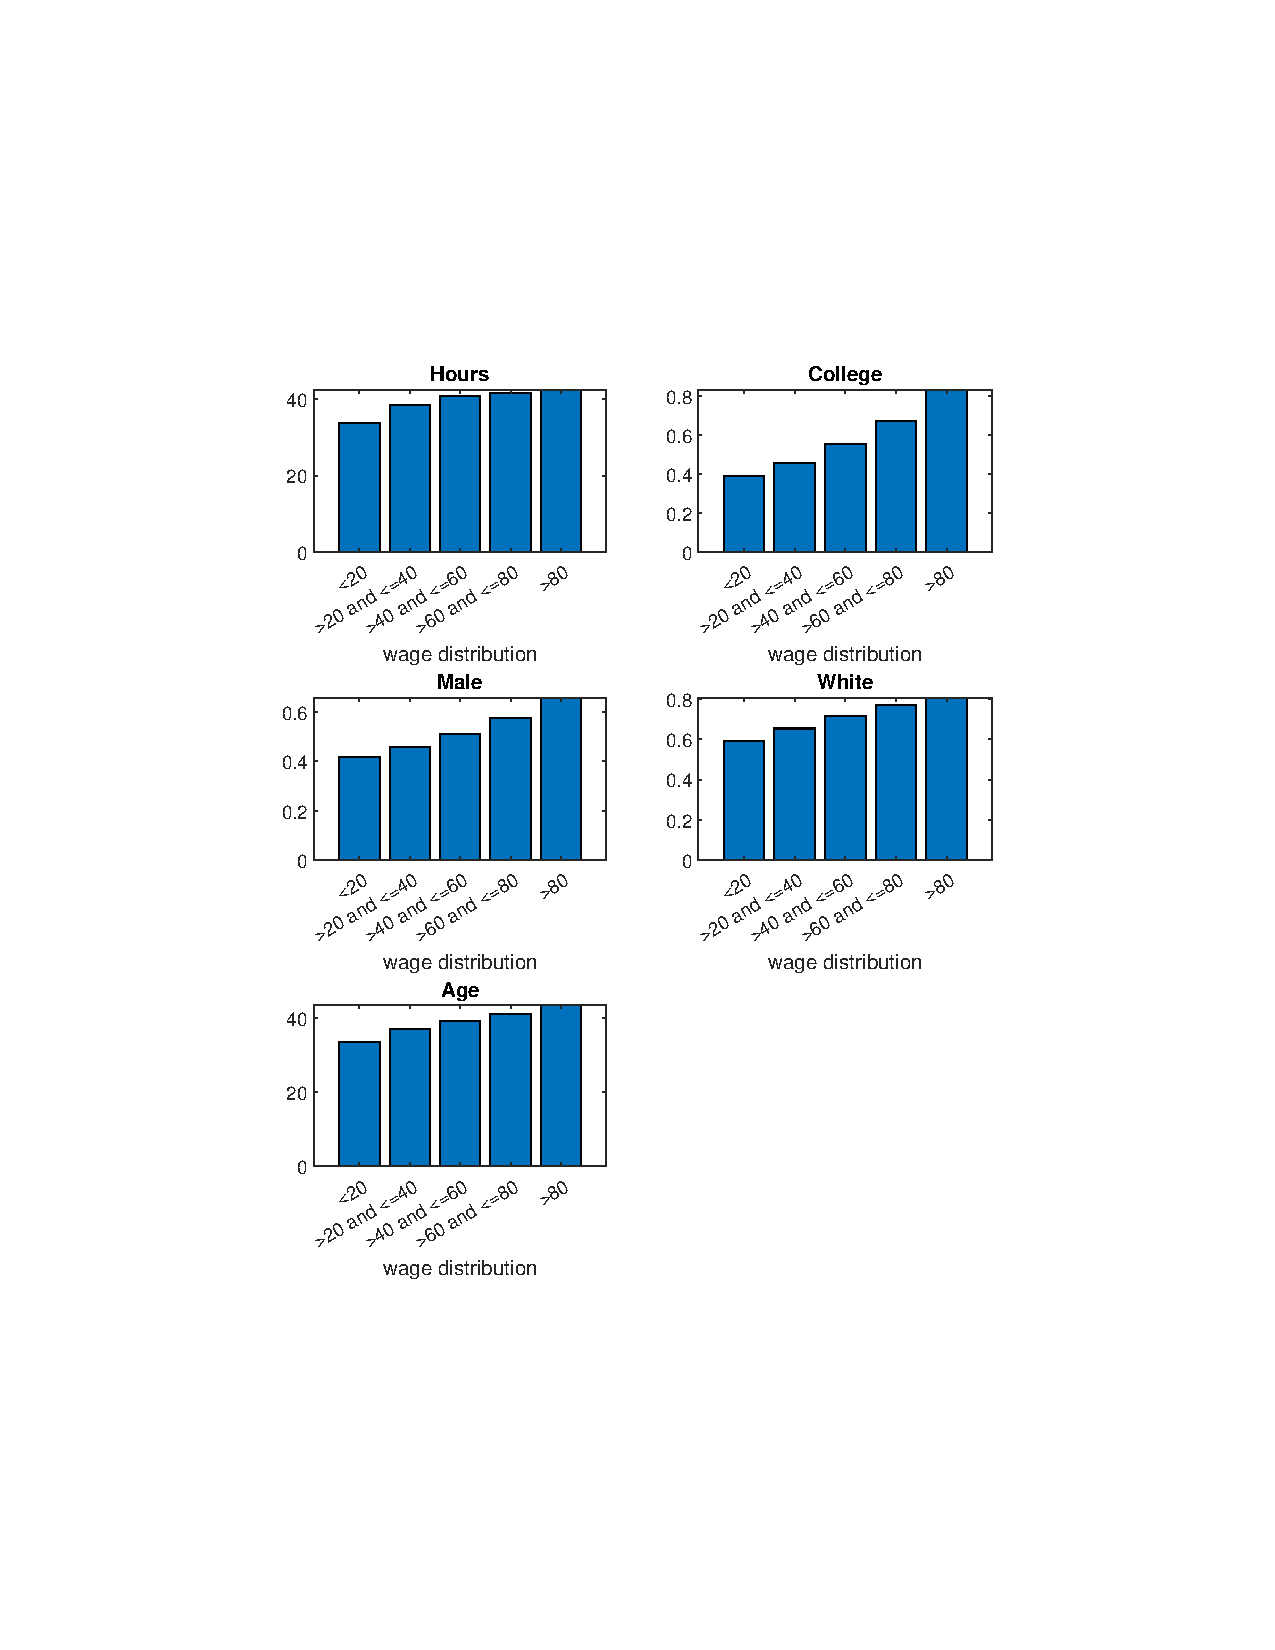
\includegraphics[width=0.9\textwidth]{figures_final/char.pdf}
\label{CPS:char_us}
\end{figure}


\begin{figure}[h!]
\centering
\caption{Proportion of individuals in different industries.}
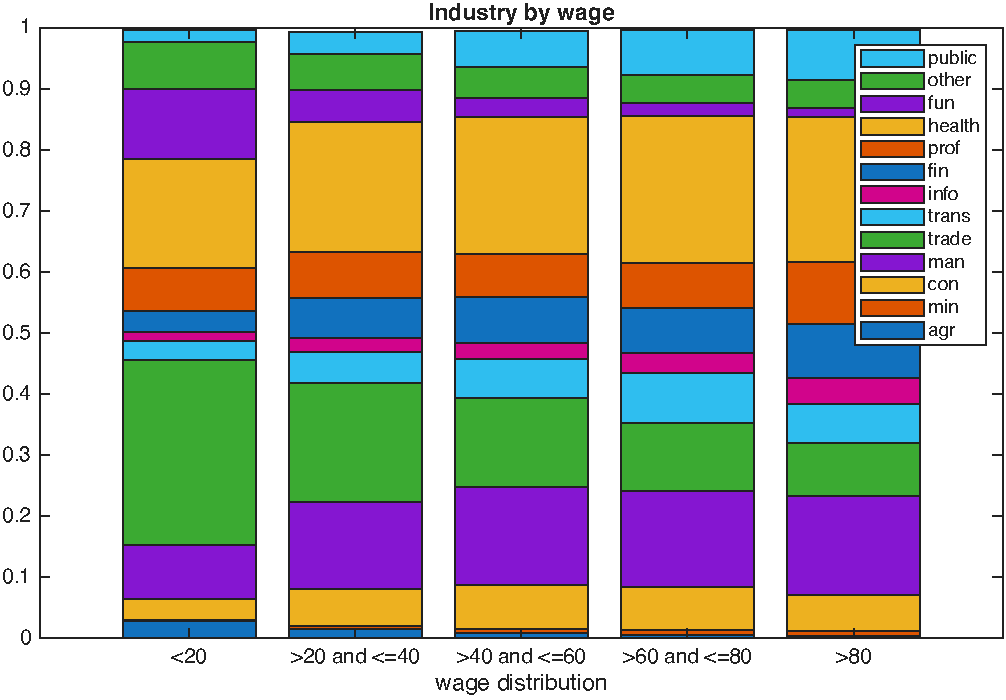
\includegraphics[width=0.9\textwidth]{figures_final/industry_by_wage_quintile_cepr_av_app.pdf}
\label{CPS:char_us1}

	{\footnotesize \textit{Notes:}  The proportions are averaged over the sample. agr is Agriculture, forestry, fishing and hunting. min is mining, con is construction, man is manufacturing, trade is wholesale and retail trade, trans is transport and utilities, info is information, fin is financial activities, prof is professional and business services, health is education and health services, fun is leisure and hospitality, other is other services and public denotes public administration.\par}

\end{figure}

Figure \ref{CPS:char_us} provides information regarding the characteristics of
the earnings distribution. Respondents in the right tail of the distribution
tend to be older, better educated, are likely to work longer hours and be white and Male. Figure \ref{CPS:char_us1} shows industry of employment across the wage distribution. At the left tail, industries such as wholesale and retail trade, health, leisure and manufacturing are important.
\newline As discussed above, we also employ the longitudinally matched version of CPS provided by the \href{https://cps.kansascityfed.org/}{Kansas Fed}. We employ the variable {wageperhrclean82} as our measure of hourly earnings. This series is deflated by CPI. The change in hours is constructed as the difference in the log of hours82 and {hours82\_tm12} where the former denotes a consistent series constructed using actual or usual hours and the latter is the 12 month lag of this variable. We construct the rate of transition from employment using the labour market status variable mlr76 and the 12 month lag of this variable {mlr76\_tm12}. As discussed in the text, we impute earnings for individuals that are not employed or do not report earnings data. To do this we regress earnings on experience and individual characteristics  including gender, occupation, industry of employment, geographical characteristics (US state, metropolitan indicator) and race. The fitted values from this regression are used to obtain imputed earnings.The coefficients of the regression are shocked and used to produce predicted values. These are assigned to individuals with missing earnings data using predicted mean matching. We produce 5 replicates, with the final imputed data taken to be the mean across these replications.   

\subsection{Comparison with aggregate data}\label{App:AggData}

The top panel of Figure \ref{Agg_h_us} compares aggregate actual hours from the
CPS to a measure of monthly hours from the Bureau of Labour statistics
(average weekly hours of production and non-supervisory employees). The CPS data captures the
main movements in the aggregate data fairly well.
%--------------------------------------------
\begin{figure}[h!]
\centering
\caption{Comparison of survey based total hours (blue) with aggregate (orange).}
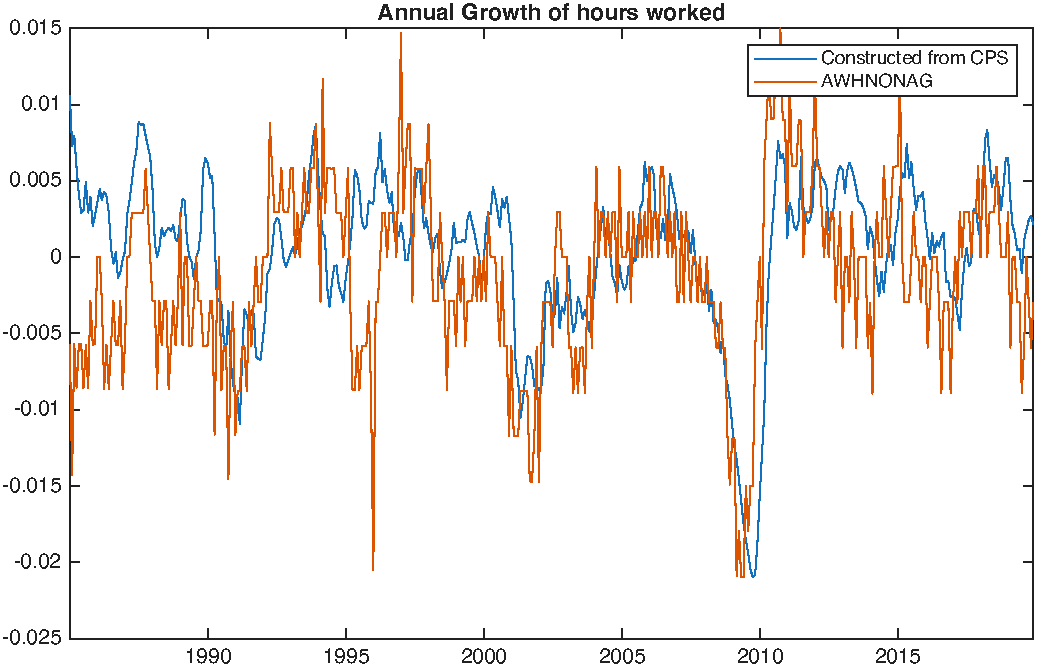
\includegraphics[width=0.9\textwidth]{figures_final/ag_hours.pdf}
\label{Agg_h_us}
\end{figure}
%-----------



\clearpage
\newpage


\section{Priors and estimation of the FAVAR}\label{App:PriorPosterior}
\setcounter{figure}{0}
\setcounter{table}{0}

The FAVAR model is defined by the following equations:%
\begin{equation}
X_{it}=c_{i}+b_{i}\tau +\Lambda_{i} F_{t}+\xi _{it}  \label{obs_app}
\end{equation}%
\begin{eqnarray}
Y_{t} &=&c+\sum\limits_{j=1}^{P}\beta _{j}Y_{t-j}+u_{t}  \label{trans_app} \\
cov\left( u_{t}\right)  &=&\Sigma =A_{0}A_{0}^{\prime }
\end{eqnarray}

Where $Y_{t}=\underset{N\times 1}{\underbrace{\left( 
\begin{array}{c}
R_{t} \\ 
F_{t}%
\end{array}%
\right) }}$, $R_{t}$ denotes the 1 year interest rate, $i=1,2,..,M$ denotes the cross-sectional dimension of the panel data-set $X_{it}$ while $t=1,2,..,T$ is the dimension.
As described in \citet{BLL:2020}, the factors can be consistently estimated using a principal components (PC) estimator. In particular, the factor
loadings are estimated via PC analysis of the first differenced data $
\Delta X_{it}$. With these in hand, the factors are estimated as $\hat{F}_{t}=\frac{1}{M}\left(\hat{\Lambda}^{\prime }\tilde{X_{t}}\right) $. Here,$\Lambda$ is the matrix of factor loadings, $\tilde{X_{t}}$ is given by $\left(x_{1t},x_{2t},...,x_{Mt}\right)$ where $x_{it}=X_{it}-\hat{c}_{i}-\hat{b}_{i}\tau $ Note that \citet{BLL:2020} describe a procedure to check if the $ith$ series contains a linear trend and that $\hat{b}_{i}$ is different from zero.

Given the estimated factors, the VAR in equations \ref{trans_app} is
estimated using a Bayesian methods.

\subsection{Priors}

Denote the var coefficients as $B=vec\left( \left[ \beta _{1},\beta
_{2},..,\beta _{P},c\right] \right) $.  
We follow \citet{banbura2007bayesian} and use a Natural Conjugate prior
implemented via dummy observations. The priors are implemented by the dummy observations $y_{D}$ and $x_{D}$ that are defined as:

\begin{equation}
y_{D}=\left[ 
\begin{array}{c}
\frac{diag\left( \gamma _{1}s_{1}...\gamma _{n}s_{n}\right) }{\kappa } \\ 
0_{N\times \left( P-1\right) \times N} \\ 
diag\left( s_{1}...s_{n}\right)  \\ 
.............. \\ 
0_{EX\times N}%
\end{array}%
\right] ,\ \ \ \ \ \ x_{D}=\left[ 
\begin{array}{c}
\frac{J_{P}\otimes diag\left( s_{1}...s_{n}\right) }{\kappa }\text{ }%
0_{NP\times EX} \\ 
..............\ \ \ \ \ \ \  \\ 
\text{ }0_{N\times (NP)+EX} \\ 
.............. \\ 
0_{EX\times NP}\text{ \ \ \ \ \ \ \ \ }I_{EX}\times 1/c%
\end{array}%
\right] 
\end{equation}%
where $J_{P}=diag(1,2,...,P)$, $\gamma _{1}$ to $\gamma _{n}$ denote the
prior mean for the parameters on the first lag obtained by estimating
individual AR(1) regressions, $s_{1}$ to $s_{n}$ is an estimate of the
variance of the endogenous variables obtained individual AR(1) regressions, $%
\kappa $ measures the tightness of the prior on the autoregressive VAR
coefficients, and $c$ is the tightness of the prior on the remaining
regressors. We set $\kappa =0.2$ and $c=1000$. We also implement priors on the
sum of coefficients (see \citet{banbura2007bayesian}). The dummy observations
for this prior are defined as:%
\begin{equation}
\tilde{y}_{D}=\frac{diag\left( \gamma _{1}\mu _{1}...\gamma _{n}\mu
_{n}\right) }{\tau },\tilde{x}_{D}=\left( 
\begin{array}{cc}
\left( 1_{1\times P}\right) \otimes \frac{diag\left( \gamma _{1}\mu
_{1}...\gamma _{n}\mu _{n}\right) }{\tau } & 0_{N\times EX}%
\end{array}%
\right) 
\end{equation}%
where $\mu _{i}$ is the sample average of the $ith$ variable. As in \citet{banbura2007bayesian} we set $\tau =10\kappa $. The total number of dummy observations is $T_{D}$.


\subsection{MCMC algorithm}

\citet{banbura2007bayesian} show that posterior distribution can be written
as:%
\begin{equation}
g\left( \Sigma |Y\right) \sim iW\left( \bar{\Sigma},T_{D}+2+T-K\right) 
\label{pos1}
\end{equation}

\begin{equation}
g\left( B|\Sigma ,Y\right) \sim N\left( \bar{B},\Sigma \otimes \left(
X_{\ast }^{\prime }X_{\ast }\right) ^{-1}\right)   \label{pos2}
\end{equation}%
where $iW$ denotes the inverse Wishart distribution, $K$ denotes the number of regressors in each
equation of the VAR model. Note that  $Y_{\ast }=\left( 
\begin{array}{c}
Y \\ 
y_{D} \\ 
\tilde{y}_{D}%
\end{array}%
\right) $ and $X_{\ast }=\left( 
\begin{array}{c}
X \\ 
x_{D} \\ 
\tilde{x}_{D}%
\end{array}%
\right) $, $X$ collects the regressors, and 
\begin{eqnarray*}
\tilde{B} &=&\left( X_{\ast }^{\prime }X_{\ast }\right) ^{-1}\left( X_{\ast
}^{\prime }Y_{\ast }\right)  \\
\bar{B} &=&vec\left( \tilde{B}\right)  \\
\bar{\Sigma} &=&\left( Y_{\ast }-X_{\ast }\tilde{B}\right) ^{\prime }\left(
Y_{\ast }-X_{\ast }\tilde{B}\right) 
\end{eqnarray*}%
Posterior draws can be easily generated by drawing $\Sigma $ from the
marginal distribution in \ref{pos1} and then $b$ from the conditional
distribution in equation \ref{pos2}. We set the number of draws to 21,000
with a burn-in of 1,000. We retain every second draw after the burn-in period. 

\section{IV Identification}\label{A:IV}

\label{App:IV} For a given draw of $B,\Sigma $ and $u_{t}$%
, we obtain the first column of $A_{0}$by using the
procedure proposed by \cite{MR:2013}. We
assume that the instrument is relevant and exogenous: %
\begin{eqnarray*}
cov\left( m_{t},\varepsilon _{1t}\right)  &=&\alpha  \\
cov\left( m_{t},\varepsilon _{t}^{-}\right)  &=&0
\end{eqnarray*}%
where $\varepsilon _{1t}$ denotes the structural shock of
interest that is ordered first for convenience, while $\varepsilon _{t}^{-}$%
 represent all remaining shocks and $\varepsilon _{t}=\left( 
\begin{array}{cc}
\varepsilon _{1t} & \varepsilon _{t}^{-}%
\end{array}%
\right) $. Re-writing the relevance and exogeneity conditions in
vector form: %
\begin{align}
E(m_{t}\varepsilon _{t}^{\prime })& =[\alpha \ \ 0]  \label{mr1} \\
E(m_{t}\varepsilon _{t}^{\prime }A_{0}^{\prime })& =[\alpha \ \
0]A_{0}^{\prime }  \label{mr2} \\
E(m_{t}u_{t}^{\prime })& =\alpha a_{0}  \label{mr3}
\end{align}%
where $a_{0}$ is a $(1\times R)$ vector
corresponding to the first row of $A_{0}^{\prime }$ (hence first
column of $A_{0}$). An estimate of $E(m_{t}u_{t}^{\prime })=\left( 
\begin{array}{c}
E(m_{t}u_{1t}^{\prime }) \\ 
E(m_{t}u_{2t}^{\prime }) \\ 
. \\ 
. \\ 
E(m_{t}u_{Nt}^{\prime })%
\end{array}%
\right) ^{\prime }$ can be easily obtained by using a linear
regression. However, $\alpha $ on the RHS of equation \ref{mr3} is
unknown. This parameter can be eliminated by normalising the left and the
right hand side by dividing by the first element of $E(m_{t}u_{t}^{\prime })
$ and $a_{0}$, respectively. Therefore the impulse vector
to a unit shock is given by $\tilde{a}_{0}=\left( 
\begin{array}{c}
1 \\ 
\frac{E(m_{t}u_{2t}^{\prime })}{E(m_{t}u_{1t}^{\prime })} \\ 
. \\ 
. \\ 
\frac{E(m_{t}u_{Nt}^{\prime })}{E(m_{t}u_{1t}^{\prime })}%
\end{array}%
\right) ^{\prime }$ . 

%\clearpage
%\newpage

\section{Robustness}\label{App:Rob}
\setcounter{figure}{0}
\setcounter{table}{0}

\subsection{Identification}

We employ the instrument of \cite{MAR:2020}. \cite{MAR:2020} argue that high frequency
instruments such as those used in \cite{GK:2015} contain information about
the policy shock and a signal regarding central bank's information about the
state of the economy. \cite{MAR:2020} construct their proxy as the high
frequency changes in federal funds futures that are orthogonal to Greenbook
forecasts and data revisions.

\begin{figure}[h!]
        \centering
                \caption{Response of hours worked}
   \includegraphics[width=0.9\textwidth]%
{figures_final/figure_mpi.pdf}%
                \label{fig:CPS_robustness1}
                
                	{\footnotesize \textit{Notes:} Identification using the instrument of \cite{MAR:2020}. The blue line and shaded area represent the response at a 6-month horizon, while the red line and shaded area illustrate the response at a 2-year horizon.\par}

    \end{figure}
    
  Figure \ref{fig:CPS_robustness1} shows the response of the distribution of hours to a contractionary policy shock obtained from this model. As in the benchmark case, hours increase towards the left tail of the earnings distribution.


\begin{figure}[h!]
        \centering
                \caption{Response of hours worked}                
              \includegraphics[width=0.9\textwidth]%
{figures_final/figure_sign.pdf}%
                \label{fig:CPS_robustness2}

                	{\footnotesize \textit{Notes:} Identification using sign restrictions: The blue line and shaded area represent the response at a 6-month horizon, while the red line and shaded area illustrate the response at a 2-year horizon.\par}
    \end{figure}
    
    As an alternative identification scheme, we employ sign restrictions. We assume that a contractionary monetary policy shock increases the one year rate,the Federal Funds rate, the unemployment rate and the excess bond premium and leads to a decrease in CPI and industrial production. The restrictions are imposed on the first 6 periods after the shock. Figure \ref{fig:CPS_robustness2} shows the response of hours to one standard deviation shock. While the response are less precisely estimated, the point to the conclusions obtained from the benchmark model. A contractionary monetary policy shock leads to an increase in hours at the left tail of the distribution.



\clearpage
\newpage

 \subsection{Hours by industry and by education attainments}\label{A:ind_edu}
  \begin{figure}[ht]
    \centering
    \caption{Proportion of individuals in different industries. }%
    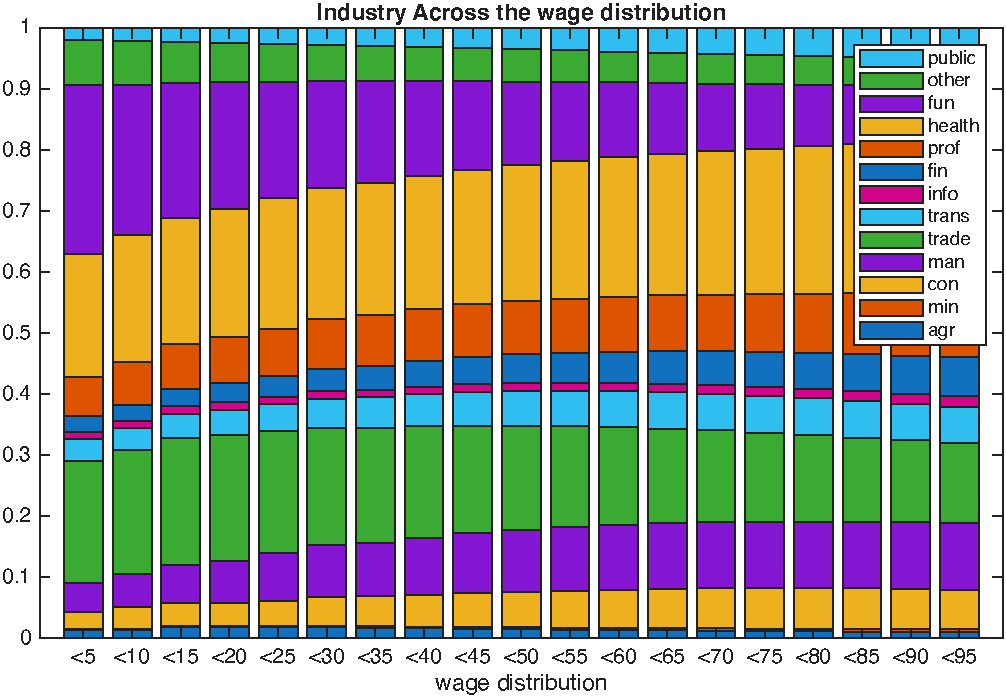
\includegraphics[width=6in,height=7in,scale = 0.5]{figures_final/industry_by_wage_quintile_cepr_av.pdf}
    \label{ind}%

                    	{\footnotesize \textit{Notes:} The proportions are averaged over the sample. agr is Agriculture, forestry, fishing and hunting. min is mining, con is construction, man is manufacturing, trade is Wholesale and retail trade, trans is transport and utilities, info is information, fin is financial activities, prof is professional and business services, health is education and health services, fun is leisure and hospitality, other is other services and public denotes public administration. \par}
   \end{figure}

Figure \ref{ind} shows the proportion of workers in 13 key industries across the  overall wage distribution. It is clear the left tail features workers in a variety of industries with the bulk employed in wholesale and retail trade, leisure and hospitality  and education and health services. Construction constitutes a relatively small proportion of the total.
 \begin{figure}[ht]
\caption{IRF of hours at the 6 mth horizon to a monetary contraction. }%
    \centering
     %\includegraphics[trim=left bottom right top, clip]
    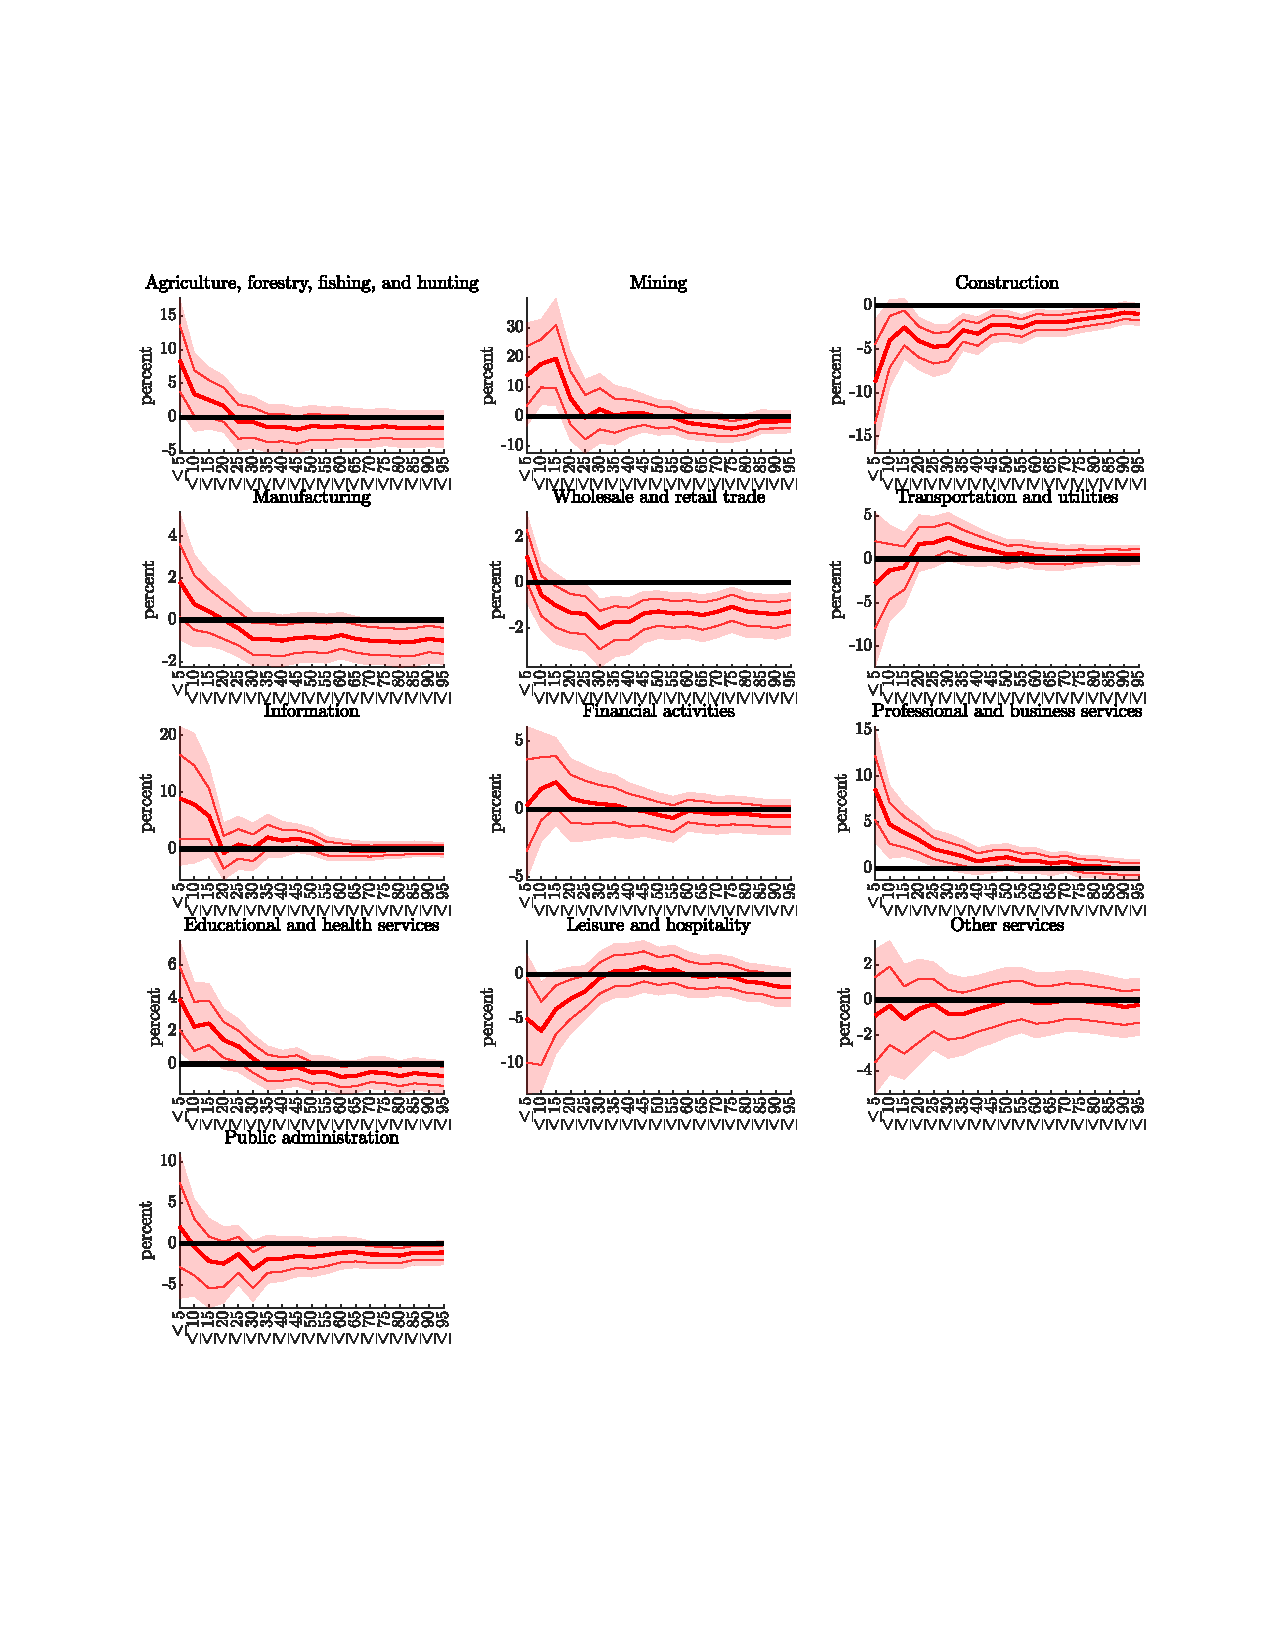
\includegraphics[width=\textwidth]{figures_final/hours_ind.pdf}
    
\label{irf_ind}%

{\footnotesize \textit{Notes:} The X-axis of each figure denotes the percentiles of the earnings distribution. \par}
   \end{figure}

   We re-estimate our benchmark model, splitting hours in each wage percentile group by the industry. In other words, for each group  defined by the wage distribution (i.e. less than the 5th percentile, less than 10th percentile and so on until the 95th percentile of wage), we split hours for individuals in to the 13 industry groups discussed above. \footnote{The model has a substantially larger cross-section and we include to 25 factors to account for the aggregate and disaggregated variables adequately. To keep the model computationally tractable, we reduce the number of lags to $6$.}
   Figure \ref{irf_ind} presents the impulse response of hours in each industry along the wage distribution. The responses at the left tail vary substantially. Sectors such as manufacturing, wholesale and retail trade and Education and health services show an increase in hours at the left tail after a monetary contraction. Some sectors such as construction, leisure and hospitality are more cyclical with hours declining at the left tail. 

   \begin{figure}[ht]
    \centering
\caption{Proportion of individuals with education less than high school (LTHS), high school (HS), some college (somecollege), college and advanced degrees (advanced).}%    
    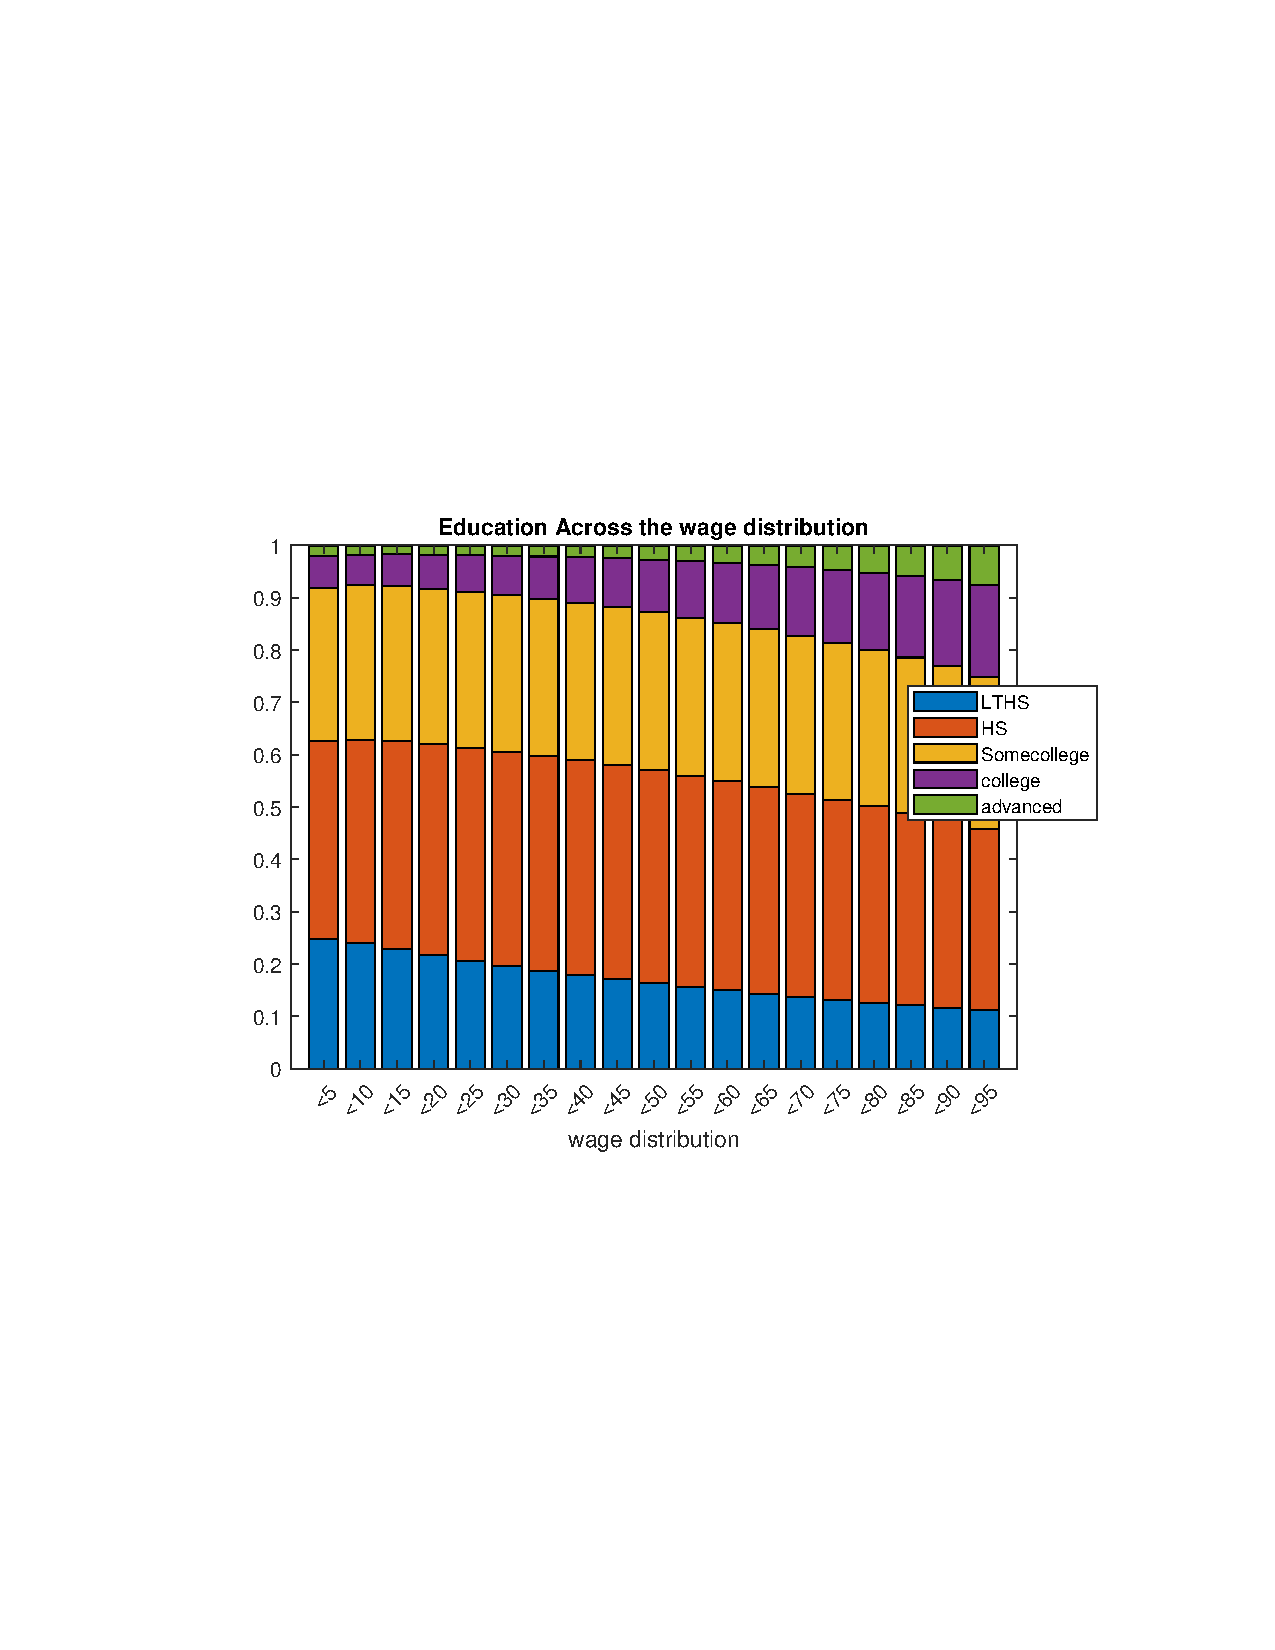
\includegraphics[width=\textwidth]{figures_final/college_by_wage2.pdf}
    

\label{college2}%
{\footnotesize \textit{Notes:} The proportions are averaged over the sample. \par}

   \end{figure}

Figure \ref{college2} shows that the left tail of the wage distribution is dominated by individuals with school education and some college.

  \begin{figure}[ht]
    \centering
\caption{Employees by level of education in each industry for individuals earning below the 20th percentile of wage. }%    
    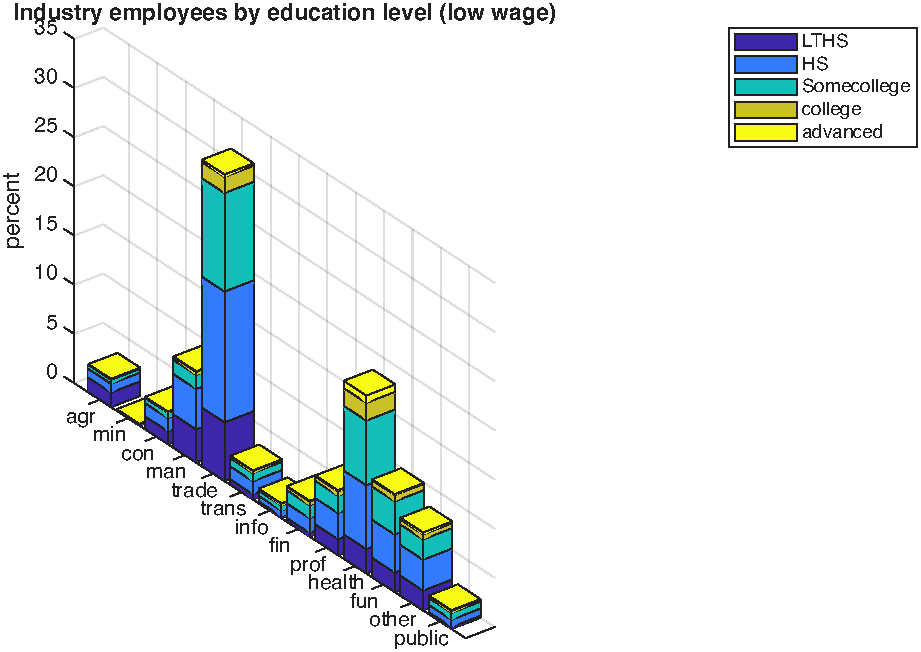
\includegraphics[width=\textwidth]{figures_final/college_by_wage3.pdf}
\label{college3}%

   {\footnotesize \textit{Notes:} Proportion of individuals with education less than high school (LTHS), high school (HS), some college (somecollege), college and advanced degrees (advanced). The proportions are averaged over the sample.  \par}

   \end{figure}

Figure \ref{college3} zooms in on employment by industry/education level for the left tail of the wage distribution. As noted above, Wholesale and Retail trade, Health and Education are important sectors of low wage employees. This figure shows that in these industries, most employees have high school education, followed by those with some college education.  


We re-estimate our benchmark model, splitting hours in each wage percentile group by the level of education. In other words, for each group  defined by the wage distribution (i.e. less than the 5th percentile, less than 10th percentile and so on until the 95th percentile of wage), we split hours for individuals with different level of education. We include average hours for each wage group in the FAVAR model.

 \begin{figure}[ht]
    \centering
\caption{IRF of hours at the 6mth horizon to a monetary contraction}%
%\includegraphics[trim=left bottom right top, clip]
    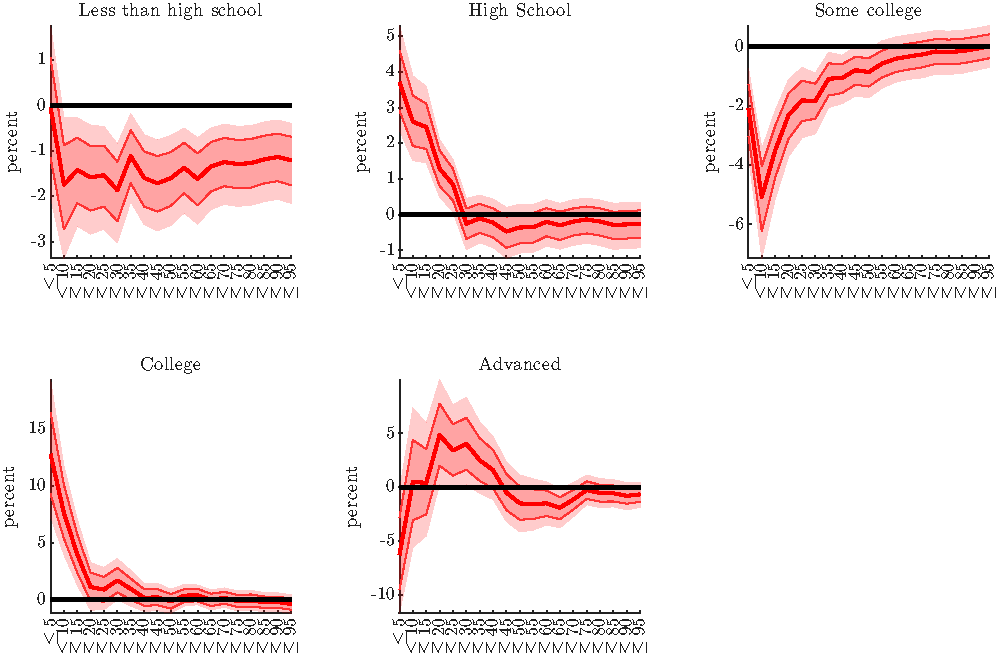
\includegraphics[width=\textwidth]{figures_final/hours_educ1.pdf}
    \label{irf_educ1}%
   \end{figure}

Figure \ref{irf_educ1} shows the response of hours in wage percentile for the different education groups. While the response of LTHS and somecollege displays strong cyclical behavior, hours of low wage individuals with high school or college education increases substantially.


\clearpage

\subsection{Response of real wages}   \label{A:realwages}

Figure \ref{FF:wages:IRF} reports the responses of real wages both in the aggregate and across different percentiles of the income distribution. We find that for individuals in the middle and upper parts of the distribution, real wages and hours worked both decline following a monetary tightening. This pattern is consistent with a reduction in labor demand.

In contrast, for individuals in the lower end of the distribution, real wages also decline, but hours worked increase. This divergence suggests that, in this group, an increase in labor supply is the dominant force driving the response. The overall picture thus points to heterogeneous labor market adjustment mechanisms across the income distribution, with labor supply playing a more prominent role for lower-income workers.


\begin{figure}[ht!]
	\caption{Responses of real wages after monetary policy tightening.}
%	\centering\includegraphics[width=\textwidth]{figures_final/test3}
	\centering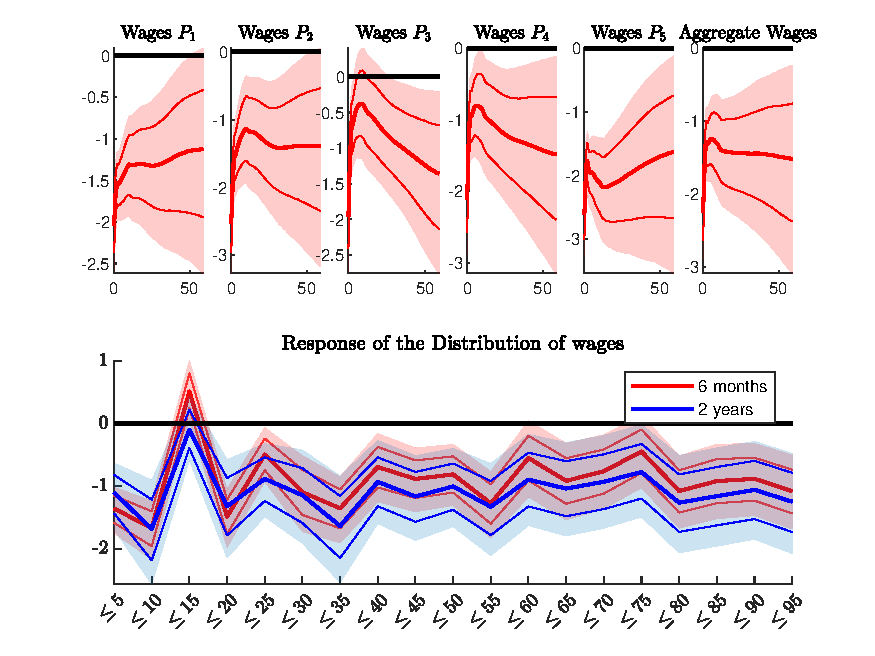
\includegraphics[width=\textwidth]{figures_final/figure_wages.pdf}
	\label{FF:wages:IRF}
	{\footnotesize \textit{Notes:} The top panels show the response of the real wages at different quintile of the wage distribution and the aggregate real wages (rightmost panel). The bottom panel displays the distribution of the responses of real wages six months (red) and two (blue) years after the shock. Shaded areas (solid lines) 68 (90)\% confidence sets. \par}
\end{figure}


%\clearpage
%\subsection{Response of hours for full-time workers}
%We restrict the sample to full-time workers in the CPS by setting the variable lfdetail76 equal to either $1$ or $2$. For this exercise we use the  \hyperlink{https://cps.kansascityfed.org/}{Kansas Fed} extract.
%    \begin{figure}[ht]
%    \centering
     %\includegraphics[trim=left bottom right top, clip]
%    \includegraphics[width=6in,height=7in,scale = 0.5, clip=true,trim = 2cm 4cm 2cm 4cm]{figures_final/figure_ft.pdf}   
%\caption{IRF of hours for full-time employees}%
%\label{fig:hours_full}
%   \end{figure}
%As shown in figure \ref{fig:hours_full}, hours increase at the left tail of the earnings distribution after a monetary contraction. 


\clearpage
\newpage

\section{Sample of Individuals Employed Continuously for Three Months}\label{A:SS}
 \begin{figure}[ht]
    \centering
    \caption{IRF of hours for Individuals Employed Continuously for Three Months}%
     %\includegraphics[trim=left bottom right top, clip]
    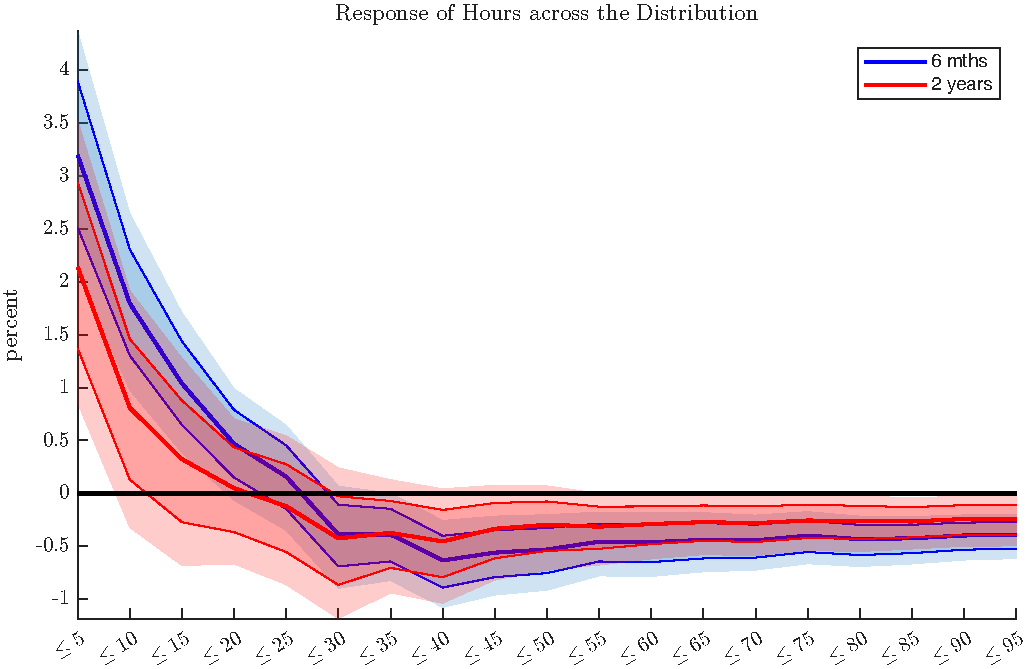
\includegraphics[width=\textwidth]{figures_final/figure_panel3M.pdf}
\label{fig:hours_3M}
   \end{figure}
We restrict the sample to workers employed for three months by setting the variables \texttt{mlr76}, \texttt{mlr76\_tm1}, and \texttt{mlr76\_tm2} equal to 1. For this exercise we use the  \href{https://cps.kansascityfed.org/}{Kansas Fed} extract. Figure \ref{fig:hours_3M} shows that Hours for this cohort go up at the left tail of the Wage distribution after a contractionary monetary policy shock.

\clearpage
\section{TANK model with Borrowers and Savers}\label{A:BSmodel}
A simple way to characterize the household heterogeneity and retain analytical tractability is to consider a two agents model where one type of agents are net \emph{borrower} (indexed with $B$) and the  other net \emph{saver} (indexed with $S$), as in \citet{BMP:2013}.\footnote{See their paper for details on the model derivation. Relative to them we simplify it further by abstracting from government debt, expenditure, and redistribution concerns. We follow \citet{Bilbiie:2019} and assume that there is a production subsidy that induces marginal cost pricing which implies that the steady state of marginal costs is 1 which simplifies substantially the steady state and the log-linearized conditions.} The key features of this class of models are that borrowers are more impatient than savers, have no access to government bonds, and can borrow up to a limit. Following \cite{Bilbiie:2019} and \cite{MNS:2016} we consider an economy where the monetary authority can effectively choose the real rate which makes the algebra simpler.

The key equations of the log-linearized model are reported in table \ref{tab:TANKBS_main}.%, where all variables are expressed in log deviation from steady state and $x_{t+1|t}$ represent the time $t$ conditional expectation of time $t+1$ variable. 
\begin{table}[h!]
\begin{center}
\begin{tabular}{ccc}
\hline
\hline
\multicolumn{3}{c}{Log-linearized Conditions}\\
\hline
1: & Labor Supply S & $\nu \hat{H}^S_{t} =\hat{w}_{t}-\sigma^{-1} \hat{c}^S_{t}$ \\
2: & Euler S &  $ \hat{c}_{t}^{S} =\hat{c}_{t+1|t}^{S}-\sigma\left(\hat{R}_{t}-\hat{\Pi}_{t+1|t}\right)$\\
3: & Labor Supply B & $\nu  \hat{H}^B_{t} = \hat{w}_{t}-\sigma^{-1}  \hat{c}^B_{t}$ \\
4: & Budget constraint B & $\hat{c}^B_{t}\, \gamma+{\bar{D}}(\hat{R}_{t-1}-\hat{\Pi}_{t})= \left({\hat{w}}_{t}+\hat{H}^B_{t}\right)$\\
5: & Phillips Curve & $ \hat{\Pi}_{t} =\beta E_{t}  \hat{\Pi}_{t+1}+ \kappa  \hat{w}_{t}$\\
6: & Aggregate C & $ \hat{c}_t=\lambda \gamma  \hat{c}^B_t+(1-\lambda \gamma) \hat{c}^S_t$\\
7: & Aggregate B & $ \hat{c}_t=\hat{H}_t=\lambda  \hat{H}^B_t+(1-\lambda) \hat{H}^S_t$\\
8: & Taylor Rule & $  \hat{R}_{t} = \hat{\Pi}_{t+1|t}+\epsilon^m_{t} $\\
\hline
\hline
\end{tabular}
\end{center}
\caption{Log-linearized Conditions of Savers/Borrowers model}\label{tab:TANKBS_main}
\end{table}

This section follows a different notational convention that the one used for the HANK model in the main text. Small case letters represent real variables while capital letters represent nominal variables or hours worked. A 'hat' on top of the variable denotes percentage deviations from the steady state. 
The assumption that borrowers discount more future consumption, $\beta^B<\beta^S=\beta$, implies that they become net borrower in equilibrium with the borrowing limit ($\bar{D}$) always binding.\footnote{Note that in equation (4) in table \ref{tab:TANKBS_main} $\bar{D}$ is effectively divided by the steady state of total income/consumption. But this is =1 one in this simple set up. }  $\gamma$ is a steady state parameter which captures the consumption inequality between borrowers and savers, i.e. $\gamma=c^B/c=1+\bar{D}(\beta-1)<1$. Notice that when $\bar{D}=0 \rightarrow \gamma=1$ and the model is identical to the one with Savers and HTM consumers.\footnote{In that set up, \cite{Bilbiie:2008} showed that $\sigma<1$ is the condition for the hours of hand-to-mouth agents to increase following a decline in their income.} In this model,  a fraction of agents are not on the Euler equation and cannot optimize intertemporally. Importantly, and differently from a model with HTM that are not net borrowers, a change in the nominal rate will have an impact not only on the time $t$ consumption and labor supply decision but also on the $t+1$ decisions because the debt repayments at $t+1$ depend on the time $t$ interest rates. 
%\todo[inline]{Check stability of this model and the condition under which the IS curve slope changes sign.}

Under mild conditions, borrowers have an incentive to increase their labor supply after an interest rate hike; this is formalized in the following proposition.
\begin{proposition}\label{T:propBS}
Under SADL ($\lambda<\frac{1}{1+\nu(1+\bar{D}\kappa)}$) and $\sigma<\frac{1+\bar{D}\kappa}{\gamma}$, a rate hike at time $t$ induces an increases in the borrowers labor supply both at time $t$ and $t+1$.
\end{proposition}

The proof is on the next page. At the core of this result, we have that consumption and the labor supply of the borrowers move in opposite directions. This can be appreciated when combining the time $t+1$ optimal response of borrowers in terms of consumption and labor supply after a monetary policy shock which are\footnote{The time $t$ optimal responses are analogous but more involved. To ease the notation we only discuss the time $t+1$ decisions.}
\begin{align*} 
\hat{H}^B_{t+1} &= \frac{\bar{D}(\nu \lambda \gamma \sigma- 1 +\lambda)}{ (\nu \lambda -1+\lambda) (1+\gamma\nu\sigma)}\epsilon^m_{t},\\
\hat{c}^B_{t+1} &= \frac{\nu\sigma\bar{D}}{ (\nu \lambda -1+\lambda) (1+\gamma\nu\sigma)}\epsilon^m_{t}.  
\end{align*}
Combining the latter two equations we have that 
$$ \hat{c}^B_{t+1} = \frac{\nu\sigma}{\nu \lambda \gamma \sigma- 1 +\lambda}\hat{H}^B_{t+1}. $$
The numerator is positive. Notice that if the conditions of Proposition \ref{T:propBS} hold, we have $ \lambda < \frac{1}{1+\nu(1+\bar{D}\kappa)}< \frac{1}{1+\nu\sigma\gamma}$, which implies that $(1-\lambda-\nu \sigma\lambda \gamma)>0$; hence the denominator is negative.  %As mentioned this model nests the HtM model when $\bar{D}=0$. This holds true also for the sufficient conditions of Proposition \ref{T:propBS}; notice that when $\bar{D}=0 \rightarrow \gamma =1 \rightarrow \sigma <1$ and $\lambda < \frac{1}{1+\nu}$. 

\paragraph{Derivation of Proposition \ref{T:propBS}}\label{App:propBS}

% The derivation of Proposition \ref{T:propBS} is relativelly long since $\hat{R}_t$ enters the budget constrain of the Borrowers at $t+1$. This requires a backward induction solution approach, i.e. we first solve $t+1$, then given $t+1$ we solve for $t$. For convenience we report below the time $t+1$ equilibrium conditions. 

% \begin{table}[h!]
% \begin{center}
% \begin{tabular}{ccc}
% \hline
% \hline
% \multicolumn{3}{c}{Log-linearized Conditions}\\
% \hline
% 1: & Labor Supply S & $\nu \hat{H}^S_{t+1} =\hat{w}_{t+1}-\sigma^{-1} \hat{c}^S_{t+1}$ \\
% 2: & Euler S &  $ \hat{c}_{t+1}^{S} =\hat{c}_{t+2|t+1}^{S}-\sigma\left(\hat{R}_{t+1}-\hat{\Pi}_{t+2|t+1}\right)$\\
% 3: & Labor Supply B & $\nu  \hat{H}^B_{t+1} = \hat{w}_{t+1}-\sigma^{-1}  \hat{c}^B_{t+1}$ \\
% 4: & Budget constraint B & $\hat{c}^B_{t+1}\, \gamma+{\bar{D}}(\hat{R}_{t}-\hat{\Pi}_{t+1})= \left({\hat{w}}_{t+1}+\hat{H}^B_{t+1}\right)$\\
% 5: & Phillips Curve & $ \hat{\Pi}_{t+1} =\beta \hat{\Pi}_{t+2|t+1}+ \kappa  \hat{w}_{t+1}$\\
% 6: & Aggregate C & $ \hat{c}_{t+1}=\lambda \gamma  \hat{c}^B_{t+1}+(1-\lambda \gamma) \hat{c}^S_{t+1}$\\
% 7: & Aggregate B & $ \hat{c}_{t+1}=\lambda  \hat{H}^B_{t+1}+(1-\lambda) \hat{H}^S_{t+1}$\\
% 8: & Taylor Rule & $  \hat{R}_{t+1} = \hat{\Pi}_{t+2|t+1}+\epsilon^m_{t+1} $\\
% \hline
% \hline
% \end{tabular}
% \end{center}
% \caption{Log-linearized Conditions of Savers/Borrowers model}\label{tab:TANKBS}
% \end{table}

Recall that $\epsilon^m_{t+j} = 0$ for $j>0$ and $\epsilon^m_{t}\neq 0$.  This implies that from $t+2$ onward the economy is back to steady states and all quantities are zero. This means also that $ \hat{R}_{t+j} = \hat{\Pi}_{t+j+1|t+j}$ for $j>0$, which implies that 
$$ \hat{c}_{t+1}^{S} =0$$
The saver labor supply becomes
$$ \nu \hat{H}^S_{t+1} =\hat{w}_{t+1}$$
Using the borrowers BC we have 
\begin{align*}
\hat{c}^B_{t+1} \gamma+{\bar{D}}(\hat{R}_{t}-\hat{\Pi}_{t+1}) &= \left({\hat{w}}_{t+1}+\hat{H}^B_{t+1}\right)\\
\hat{c}^B_{t+1} \gamma+{\bar{D}}(\hat{\Pi}_{t+1|t}+\epsilon^m_{t}-\hat{\Pi}_{t+1}) &= (1+\nu)\hat{H}^B_{t+1} + 1/\sigma\hat{c}^B_{t+1} \\
1/ \sigma \hat{c}^B_{t+1}&= \frac{1+\nu}{\gamma\sigma-1} \hat{H}^B_{t+1} - \frac{\bar{D}}{\gamma\sigma-1} \epsilon^m_{t}
\end{align*}
notice that in absence of shocks in $t+1$ $\hat{\Pi}_{t+1} =\hat{\Pi}_{t+1|t}$. Combining the to labor supply conditions we have 
\begin{align*}
\nu \hat{H}^S_{t+1} + \sigma^{-1} \hat{c}^S_{t+1} &= \nu \hat{H}^B_{t+1} + \sigma^{-1} \hat{c}^B_{t+1}\\
\nu \hat{H}^S_{t+1}  &= \nu \hat{H}^B_{t+1} + \frac{1+\nu}{\gamma\sigma-1} \hat{H}^B_{t+1} - \frac{\bar{D}}{\gamma\sigma-1} \epsilon^m_{t}\\
\nu \hat{H}^S_{t+1}  &= \frac{1+\gamma\nu\sigma}{\gamma\sigma-1} \hat{H}^B_{t+1} - \frac{\bar{D}}{\gamma\sigma-1} \epsilon^m_{t}\\
\end{align*}
Combining the aggregate conditions we have
\begin{align*}
\lambda \gamma  \hat{c}^B_{t+1}+(1-\lambda \gamma) \hat{c}^S_{t+1} =&\lambda  \hat{H}^B_{t+1}+(1-\lambda) \hat{H}^S_{t+1}\\
\lambda \gamma \sigma\left[\frac{1+\nu}{\gamma\sigma-1} \hat{H}^B_{t+1} - \frac{\bar{D}}{\gamma\sigma-1} \epsilon^m_{t}  \right] =&\lambda  \hat{H}^B_{t+1}+(1-\lambda) \left[ \frac{1+\gamma\nu\sigma}{\nu(\gamma\sigma-1)} \hat{H}^B_{t+1} - \frac{\bar{D}}{\nu(\gamma\sigma-1)} \epsilon^m_{t}\right]\\
\hat{H}^B_{t+1}\left[\frac{(1+\nu)\lambda \gamma \sigma}{\gamma\sigma-1}  - \lambda  - (1-\lambda) \frac{1+\gamma\nu\sigma}{\nu(\gamma\sigma-1)}  \right] =& \left[\frac{\bar{D}\lambda \gamma \sigma}{\gamma\sigma-1} -  (1-\lambda) \frac{\bar{D}}{\nu(\gamma\sigma-1)} \right]\epsilon^m_{t}\\
\hat{H}^B_{t+1}\left[\frac{(1+\nu)\nu \lambda \gamma \sigma  - \lambda\nu(\gamma\sigma-1) - (1-\lambda) (1+\gamma\nu\sigma)}{\nu(\gamma\sigma-1)}   \right] =& \frac{\nu \lambda \gamma \sigma-(1-\lambda)}{ \nu(\gamma\sigma-1)} \bar{D}\epsilon^m_{t}\\
\hat{H}^B_{t+1}\left[\frac{\nu \lambda ( \gamma \sigma+\nu \gamma \sigma  - \gamma\sigma+1) - (1-\lambda) (1+\gamma\nu\sigma)}{\nu(\gamma\sigma-1)}   \right] =& \frac{\nu \lambda \gamma \sigma-(1-\lambda)}{ \nu(\gamma\sigma-1)} \bar{D}\epsilon^m_{t}\\
\hat{H}^B_{t+1} \frac{ (\nu \lambda -1+\lambda) (1+\gamma\nu\sigma)}{\nu(\gamma\sigma-1)} =& \frac{\nu \lambda \gamma \sigma-(1-\lambda)}{ \nu(\gamma\sigma-1)} \bar{D}\epsilon^m_{t}
\end{align*}
which yield to
\begin{align}
\hat{H}^B_{t+1} = \frac{\nu \lambda \gamma \sigma- 1 +\lambda}{ (\nu \lambda -1+\lambda) (1+\gamma\nu\sigma)} \bar{D}\ \epsilon^m_{t} \label{cvd:t2}
\end{align}
This implies that borrower consumption at time $t+1$ is
\begin{align*}
\hat{c}^B_{t+1} =&  \frac{\sigma(1+\nu)}{\gamma\sigma-1} \hat{H}^B_{t+1} - \frac{\sigma\bar{D}}{\gamma\sigma-1} \epsilon^m_{t}\\
=& \frac{\sigma(1+\nu)}{\gamma\sigma-1}  \frac{\nu \lambda \gamma \sigma- 1 +\lambda}{ (\nu \lambda -1+\lambda) (1+\gamma\nu\sigma)} \bar{D}\ \epsilon^m_{t} - \frac{\sigma\bar{D}}{\gamma\sigma-1} \epsilon^m_{t}\\
=& \epsilon^m_{t} \frac{\sigma\bar{D}}{\gamma\sigma-1}  \left[ \frac{(1+\nu)(- 1 +\lambda(1+\nu \gamma \sigma) ) - (\nu \lambda -1+\lambda) (1+\gamma\nu\sigma)}{ (\nu \lambda -1+\lambda) (1+\gamma\nu\sigma)} \right]\\
=& \epsilon^m_{t} \frac{\sigma\bar{D}}{\gamma\sigma-1}  \left[ \frac{-(1+\nu) + (1+\nu)\lambda(1+\nu \gamma \sigma) - \nu \lambda(1+\gamma\nu\sigma) +(1-\lambda) (1+\gamma\nu\sigma)}{ (\nu \lambda -1+\lambda) (1+\gamma\nu\sigma)} \right]\\
=& \epsilon^m_{t} \frac{\sigma\bar{D}}{\gamma\sigma-1}  \left[ \frac{-1-\nu+ 1+\gamma\nu\sigma}{ (\nu \lambda -1+\lambda) (1+\gamma\nu\sigma)} \right]\\
=& \epsilon^m_{t} \frac{\nu\sigma\bar{D}}{ (\nu \lambda -1+\lambda) (1+\gamma\nu\sigma)} 
\end{align*}
and wages 
\begin{align*}
{\hat{w}}_{t+1} &= \nu \hat{H}^B_{t+1}+1/\sigma \hat{c}^B_{t+1} \\
=&  \nu \frac{\nu \lambda \gamma \sigma- 1 +\lambda}{ (\nu \lambda -1+\lambda) (1+\gamma\nu\sigma)} \bar{D}\ \epsilon^m_{t} + \epsilon^m_{t} \frac{\nu\bar{D}}{ (\nu \lambda -1+\lambda) (1+\gamma\nu\sigma)} \\
=& \epsilon^m_{t} \bar{D} \nu \frac{\nu \lambda \gamma \sigma- 1 +\lambda + 1}{ (\nu \lambda -1+\lambda) (1+\gamma\nu\sigma)} \\
&=\epsilon^m_{t}  \frac{\bar{D} \nu \lambda}{\nu \lambda -1+\lambda} 
\end{align*}
and inflation 
\begin{align*}
\hat{\Pi}_{t+1} =\beta \hat{\Pi}_{t+2|t+1}+ \kappa  \hat{w}_{t+1} = \epsilon^m_{t}  \frac{\bar{D} \nu \lambda \kappa}{\nu \lambda -1+\lambda}
\end{align*}
Now, we are in a position to solve for time $t$. Solving the Euler equation forward we have  
$$ \hat{c}_{t}^{S} = - \sigma \epsilon^m_{t}$$
From the NKP we have an expression for today inflation
$$ \hat{\Pi}_{t} = \beta  {\hat{\Pi}}_{t+1|t} + \kappa {\hat{w}}_{t}  = \epsilon^m_{t}  \frac{\bar{D} \nu \lambda \kappa \beta}{\nu \lambda -1+\lambda} +  \kappa {\hat{w}}_{t}   $$
Using the borrowers BC we have 
\begin{align*}
\gamma\hat{c}^B_{t}+{\bar{D}}(\hat{R}_{t-1}-\hat{\Pi}_{t}) &= {\hat{w}}_{t}+\hat{H}^B_{t}\\
\gamma\hat{c}^B_{t}- \epsilon^m_{t} {\bar{D}} \frac{\bar{D} \nu \lambda \kappa \beta}{\nu \lambda -1+\lambda} -  {\bar{D}}\kappa \nu \hat{H}^B_{t} - {\bar{D}}\kappa /\sigma \hat{c}^B_{t}   &=    \nu \hat{H}^B_{t} + 1 /\sigma \hat{c}^B_{t}+\hat{H}^B_{t}
\end{align*}
which yields to 
\begin{align*}
 \hat{c}^B_{t}  &=\frac{\sigma(1+\nu(1+{\bar{D}}\kappa))}{\gamma\sigma-1-{\bar{D}}\kappa}\hat{H}^B_{t} + 
 \frac{\bar{D}^2 \sigma\nu \lambda \kappa \beta}{e_1e_0}\epsilon^m_{t}
\end{align*}
where $e_1=\gamma\sigma-1-{\bar{D}}\kappa$ and $e_0 = \nu \lambda -1+\lambda$.
Combining the labor supply decision we have 
\begin{align*}
\nu \hat{H}^S_{t} + \sigma^{-1} \hat{c}^S_{t} &= \nu \hat{H}^B_{t} + \sigma^{-1} \hat{c}^B_{t}\\
\nu \hat{H}^S_{t} - \epsilon^m_{t} &= \nu \hat{H}^B_{t} + \frac{1+\nu+\nu{\bar{D}}\kappa}{\gamma\sigma-1-{\bar{D}}\kappa}\hat{H}^B_{t} + 
 \frac{\bar{D}^2 \nu \lambda \kappa \beta}{(\gamma\sigma-1-{\bar{D}}\kappa)(\nu \lambda -1+\lambda)}\epsilon^m_{t}
\end{align*}
which yields to 
\begin{align*}
\hat{H}^S_{t}  &= \frac{1+\nu\gamma\sigma}{\nu(\gamma\sigma-1-{\bar{D}}\kappa)}\hat{H}^B_{t} + 
 \frac{\bar{D}^2 \nu \lambda \kappa \beta+ e_0e_1}{\nu e_0e_1}\epsilon^m_{t}
\end{align*}
where $e_1=\gamma\sigma-1-{\bar{D}}\kappa$ and $e_0 = \nu \lambda -1+\lambda$.

Combining the aggregate conditions at time $t$ we have 
\begin{align*}
  &\lambda \gamma  \hat{c}^B_{t}+(1-\lambda \gamma) \hat{c}^S_{t}=\lambda  \hat{H}^B_{t}+(1-\lambda) \hat{H}^S_{t}
\end{align*}
\begin{align*}
\lambda \gamma  &\left[ \frac{\sigma(1+\nu(1+{\bar{D}}\kappa))}{\gamma\sigma-1-{\bar{D}}\kappa}\hat{H}^B_{t} + 
 \frac{\bar{D}^2 \sigma\nu \lambda \kappa \beta}{e_1e_0}\epsilon^m_{t} \right]+(1-\lambda \gamma) [-\sigma\epsilon^m_{t}]\\
 &=\lambda  \hat{H}^B_{t}+(1-\lambda) \left[ \frac{1+\nu\gamma\sigma}{\nu(\gamma\sigma-1-{\bar{D}}\kappa)}\hat{H}^B_{t} +  \frac{\bar{D}^2 \nu \lambda \kappa \beta+ e_0e_1}{\nu e_0e_1}\epsilon^m_{t} \right]
\end{align*}
\begin{align*}
\hat{H}^B_{t}  &\left[ \frac{\lambda \gamma \nu\sigma(1+\nu(1+{\bar{D}}\kappa))}{\nu(\gamma\sigma-1-{\bar{D}}\kappa)} -\frac{\lambda\nu(\gamma\sigma-1-{\bar{D}}\kappa)}{\nu(\gamma\sigma-1-{\bar{D}}\kappa)} -  \frac{(1-\lambda)(1+\nu\gamma\sigma)}{\nu(\gamma\sigma-1-{\bar{D}}\kappa)} \right]\\
 &=\epsilon^m_{t} \left[\sigma(1-\lambda \gamma) -  \gamma\lambda\frac{\bar{D}^2 \sigma\nu \lambda \kappa \beta}{e_1e_0} + (1-\lambda)  \frac{\bar{D}^2 \nu \lambda \kappa \beta+ e_0e_1}{\nu e_0e_1} \right]
\end{align*}
Focusing on terms inside the left hand side square bracket we have
\begin{align*}
&\nu^{-1}e_1^{-1}\left[ \nu\lambda(\sigma\gamma + \sigma\gamma\nu(1+{\bar{D}}\kappa)) - \lambda\nu(\gamma\sigma-1-{\bar{D}}\kappa) - (1-\lambda)(1+\nu\gamma\sigma)  \right] \\
&= \nu^{-1}e_1^{-1}\left[	\nu\lambda(1 + \sigma\gamma\nu)(1+{\bar{D}}\kappa) - (1-\lambda)(1+\nu\gamma\sigma) 	\right] \\
&= \nu^{-1}e_1^{-1}(1 + \sigma\gamma\nu)(\nu\lambda(1+{\bar{D}}\kappa) -1+\lambda) 
\end{align*}
Focusing on terms inside the right hand side square bracket we have
\begin{align*}
&(\nu e_0e_1)^{-1}\left[\nu \sigma(1-\lambda \gamma) e_0e_1 -  \nu \gamma\lambda(\bar{D}^2 \sigma\nu \lambda \kappa \beta) + (1-\lambda) (\bar{D}^2 \nu \lambda \kappa \beta+ e_0e_1) \right]\\
&=(\nu e_0e_1)^{-1}\left[\nu \sigma(1-\lambda \gamma) e_0e_1 -  \nu \gamma\lambda(\bar{D}^2 \sigma\nu \lambda \kappa \beta) + (1-\lambda) \bar{D}^2 \nu \lambda \kappa \beta + (1-\lambda)e_0e_1 \right]\\
&=(\nu e_0e_1)^{-1}\left[e_0e_1(\nu \sigma(1-\lambda \gamma)+ 1-\lambda)  -  \nu \gamma\lambda\sigma\bar{D}^2\nu \lambda \kappa \beta + (1-\lambda) \bar{D}^2 \nu \lambda \kappa \beta \right]\\
&=(\nu e_0e_1)^{-1}\left[\nu \sigma e_0e_1+ e_0e_1(1-\lambda-\nu \sigma\lambda \gamma) + \bar{D}^2 \nu \lambda \kappa \beta(1-\lambda-\nu \sigma\lambda \gamma)  \right]\\
&=(\nu e_0e_1)^{-1}\left[\nu \sigma e_0e_1+ (e_0e_1 + \bar{D}^2 \nu \lambda \kappa \beta)(1-\lambda-\nu \sigma\lambda \gamma)  \right]\\
\end{align*}
Rearranging terms we have 
\begin{align}
\hat{H}^B_{t}  = \frac{\nu \sigma e_0e_1+ (e_0e_1 + \bar{D}^2 \nu \lambda \kappa \beta)(1-\lambda-\nu \sigma\lambda \gamma)}{(1 + \sigma\gamma\nu)(\nu\lambda(1+{\bar{D}}\kappa) -1+\lambda)( \nu \lambda -1+\lambda)} \ \epsilon^m_{t} \label{cvd:t1}
\end{align}
where $e_1=\gamma\sigma-1-{\bar{D}}\kappa$ and $e_0 = \nu \lambda -1+\lambda$. While still not very tractable we can derive a set of sufficient conditions such that the latter expression becomes positive. These conditions are 
\begin{enumerate}
\item $\lambda < \frac{1}{1+\nu(1+\bar{D}\kappa)}$% \rightarrow [\nu\lambda  (1+\bar{D}\kappa)  - 1 + \lambda]<0$
\item $\sigma < \frac{1+\bar{D}\kappa}{\gamma}$%\rightarrow (\sigma\gamma-1-\bar{D}\kappa)<0$
 \end{enumerate}
Condition 1 implies that $e_1=[\nu\lambda  (1+\bar{D}\kappa)  - 1 + \lambda]<0$; this implies also that $(\nu\lambda - 1 + \lambda)<0$. Thus, if condition 1 holds, the denominator is positive.
Condition 2 implies that $e_0 = (\sigma\gamma-1-\bar{D}\kappa)<0$; this implies also that $e_0e_1>0$. Moreover, if condition 2 hold, it is the case that 
$$ \lambda < \frac{1}{1+\nu(1+\bar{D}\kappa)}< \frac{1}{1+\nu\sigma\gamma}$$
The latter implies that $(1-\lambda-\nu \sigma\lambda \gamma)>0$. Therefore also the numerator is positive. These conditions imply also that the coefficient in \eqref{cvd:t2} is positive.

\clearpage

\section{One Asset HANK Appendix}\label{A:HANK}

\subsection{Steady State}\label{A:HANK_SS}


Table \ref{tab:income_states} summarizes the mapping between the discrete income states in the model and their corresponding positions in the income distribution. It shows that, in line with the data, both median consumption and labor supply increase monotonically with income. %While consumption rises proportionally more with income, hours worked exhibit a more gradual upward trend, reflecting the relatively flat labor supply elasticity across income groups at steady state.  
Figure \ref{fig:LS_PC} plots the labor supply policy as a function of assets for each income group. It shows that, for most of the asset distribution and away from the borrowing constraint, more productive households (higher income states) supply more labor at any given asset level. Within a given productivity group, poorer households (with fewer assets) tend to work more.
However, as asset holdings approach the borrowing constraint (i.e., become small or negative), among the three income states that include HTM households (20\% of the population), the steepness of the labor supply policy function more than offsets productivity differences. In this region, poorer households may supply more labor than more productive ones with similar asset levels. Figure \ref{fig:C_policy} plots the consumption policy function for each income group. This shows standard results for HANK models where consumption is strictly increasing in assets for all groups, with higher-income households consuming more than lower-income households at any given asset level. Near the borrowing constraint, consumption increases more steeply with assets, consistent with stronger precautionary motives for households close to hand-to-mouth status.

\begin{table}[h!]
\centering
\caption{Mapping of income states to percentiles, income levels, median consumption, and  median hours worked in the steady state.}
\begin{tabular}{ccccccc}
\toprule
\textbf{State} & \textbf{Tag} & \textbf{Percentile} & \textbf{Income} & \textbf{Consumption} & \textbf{Hours} \\
\midrule
1 & P0\_2 & 1.6\% & 0.26 & 0.58 & 0.91 \\
2 & P2\_11 & 10.9\% & 0.39 & 0.69 & 0.93 \\
3 & P11\_34 & 34.4\% & 0.59 & 0.84 & 0.95 \\
4 & P34\_66 & 65.6\% & 0.88 & 1.00 & 0.97 \\
5 & P66\_89 & 89.1\% & 1.33 & 1.20 & 0.99 \\
6 & P89\_98 & 98.4\% & 2.00 & 1.42 & 1.03 \\
7 & P98\_100 & 100.0\% & 3.01 & 1.67 & 1.07 \\
\bottomrule
\end{tabular}

\label{tab:income_states}

   {\footnotesize \textit{Notes:} Here hours are not weighted by productivity and by the asset distribution in each income state. Doing so and considering mean hours per income state would result in $H = \sum_{e} \int h(e,a) \, dD(e,a)=1$ consistent with the steady state normalization. \par}
\end{table}


\begin{figure}[h!]
  \centering
  \caption{Labor Supply Policy Functions}
  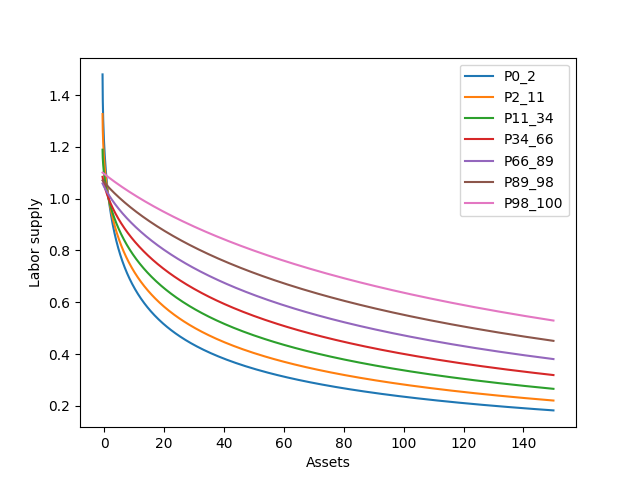
\includegraphics[width=0.45\textwidth]{figures_final/labor_supply_vs_assets.png}
  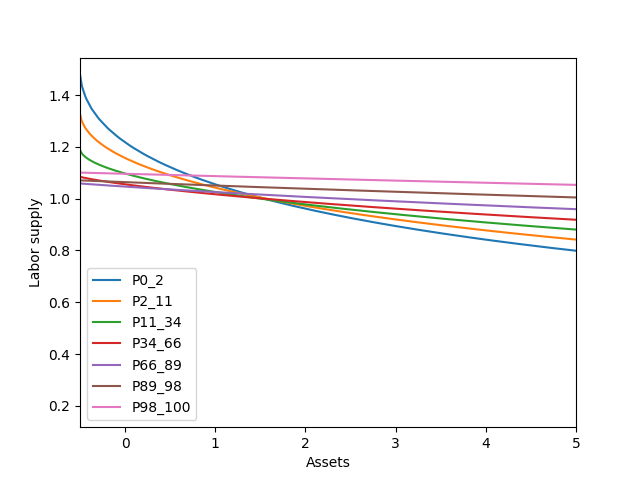
\includegraphics[width=0.45\textwidth]{figures_final/labor_supply_vs_assets_zoomed.png}
  
  \label{fig:LS_PC}

  
   {\footnotesize \textit{Notes:} The left-hand side panel shows it for the full
asset grid, while the right-hand side zooms in on the lower tail of the wealth distribution,
where borrowing constraints bind. \par}

\end{figure}



\begin{figure}[h!]
    \centering
     \caption{Consumption policy function with baseline calibration}
    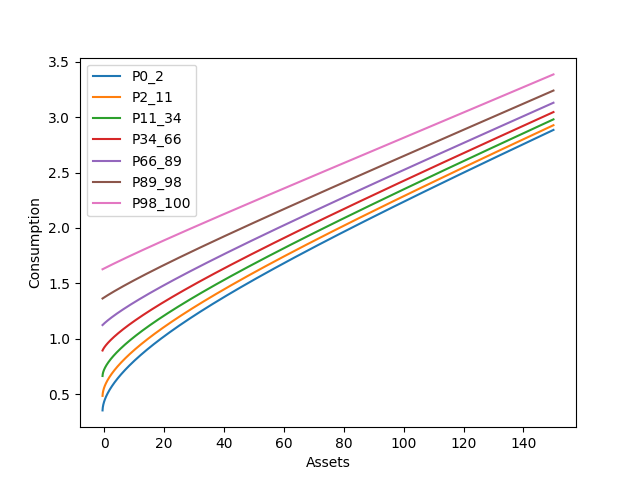
\includegraphics[width=.5\linewidth]{figures_final/consumption_vs_assets.png}
    \label{fig:C_policy}
\end{figure}


\clearpage

\subsection{Policy functions and IRFs across alternative calibrations of the HANK model}\label{A:HANK_PF}

\begin{figure}[h]
  \centering
    \caption{Labor Supply Policy Functions with $\underline{a}=-0.5$ and $\sigma=1$}
  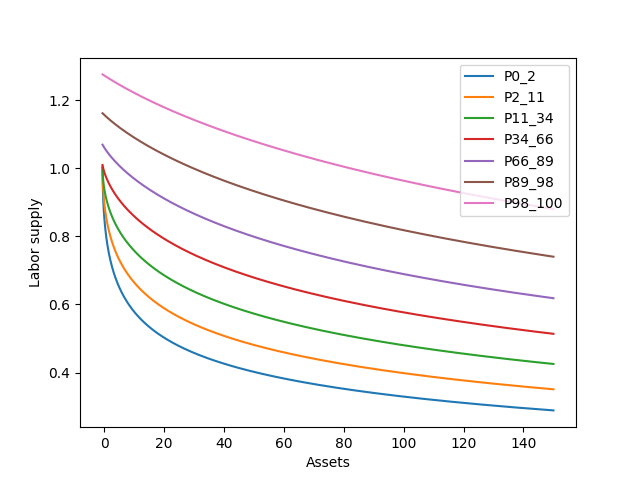
\includegraphics[width=0.45\textwidth]{figures_final/labor_supply_vs_assets_HANK-HetL EIS1.png}
  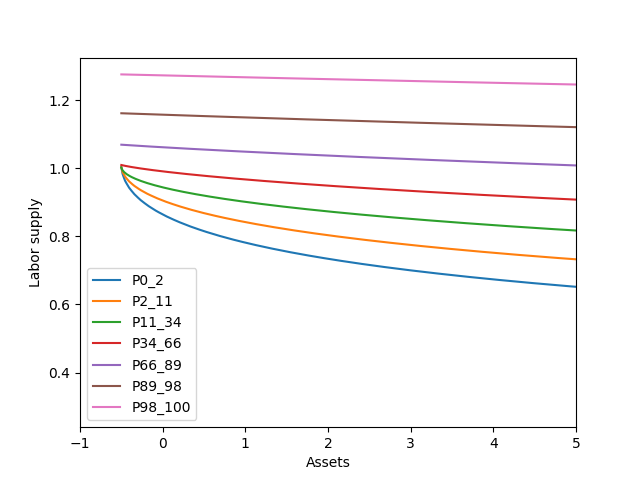
\includegraphics[width=0.45\textwidth]{figures_final/labor_supply_vs_assets_zoomed_HANK-HetL EIS1.png}
  \label{fig:LS_PC_a1_s1}
\end{figure}

\begin{figure}[h!]
    \centering
    \caption{Consumption policy function with $\underline{a}=-0.5$ and $\sigma=1$}
   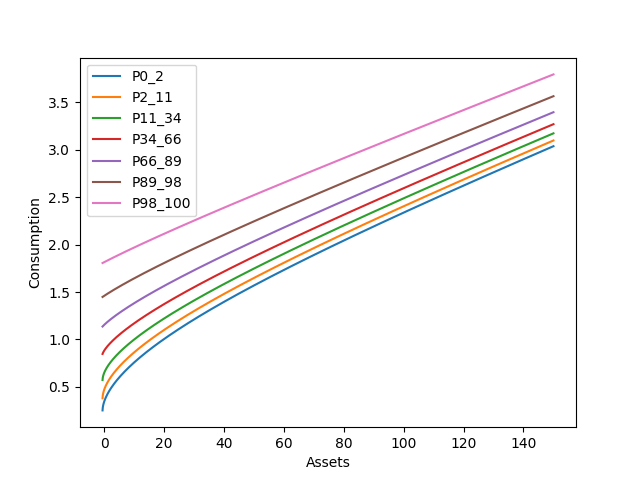
\includegraphics[width=.5\linewidth]{figures_final/consumption_vs_assets_HANK-HetL EIS1.png}
     \label{fig:C_policy_a1_s1}
\end{figure}



\begin{figure}
    \centering
    \caption{Impulse responses to a 25 basis points Monetary Policy Shock with $\underline{a}=-0.5$ and $\sigma=1$}
    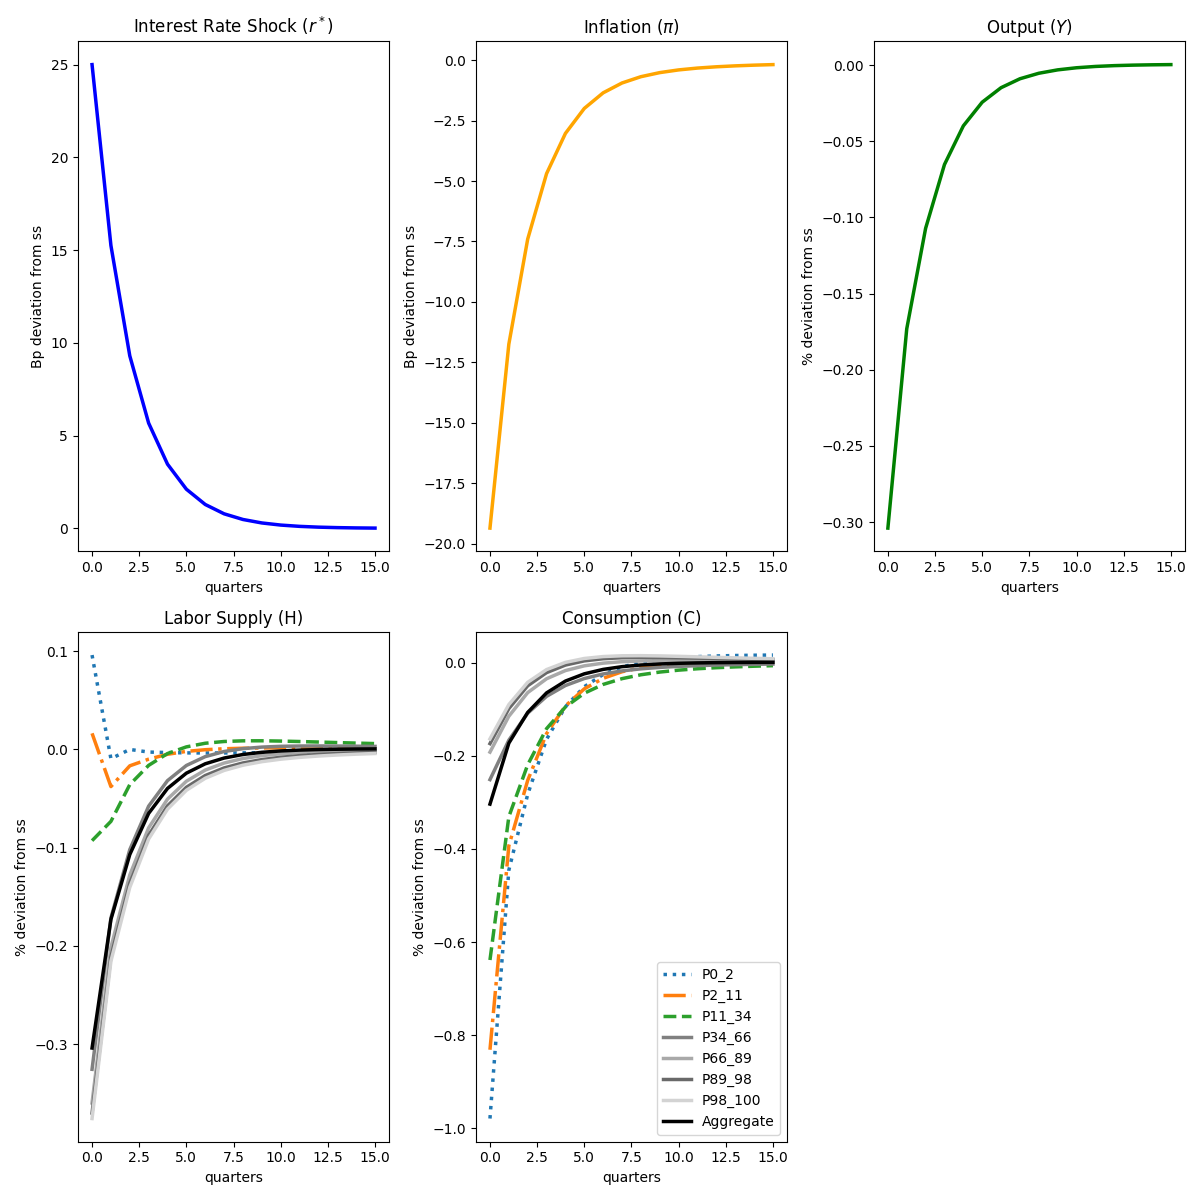
\includegraphics[width=.5\linewidth]{figures_final/IRFs_with_L_and_C_HANK-HetL EIS1.png}
    \label{fig:irfs_a1_s1}
\end{figure}

\begin{figure}[h]
  \centering
  \caption{Labor Supply Policy Functions with $\underline{a}=-0.5$ and $\sigma=0.25$}
  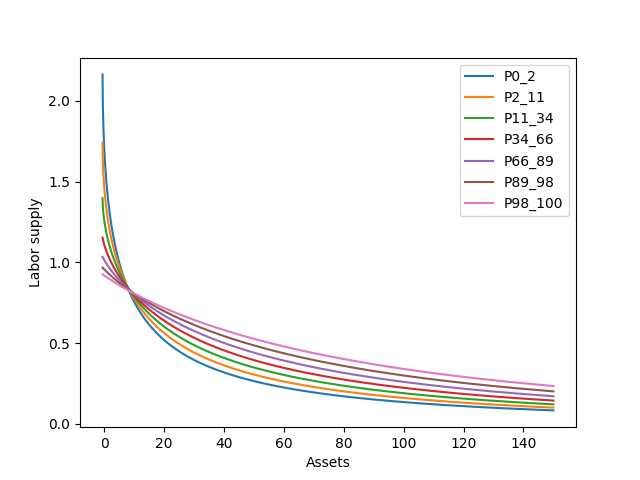
\includegraphics[width=0.45\textwidth]{figures_final/labor_supply_vs_assets_HANK-HetL EIS025.png}
  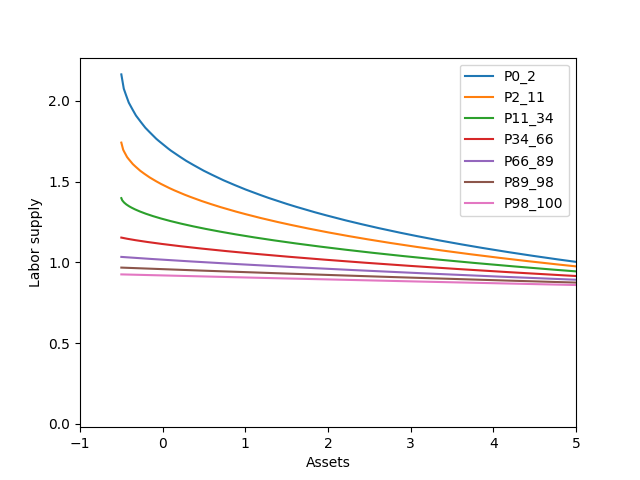
\includegraphics[width=0.45\textwidth]{figures_final/labor_supply_vs_assets_zoomed_HANK-HetL EIS025.png}
  \label{fig:LS_PC_a1_s025}
\end{figure}

\begin{figure}[h!]
    \centering
    \caption{Consumption policy function with $\underline{a}=-0.5$ and $\sigma=0.25$}
    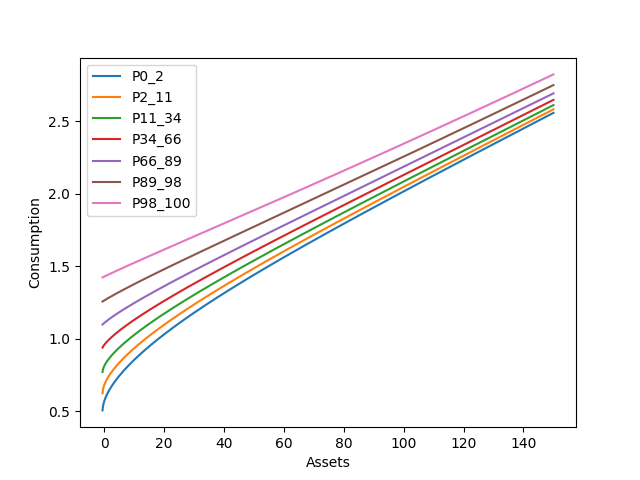
\includegraphics[width=.5\linewidth]{figures_final/consumption_vs_assets_HANK-HetL EIS025.png}
    \label{fig:C_policy_a1_s025}
\end{figure}



\begin{figure}
    \centering
    \caption{Impulse responses to a 25 basis points Monetary Policy Shock with $\underline{a}=-0.5$ and $\sigma=0.25$}
    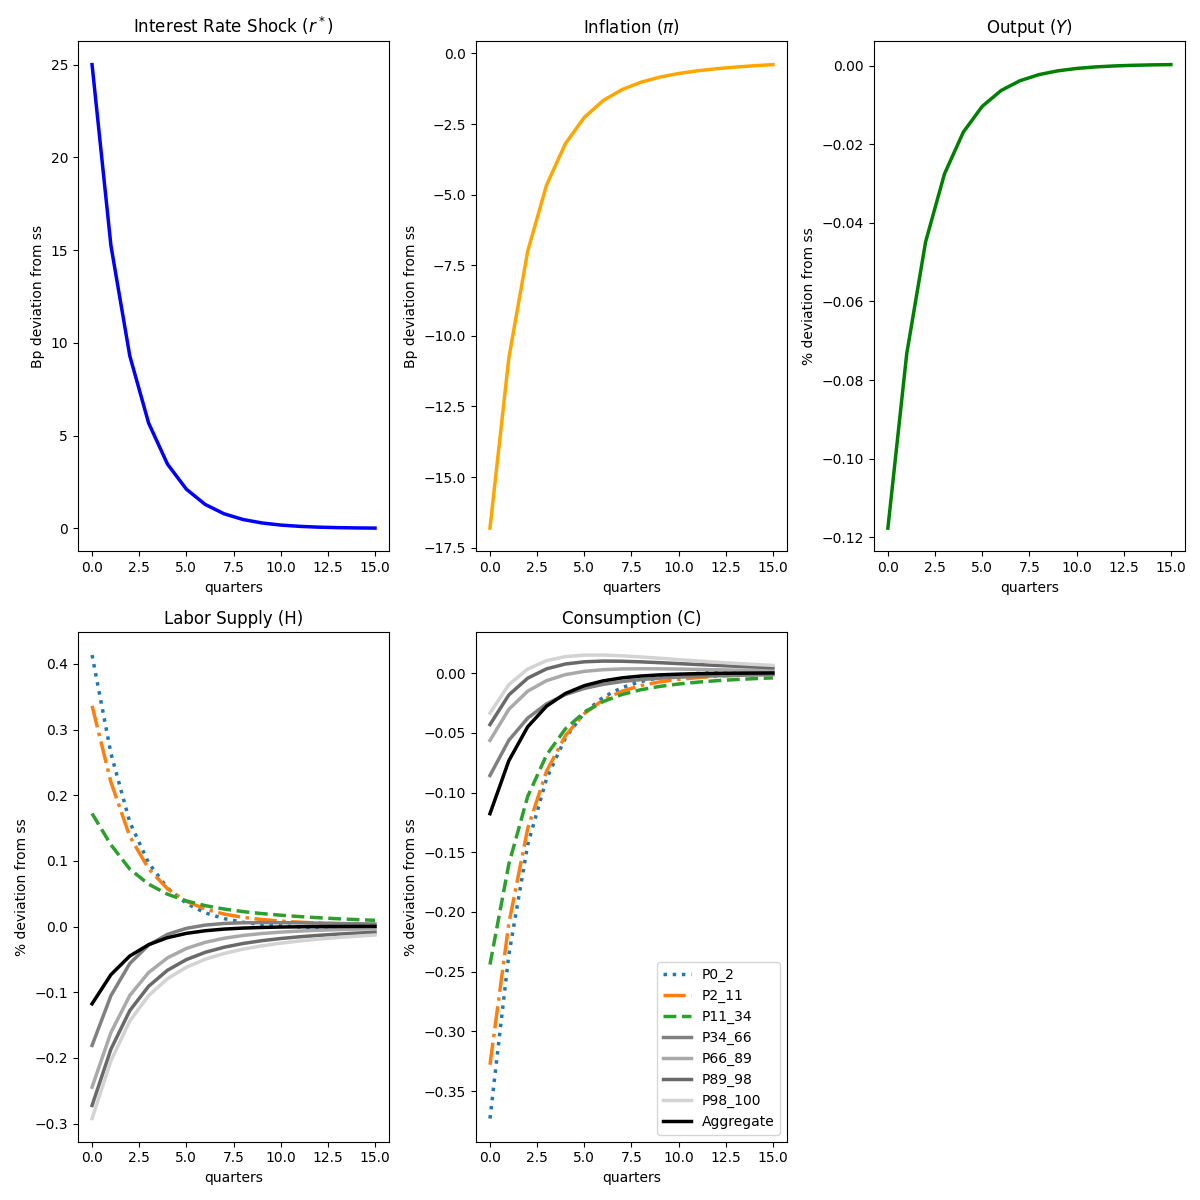
\includegraphics[width=.5\linewidth]{figures_final/IRFs_with_L_and_C_HANK-HetL EIS025.png}
    \label{fig:irfs_a1_s025}
\end{figure}


\begin{figure}[h]
  \centering
  \caption{Labor Supply Policy Functions with $\underline{a}=0$ and $\sigma=1$}
  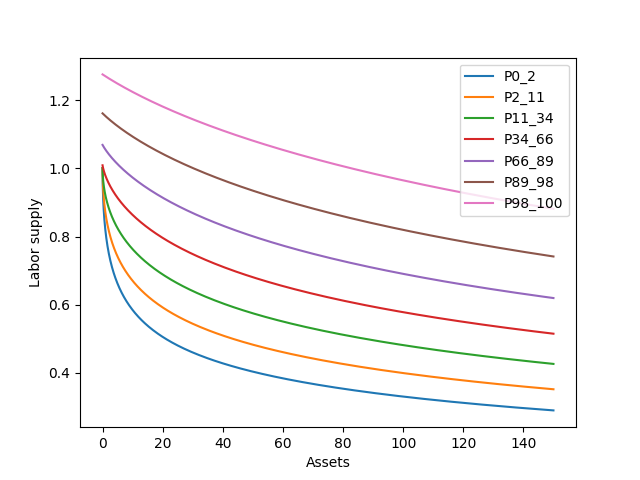
\includegraphics[width=0.45\textwidth]{figures_final/labor_supply_vs_assets_HANK-HetL EIS1 a0.png}
  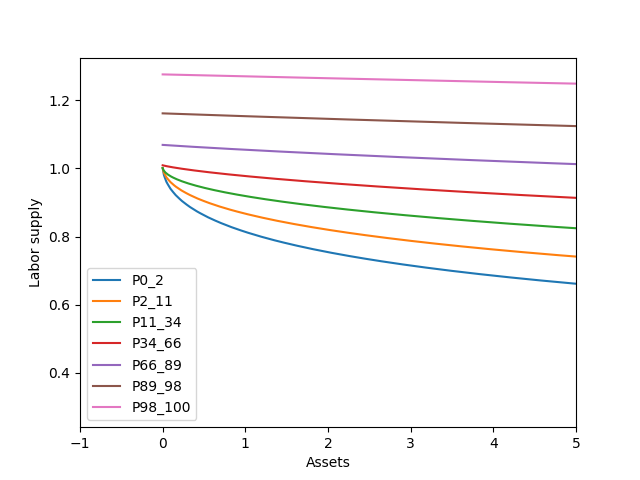
\includegraphics[width=0.45\textwidth]{figures_final/labor_supply_vs_assets_zoomed_HANK-HetL EIS1 a0.png}
  \label{fig:LS_PC_a0_s1}
\end{figure}

\begin{figure}[h!]
    \centering
    \caption{Consumption policy function with $\underline{a}=0$ and $\sigma=1$}
    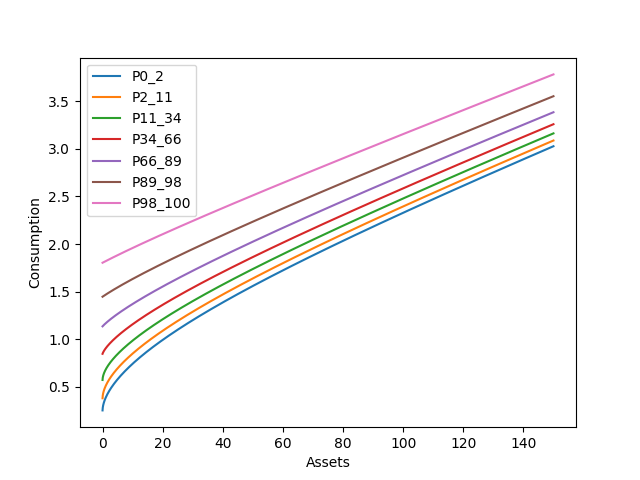
\includegraphics[width=0.5\linewidth]{figures_final/consumption_vs_assets_HANK-HetL EIS1 a0.png}
    \label{fig:C_policy_a0_s1}
\end{figure}



\begin{figure}
    \centering
    \caption{Impulse responses to a 25 basis points Monetary Policy Shock with $\underline{a}=0$ and $\sigma=1$}
    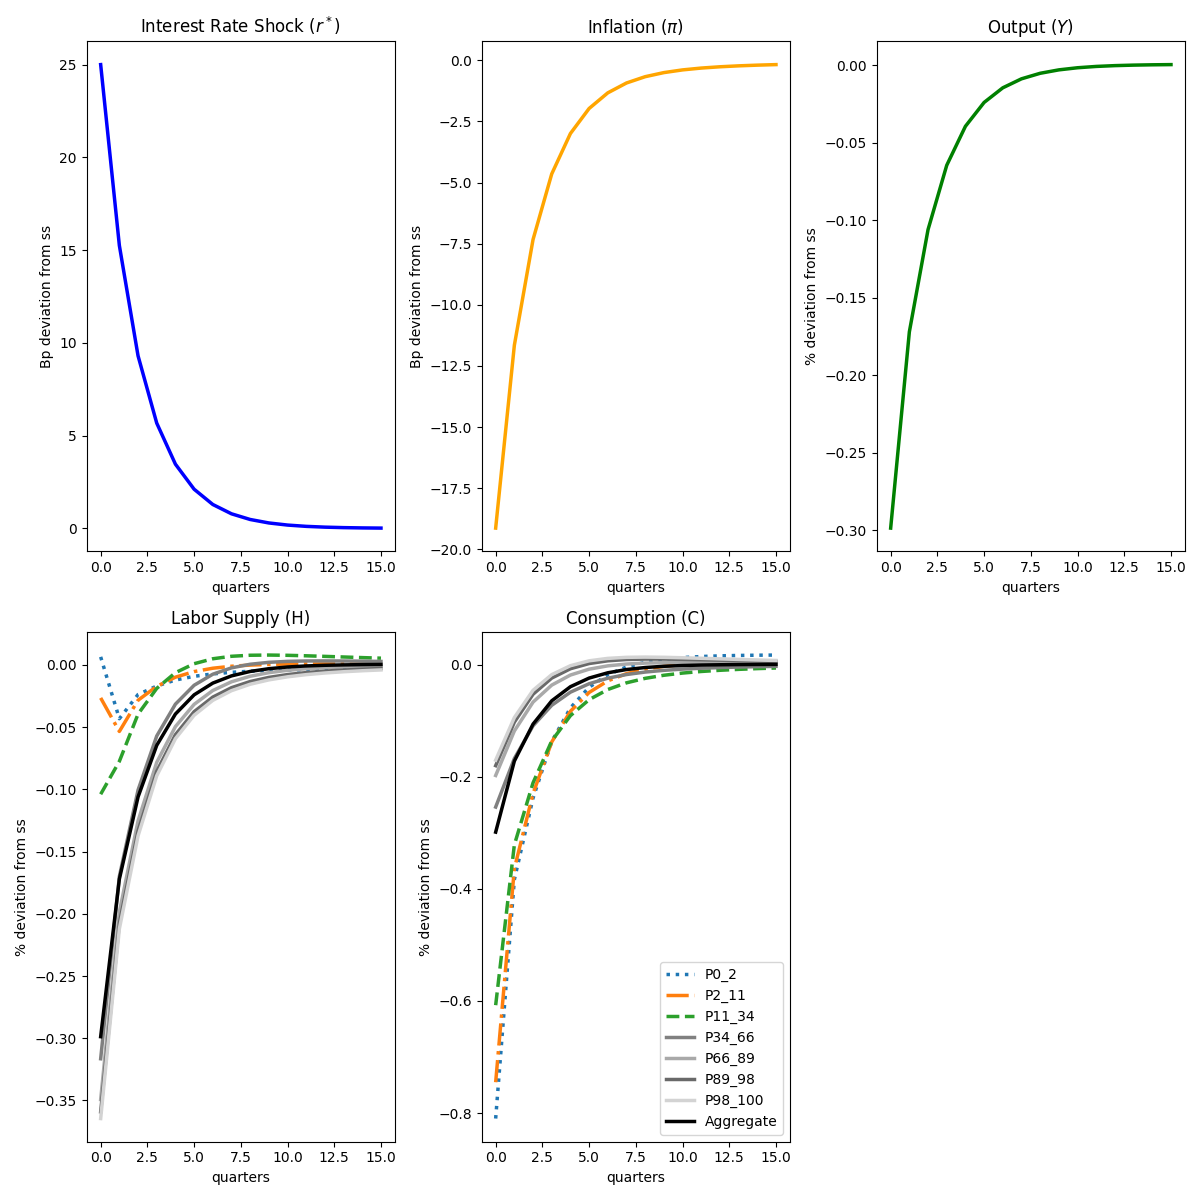
\includegraphics[width=.5\linewidth]{figures_final/IRFs_with_L_and_C_HANK-HetL EIS1 a0.png}
    \label{fig:irfs_a0_s1}
\end{figure}

\begin{figure}[h]
  \centering
  \caption{Labor Supply Policy Functions with $\underline{a}=0$ and $\sigma=0.5$}
  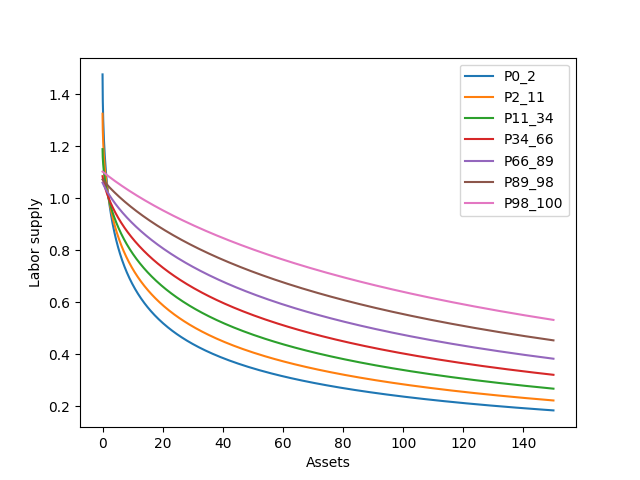
\includegraphics[width=0.45\textwidth]{figures_final/labor_supply_vs_assets_HANK-HetL a0.png}
  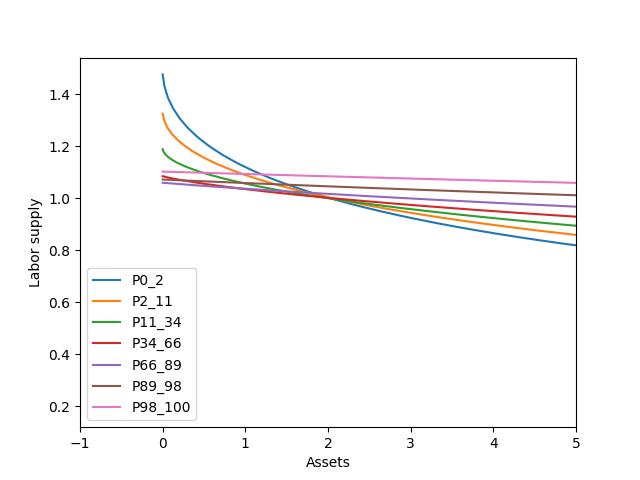
\includegraphics[width=0.45\textwidth]{figures_final/labor_supply_vs_assets_zoomed_HANK-HetL a0.png}
  \label{fig:LS_PC_a0_s05}
\end{figure}

\begin{figure}[h!]
    \centering
    \caption{Consumption policy function with $\underline{a}=0$ and $\sigma=0.5$}
    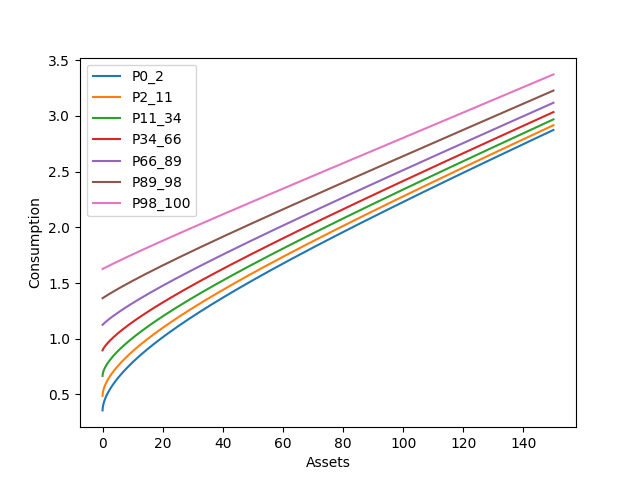
\includegraphics[width=.5\linewidth]{figures_final/consumption_vs_assets_HANK-HetL a0.png}
    \label{fig:C_policy_a0_s05}
\end{figure}



\begin{figure}
    \centering
    \caption{Impulse responses to a 25 basis points Monetary Policy Shock with $\underline{a}=0$ and $\sigma=0.5$}
    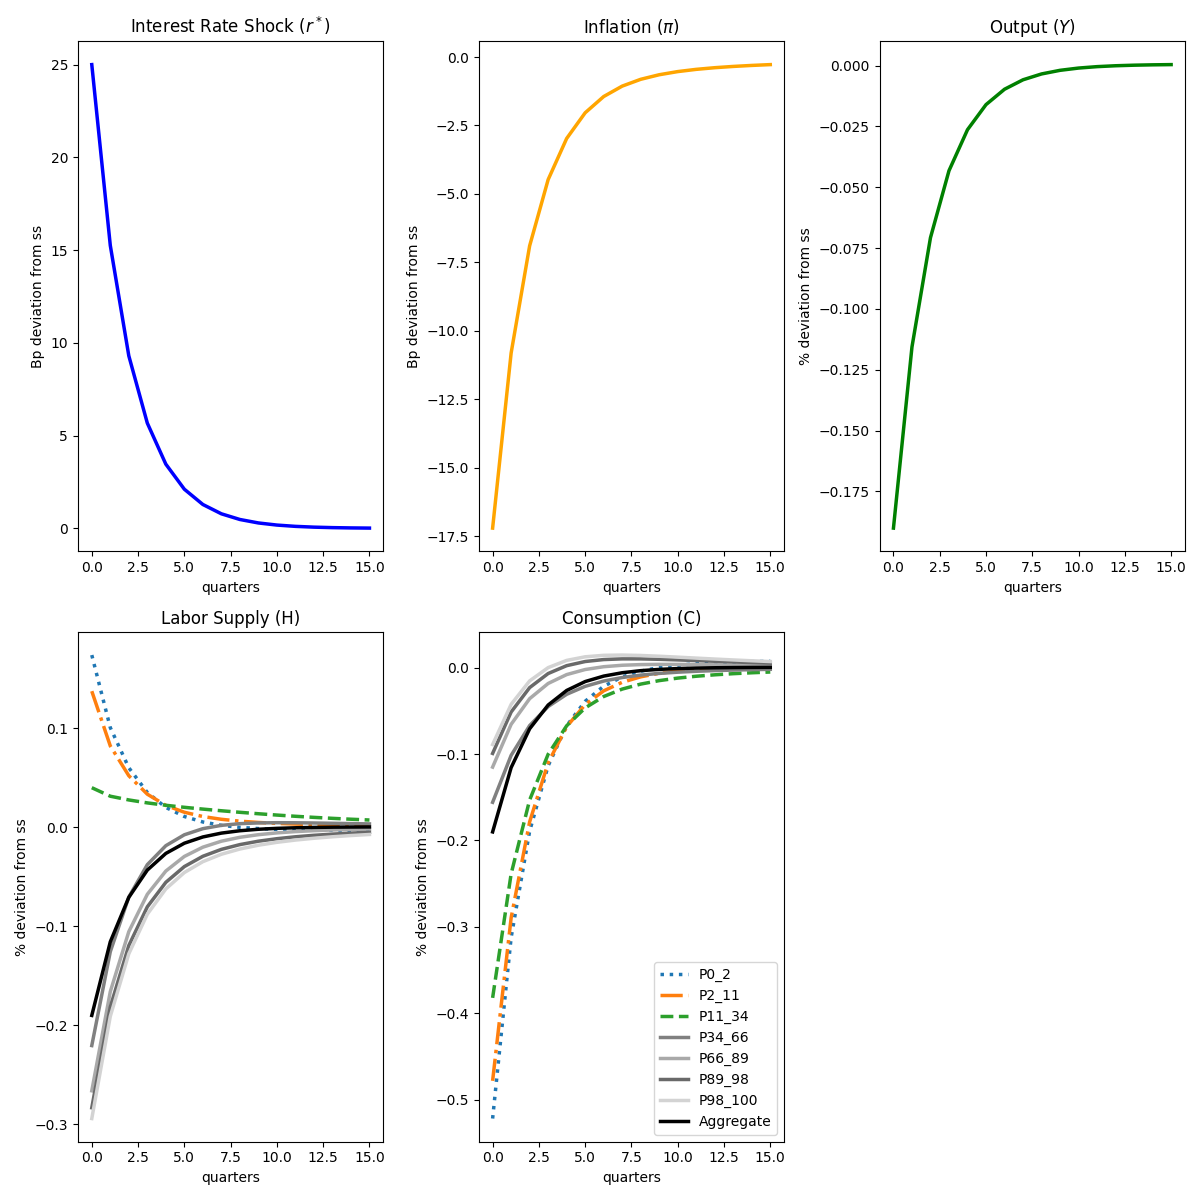
\includegraphics[width=.5\linewidth]{figures_final/IRFs_with_L_and_C_HANK-HetL a0.png}
    \label{fig:irfs_a0_s05}
\end{figure}

\begin{figure}[h]
  \centering
  \caption{Labor Supply Policy Functions with $\underline{a}=0$ and $\sigma=0.25$}
  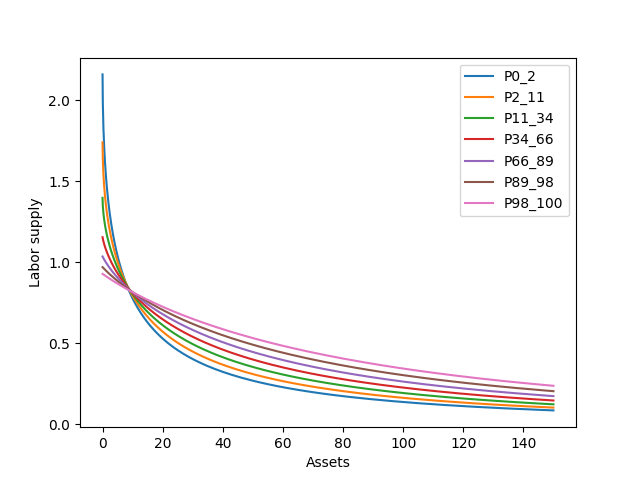
\includegraphics[width=0.45\textwidth]{figures_final/labor_supply_vs_assets_HANK-HetL EIS025 a0.png}
  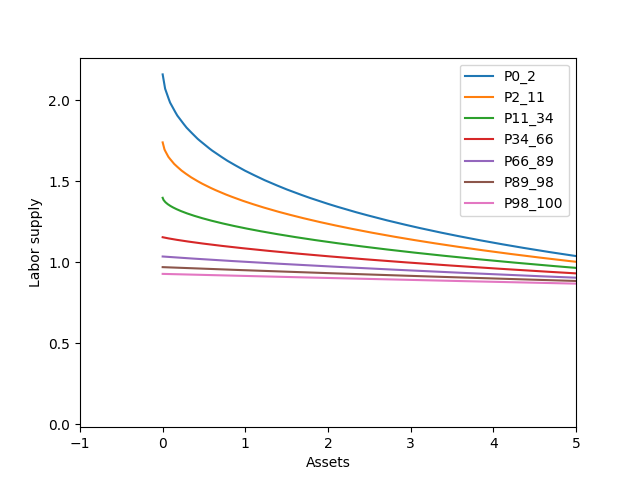
\includegraphics[width=0.45\textwidth]{figures_final/labor_supply_vs_assets_zoomed_HANK-HetL EIS025 a0.png}
  \label{fig:LS_PC_a0_s025}
\end{figure}

\begin{figure}[h!]
    \centering
    \caption{Consumption policy function with $\underline{a}=0$ and $\sigma=0.25$}
    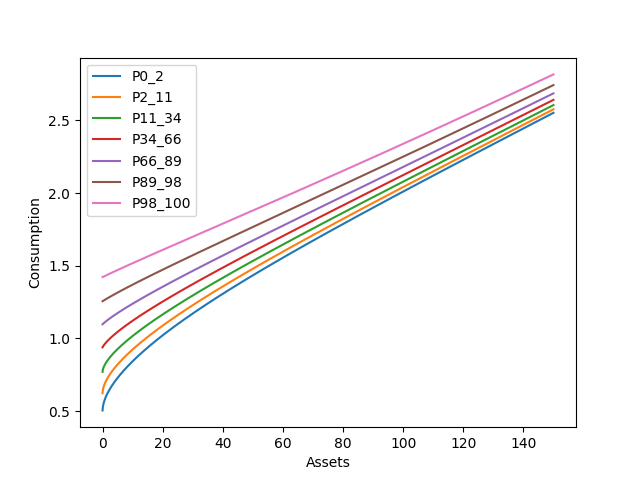
\includegraphics[width=.5\linewidth]{figures_final/consumption_vs_assets_HANK-HetL EIS025 a0.png}
    \label{fig:C_policy_a0_s025}
\end{figure}



\begin{figure}
    \centering
    \caption{Impulse responses to a 25 basis points Monetary Policy Shock with $\underline{a}=0$ and $\sigma=0.25$}
    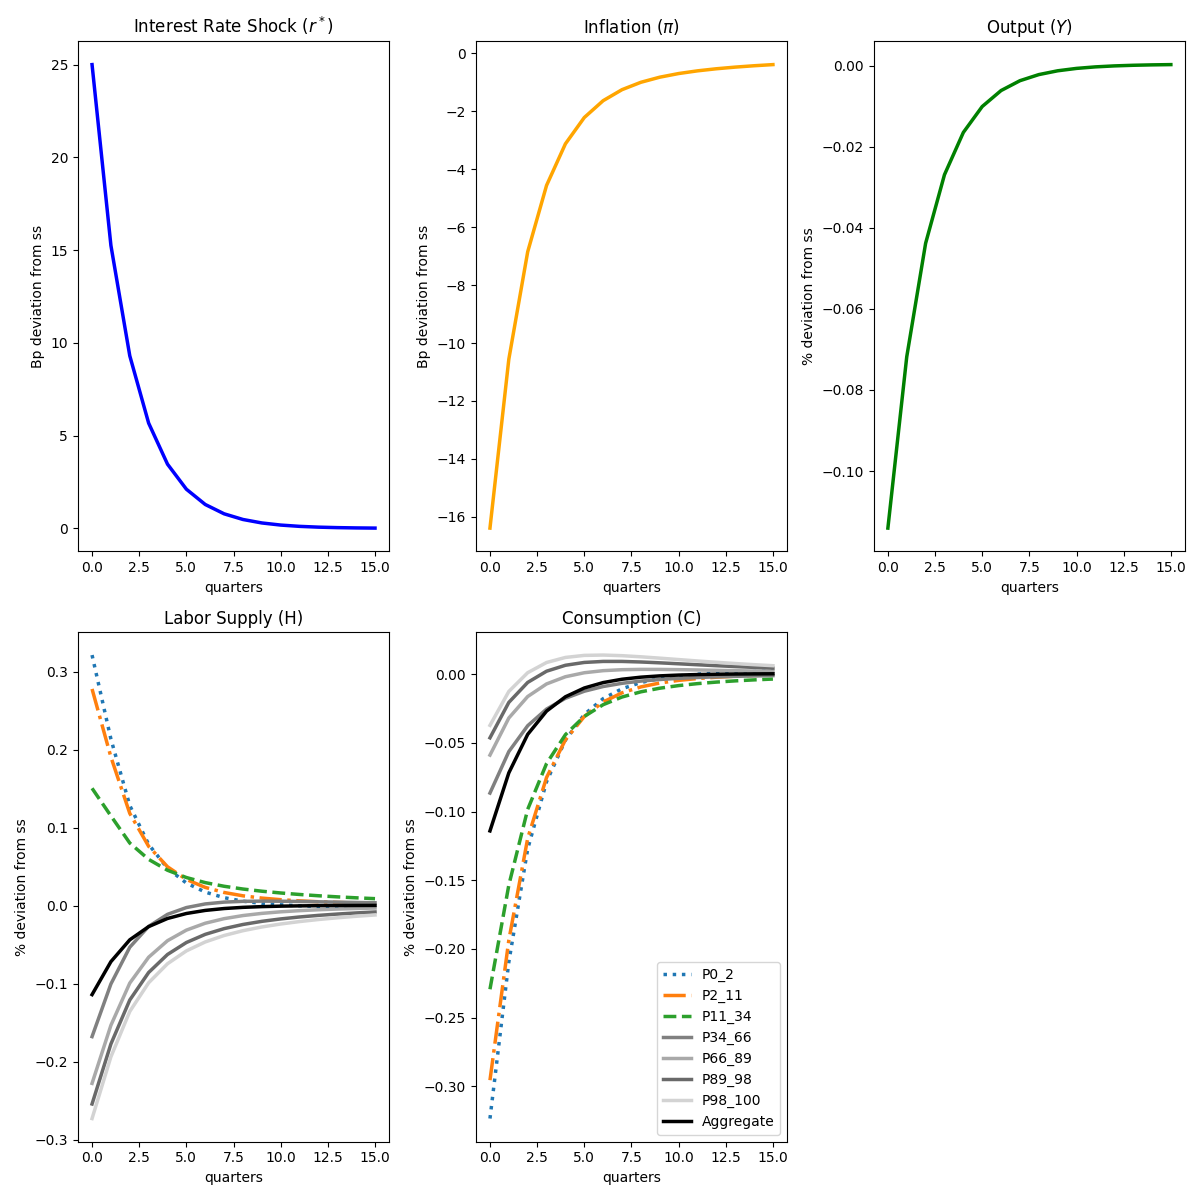
\includegraphics[width=.5\linewidth]{figures_final/IRFs_with_L_and_C_HANK-HetL EIS025 a0.png}
    \label{fig:irfs_a0_s025}
\end{figure}

\clearpage

\subsection{IRFs decompositions HANK}\label{A:Irfs_deco}

\begin{figure}[h!]
  \centering
  \caption{Decomposition of consumption Response in HANK. }
  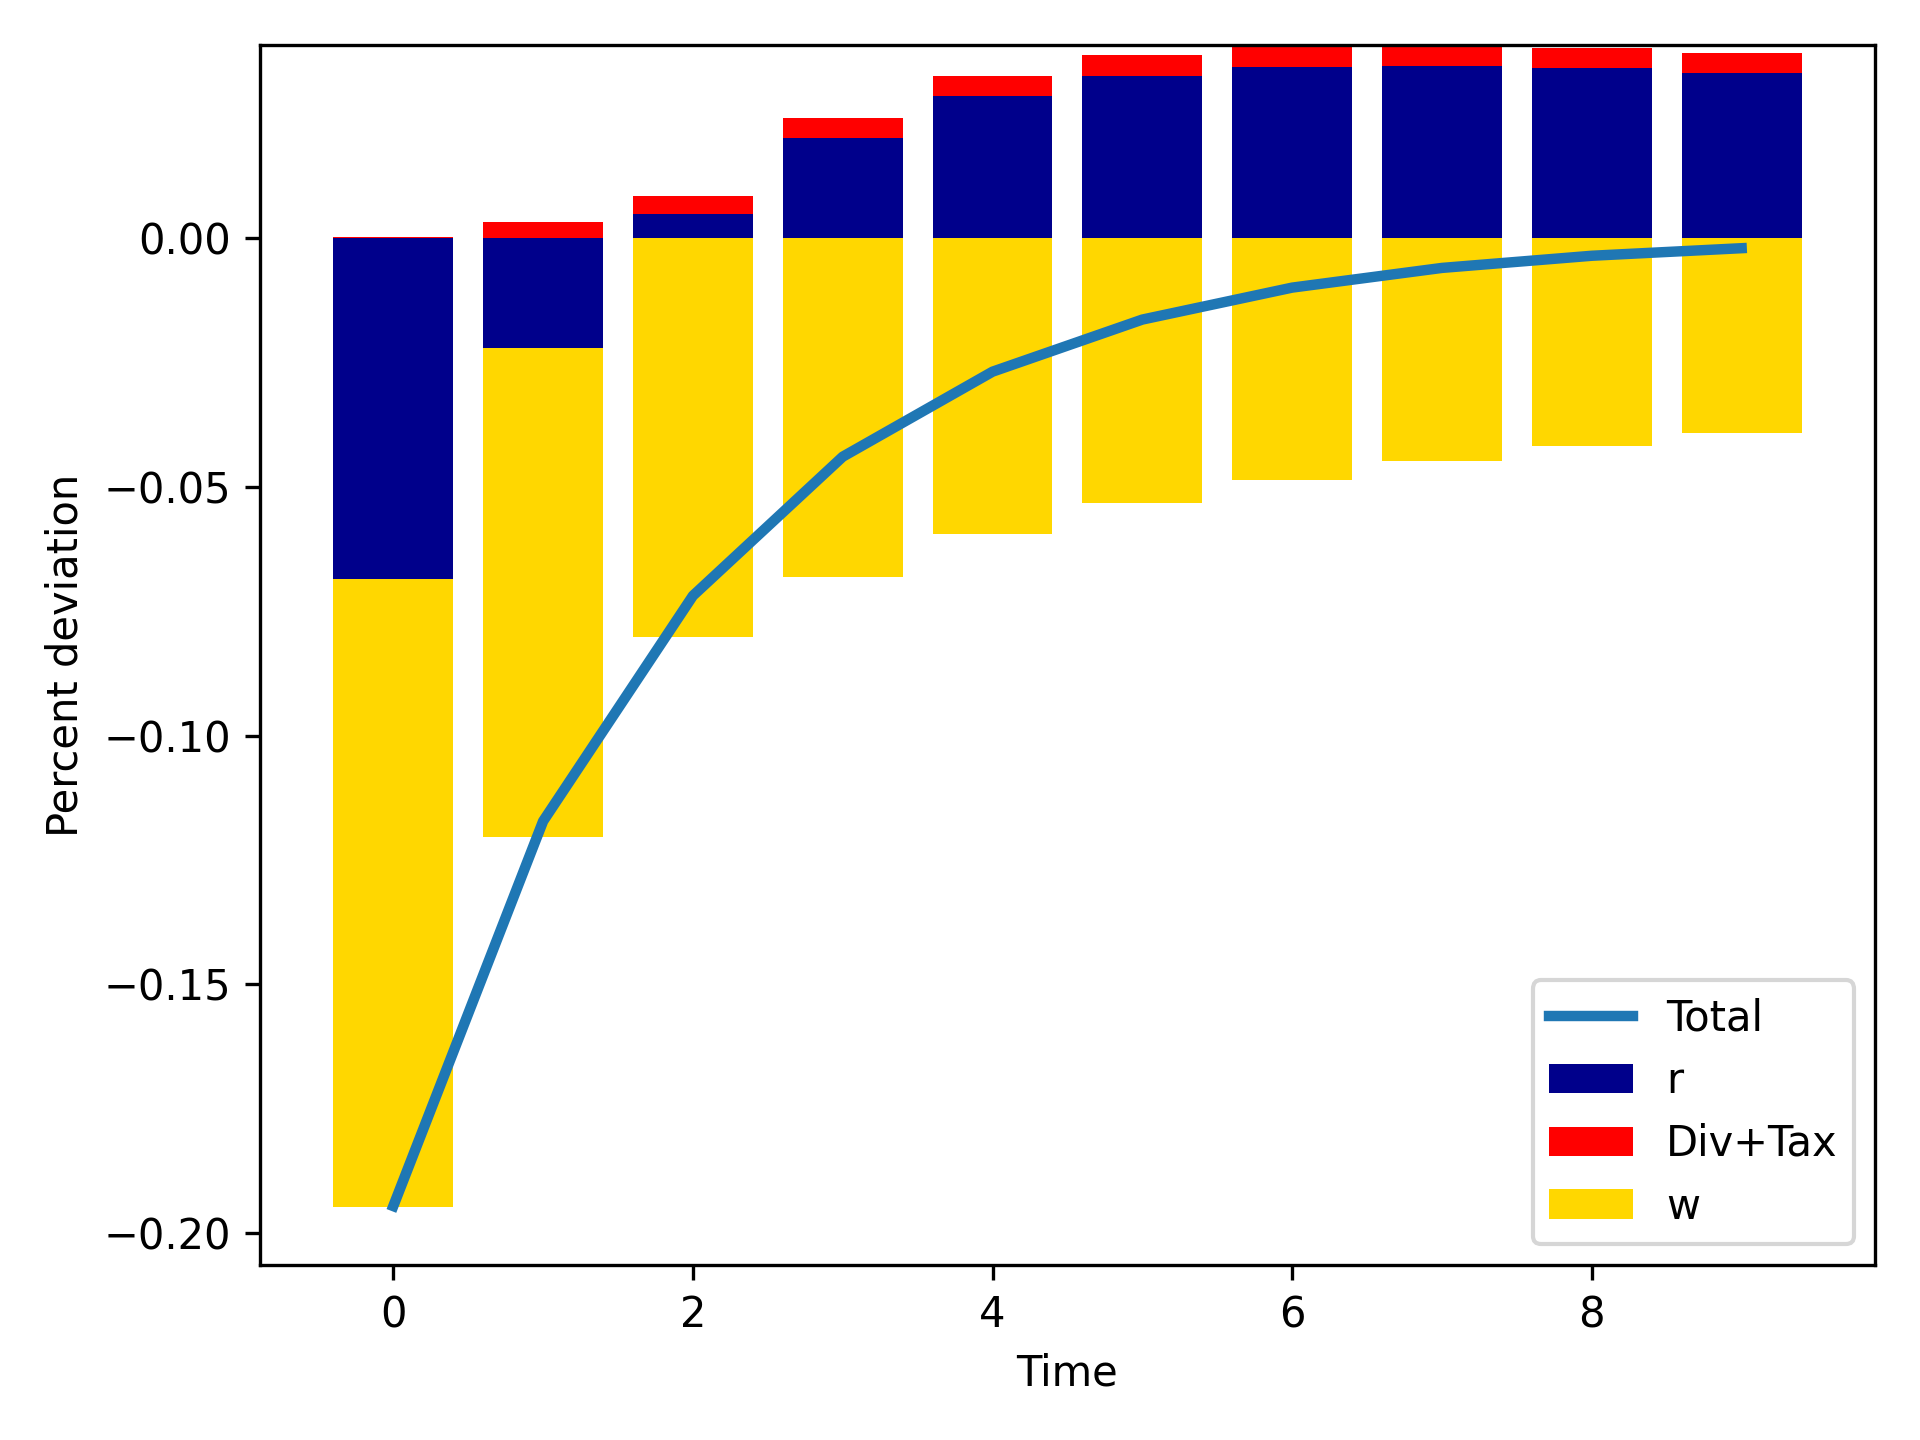
\includegraphics[width=0.8\textwidth]{figures_final/HANK_HetL_decomp_C_comb.png}
  \label{fig:hetl_cons_decomp}

     {\footnotesize \textit{Notes:} Percent deviation in aggregate consumption from steady state, decomposed into marginal channels: interest rate, dividends, taxes, and wages. \par}
\end{figure}



\begin{figure}[h!]
  \centering
  \caption{Decomposition of consumption Responses by Income Bin --- HANK.}
  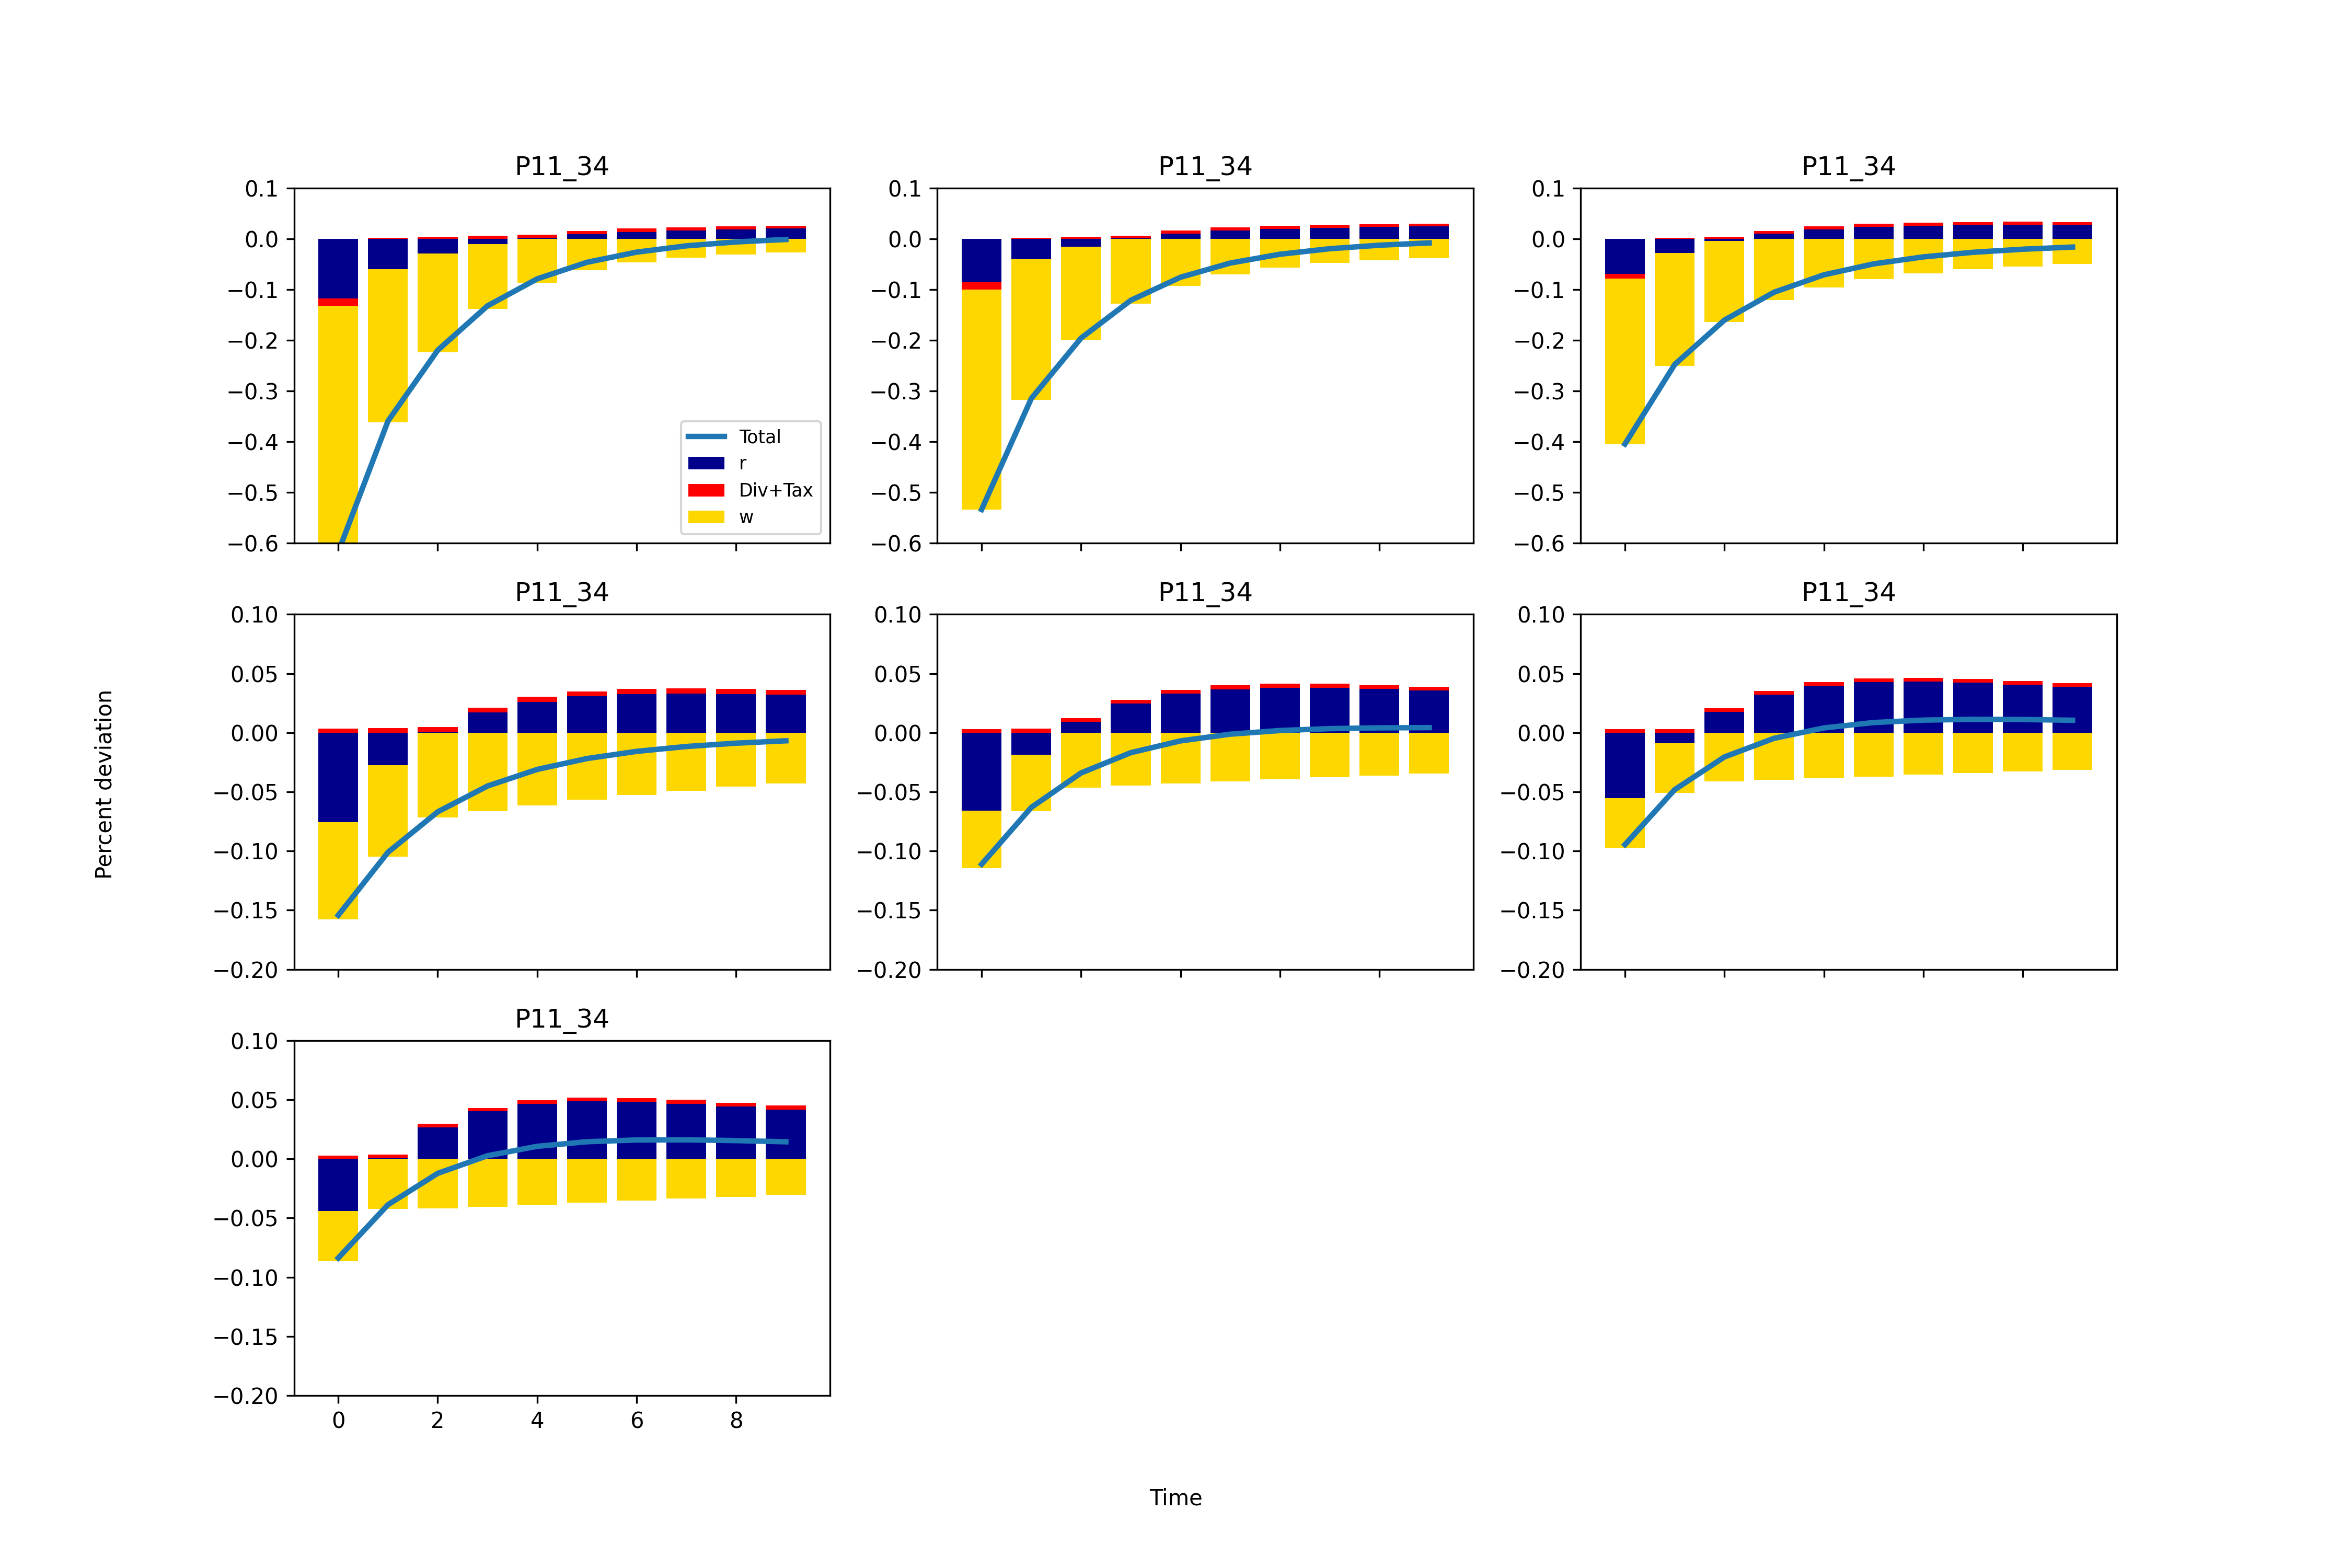
\includegraphics[width=\textwidth]{figures_final/HANK_HetL_decomp_bins_C_comb.png}
  \label{fig:hetl_cons_bins}

  {\footnotesize \textit{Notes:} Each panel shows percent deviation in consumption from steady state, decomposed into marginal channels: interest rate, wages, dividends, and taxes. \par}

\end{figure}




\clearpage

\subsection{HANK vs HANK-HomL}\label{A:HANKvsHOML}

\begin{figure}[h!]
  \centering
  \caption{Impact response of labor supply across income states in HANK vs the aggregate impact response in HANK-HomL}
  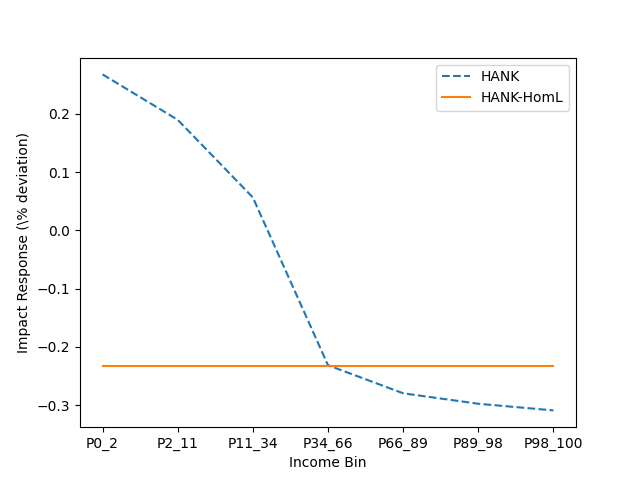
\includegraphics[width=\textwidth]{figures_final/impact_labor_supply_hom_vs_het.png}
  \label{fig:impact_H_eis}
\end{figure}

\begin{figure}[h!]
  \centering
  \caption{Direct vs indirect effects of monetary policy on aggregate consumption in HANK vs HANK-HomL for baseline $\sigma$.}
  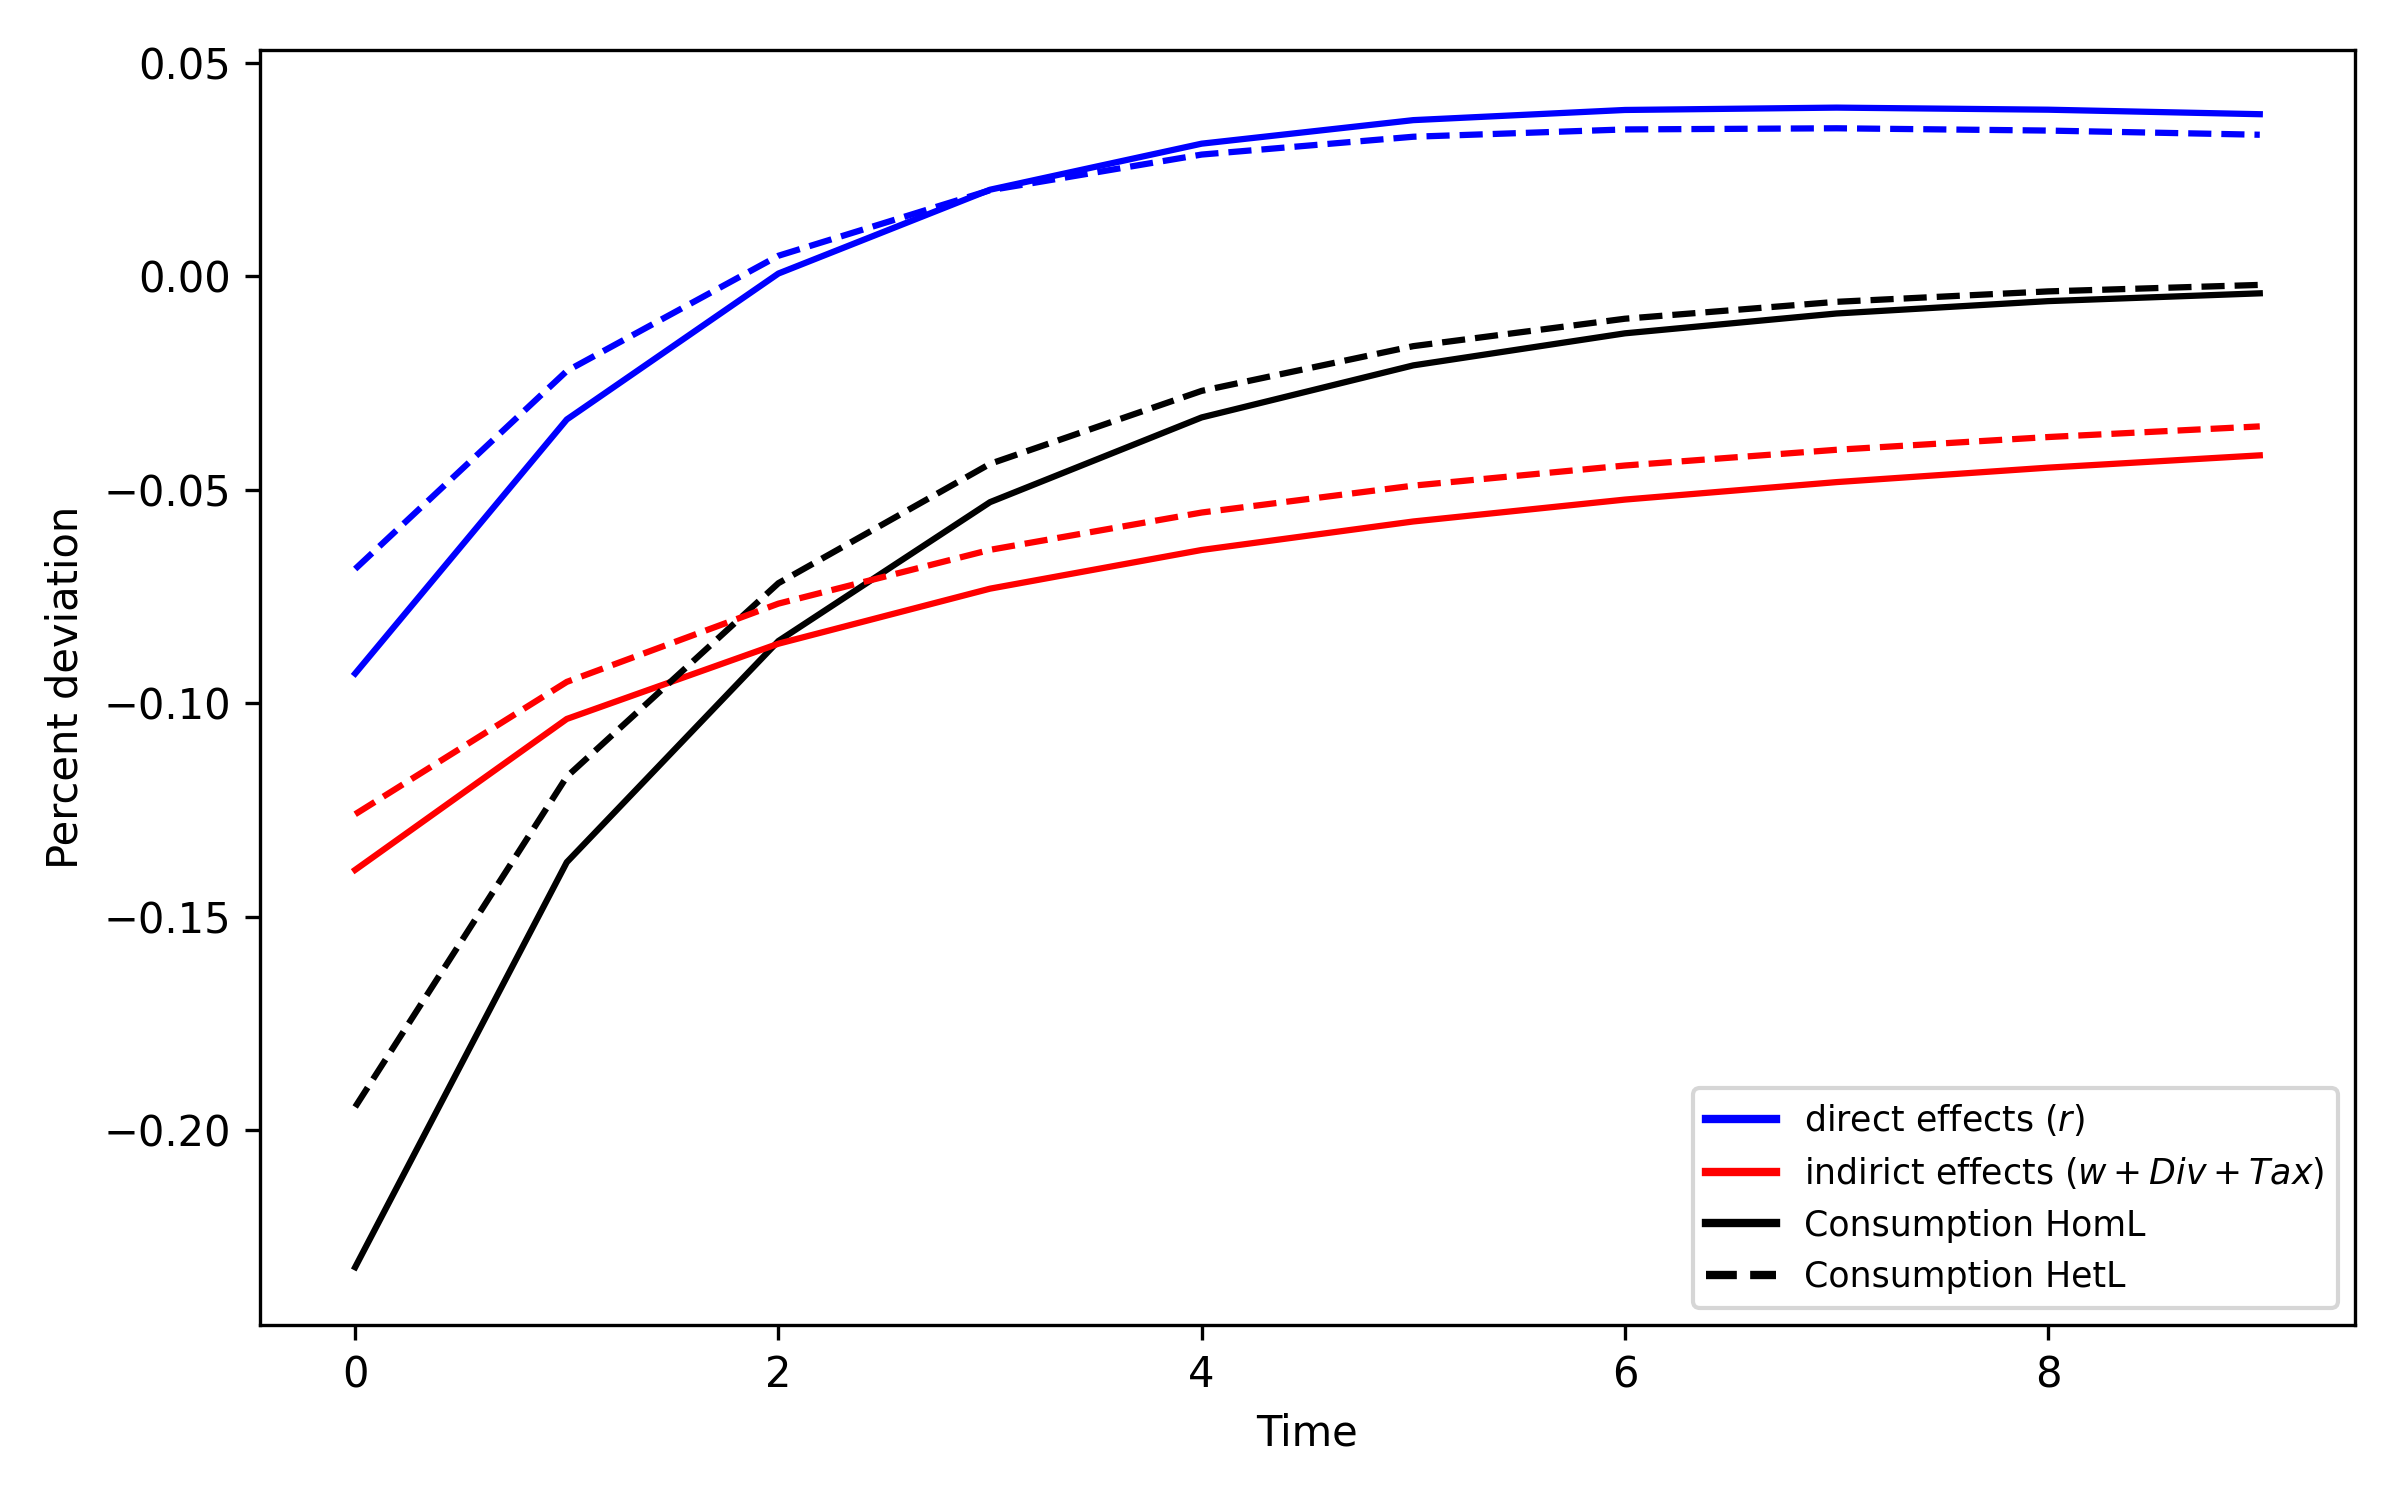
\includegraphics[width=\textwidth]{figures_final/HANK_direct_vs_indirect_C_simple.png}
  \label{fig:dir_vs_indir}
\end{figure}

\clearpage

Table \ref{tab:HANK_calib_comp} in the main text highlights that accounting for heterogeneity in labor supply has quantitatively significant implications, notably lowering the economy's average MPC. This, in turn, affects the transmission of monetary policy.
To illustrate this we compare here the dynamic responses to a contractionary monetary policy shock in the HANK and HANK-HomL models. Figure \ref{fig:core_irfs} reports aggregate impulse responses for interest rates, inflation, output, wages, dividends, and the share of hand-to-mouth households.
Aggregate price and dividend dynamics are broadly similar across models, as expected given their identical firm and policy structure. However, two notable differences emerge. First, the HTM share rises more and remains elevated longer in HANK. Here we measure HTM as the fraction of households at the borrowing limit \(a=\underline{a}\). This pattern is consistent with households smoothing the contraction by dissaving/borrowing, which shifts more mass to the constraint even as low-income households increase labor effort. Second, aggregate consumption declines by 16\% less on impact in HANK compared to HANK-HomL. This muted response reflects the additional margin of adjustment provided by heterogeneous labor supply, which allows low-income households to buffer shocks through work effort. We explore the distributional responses that drive this result next.

The main-text comparison calibrates HANK-HomL to match the impact response of the median agent’s hours in HANK. As a robustness check, we alternatively choose the EIS in HANK-HomL to match the impact response (period 0) of aggregate labor $L$ in the corresponding HANK calibration, and then recompute the sacrifice ratios.

\begin{table}[h!]
\centering
\begin{tabular}{lcc}
\toprule
 & HANK-HomL (match agg $L$) & HANK \\
\midrule
Low $\sigma$ & 1.02 & 0.67 \\
Baseline $\sigma$ & 1.08 & 1.07 \\
High $\sigma$ & 1.52 & 1.50 \\
\bottomrule
\end{tabular}
\caption{Sacrifice ratios under an alternative comparability criterion. In this robustness exercise, we recalibrate HANK-HomL by choosing its EIS to match the impact response (period 0) of aggregate labor $L$ in the corresponding HANK calibration. Sacrifice ratios are computed as in Table~\ref{tab:sacrifice_ratios} (cumulative output loss divided by cumulative inflation decline over the first four quarters after the shock).}
\label{tab:sacrifice_ratios_aggL}
\end{table}

Figure \ref{fig:L_bins_irfs} shows that, by construction, labor supply responses are almost identical for the median agent type (34--66\%). At the bottom of the distribution, agents increase their labor supply, consistent with our empirical evidence. In contrast, upper-middle and top-income households reduce their labor supply more in the HANK model compared to HANK-HomL. This highlights that the left tail of the labor supply distribution is responsible for the muted amplification of monetary policy on aggregate demand. 
Figure \ref{fig:C_bins_irfs} shows how these labor responses translate into individual consumption dynamics. The consumption decline is most severe at the bottom of the distribution in both models, but the drop is smaller and less persistent in the HANK model. At the top of the distribution, consumption responses are very similar across models.

Another way to quantify the role of different households across the income distribution in shaping the aggregate effects of monetary policy is to compute their respective contributions to the overall impact on consumption and labor supply, measured in basis point deviations. Figure \ref{fig:contribution} presents the results.




\begin{figure}[h!]
  \centering
  \caption{Impulse Responses of Core Macroeconomic Variables: HANK-HomL vs HANK}
  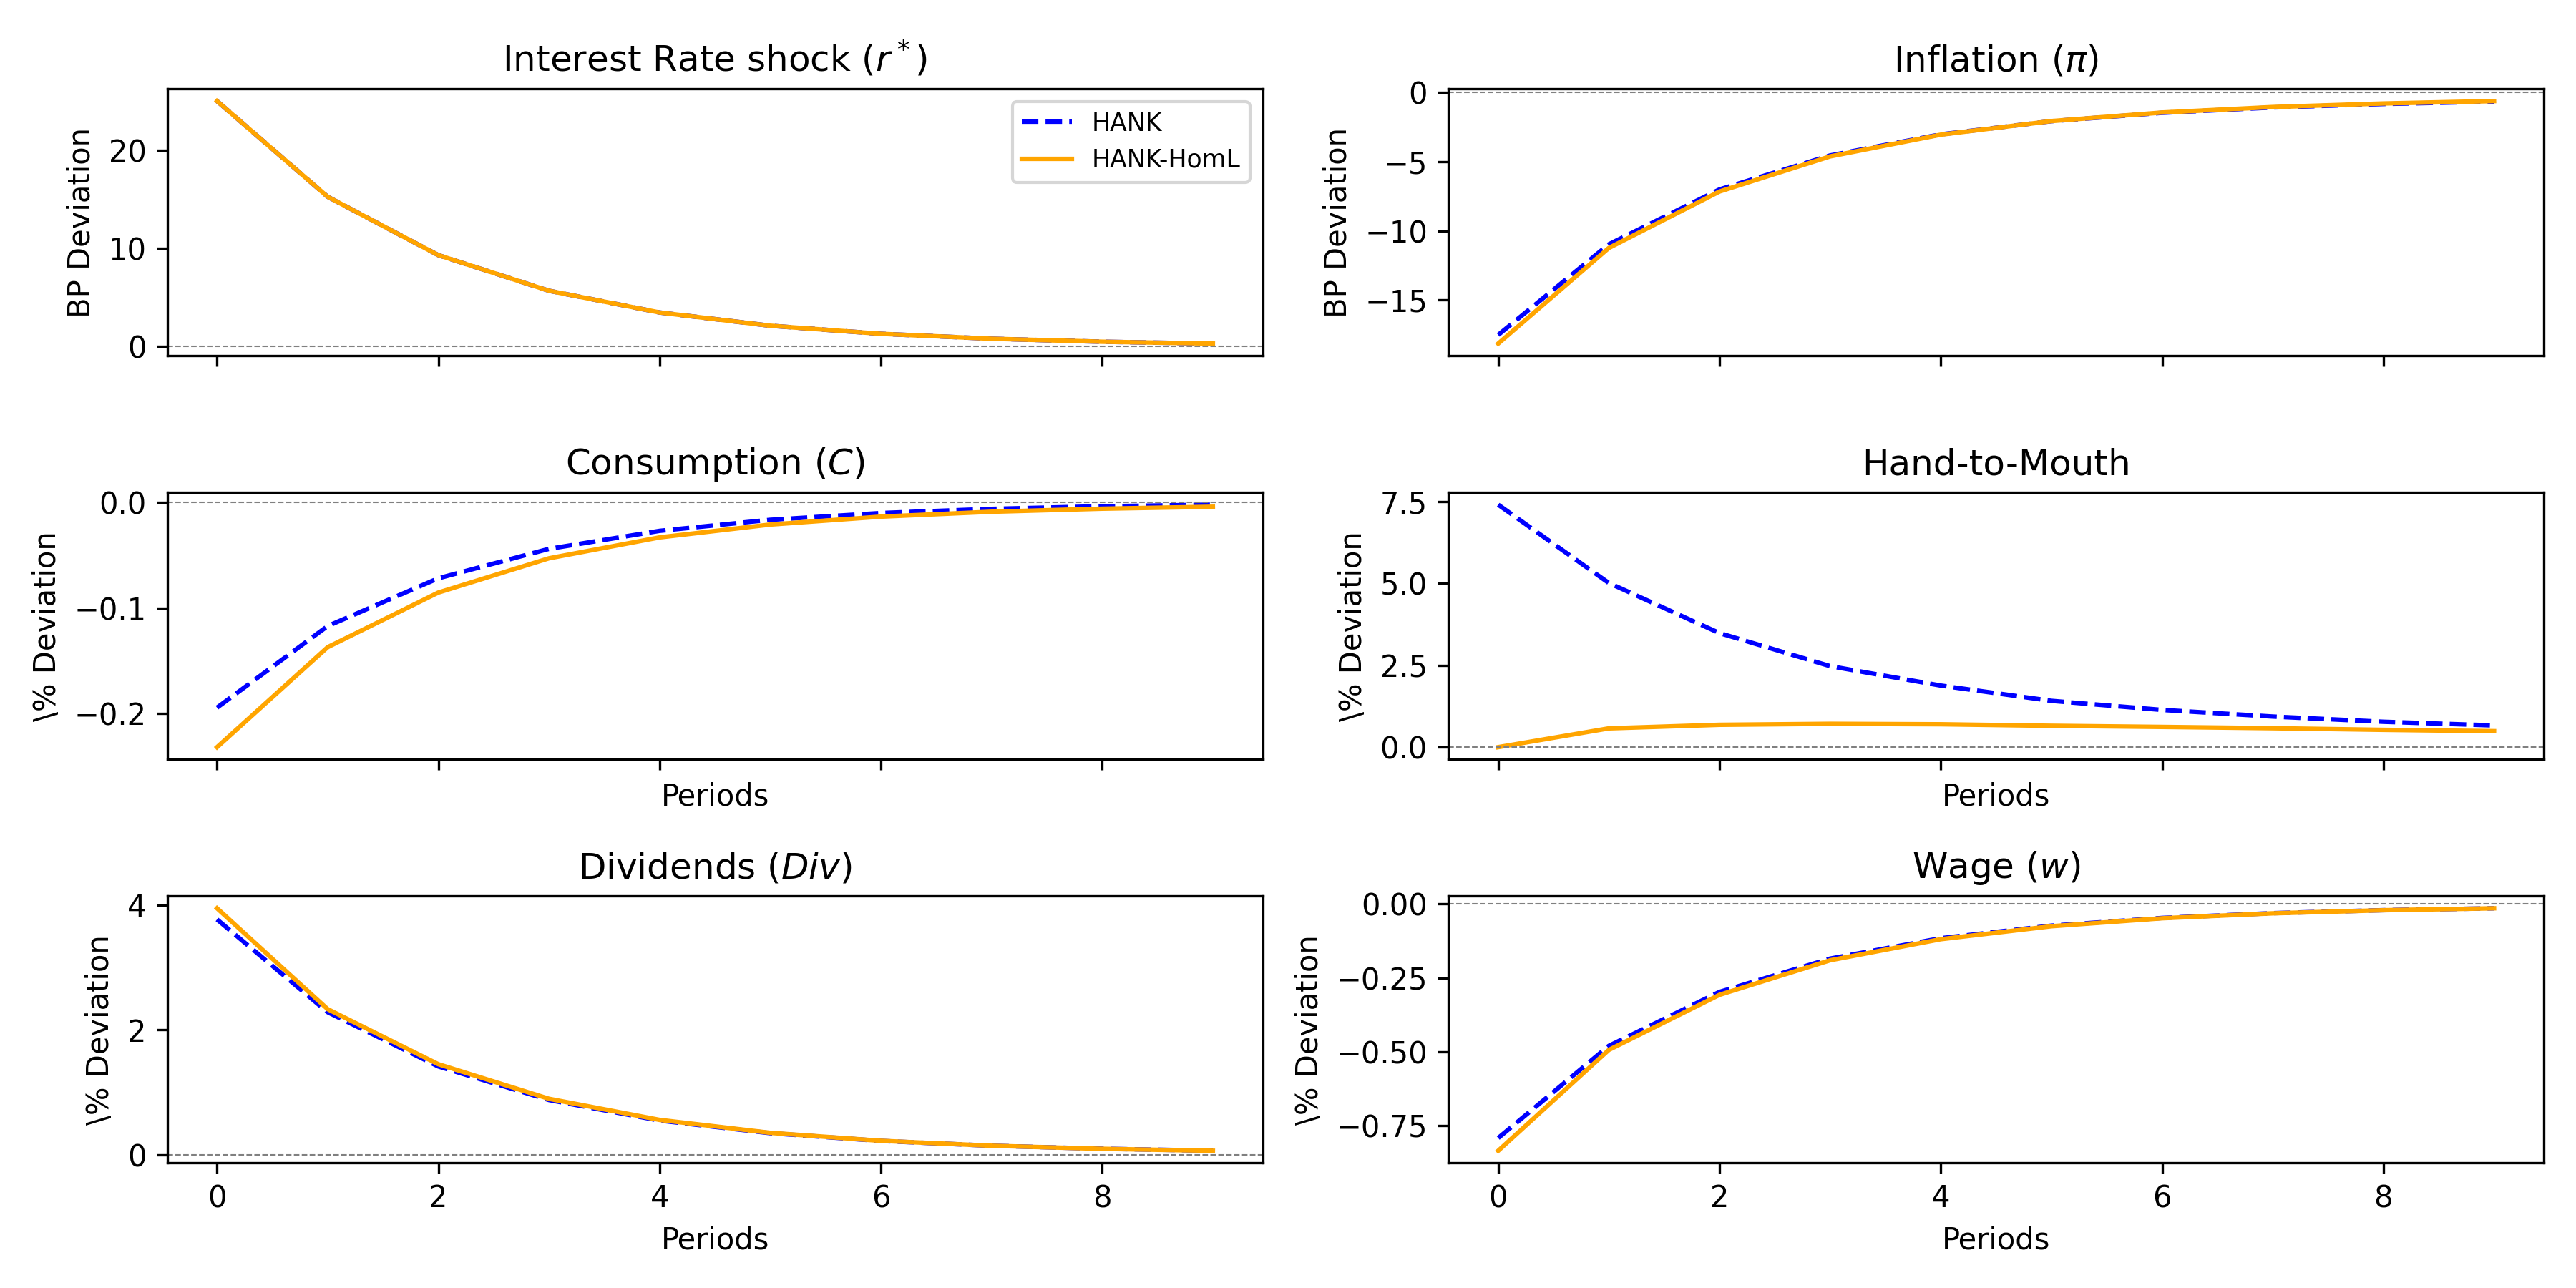
\includegraphics[width=0.95\textwidth]{figures_final/HANK_irfs_core_vars.png}
  \label{fig:core_irfs}
\end{figure}


\begin{figure}[h!]
  \centering
  \caption{Labor Supply Responses Across the Income Distribution}
  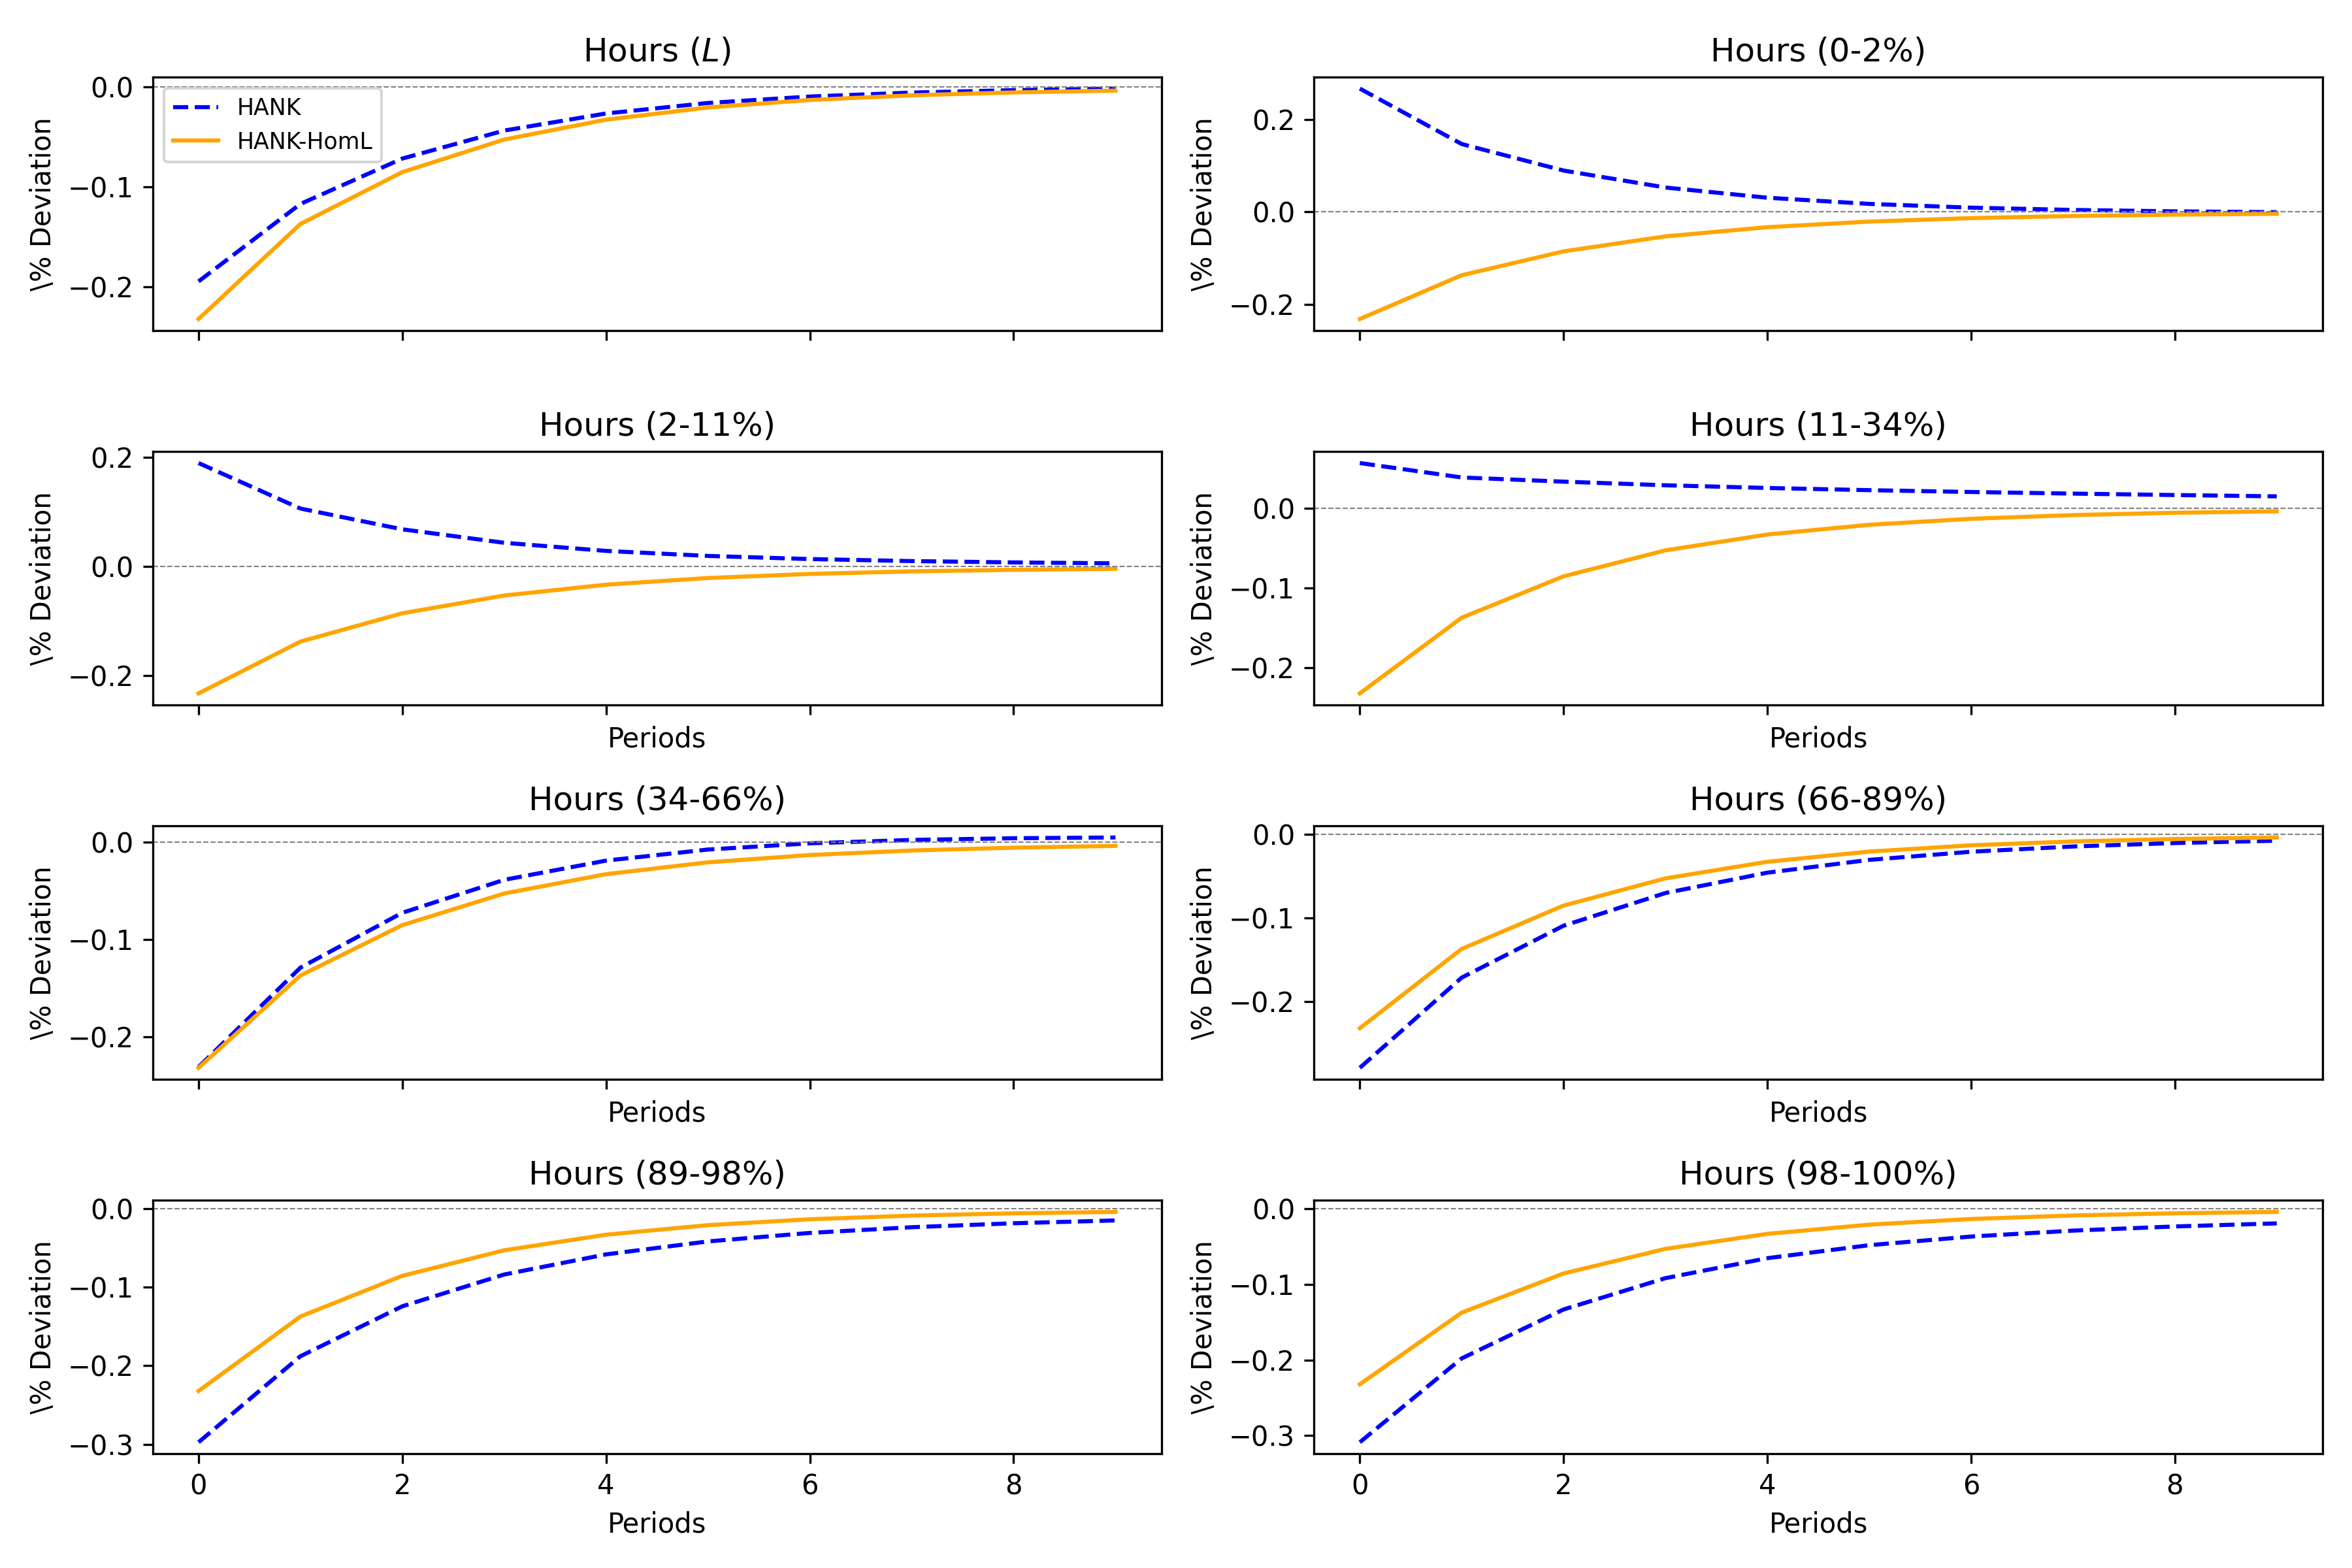
\includegraphics[width=0.95\textwidth]{figures_final/HANK_irfs_H_bins.png}
  \label{fig:L_bins_irfs}
\end{figure}

\begin{figure}[h!]
  \centering
  \caption{Consumption Responses Across the Income Distribution}
  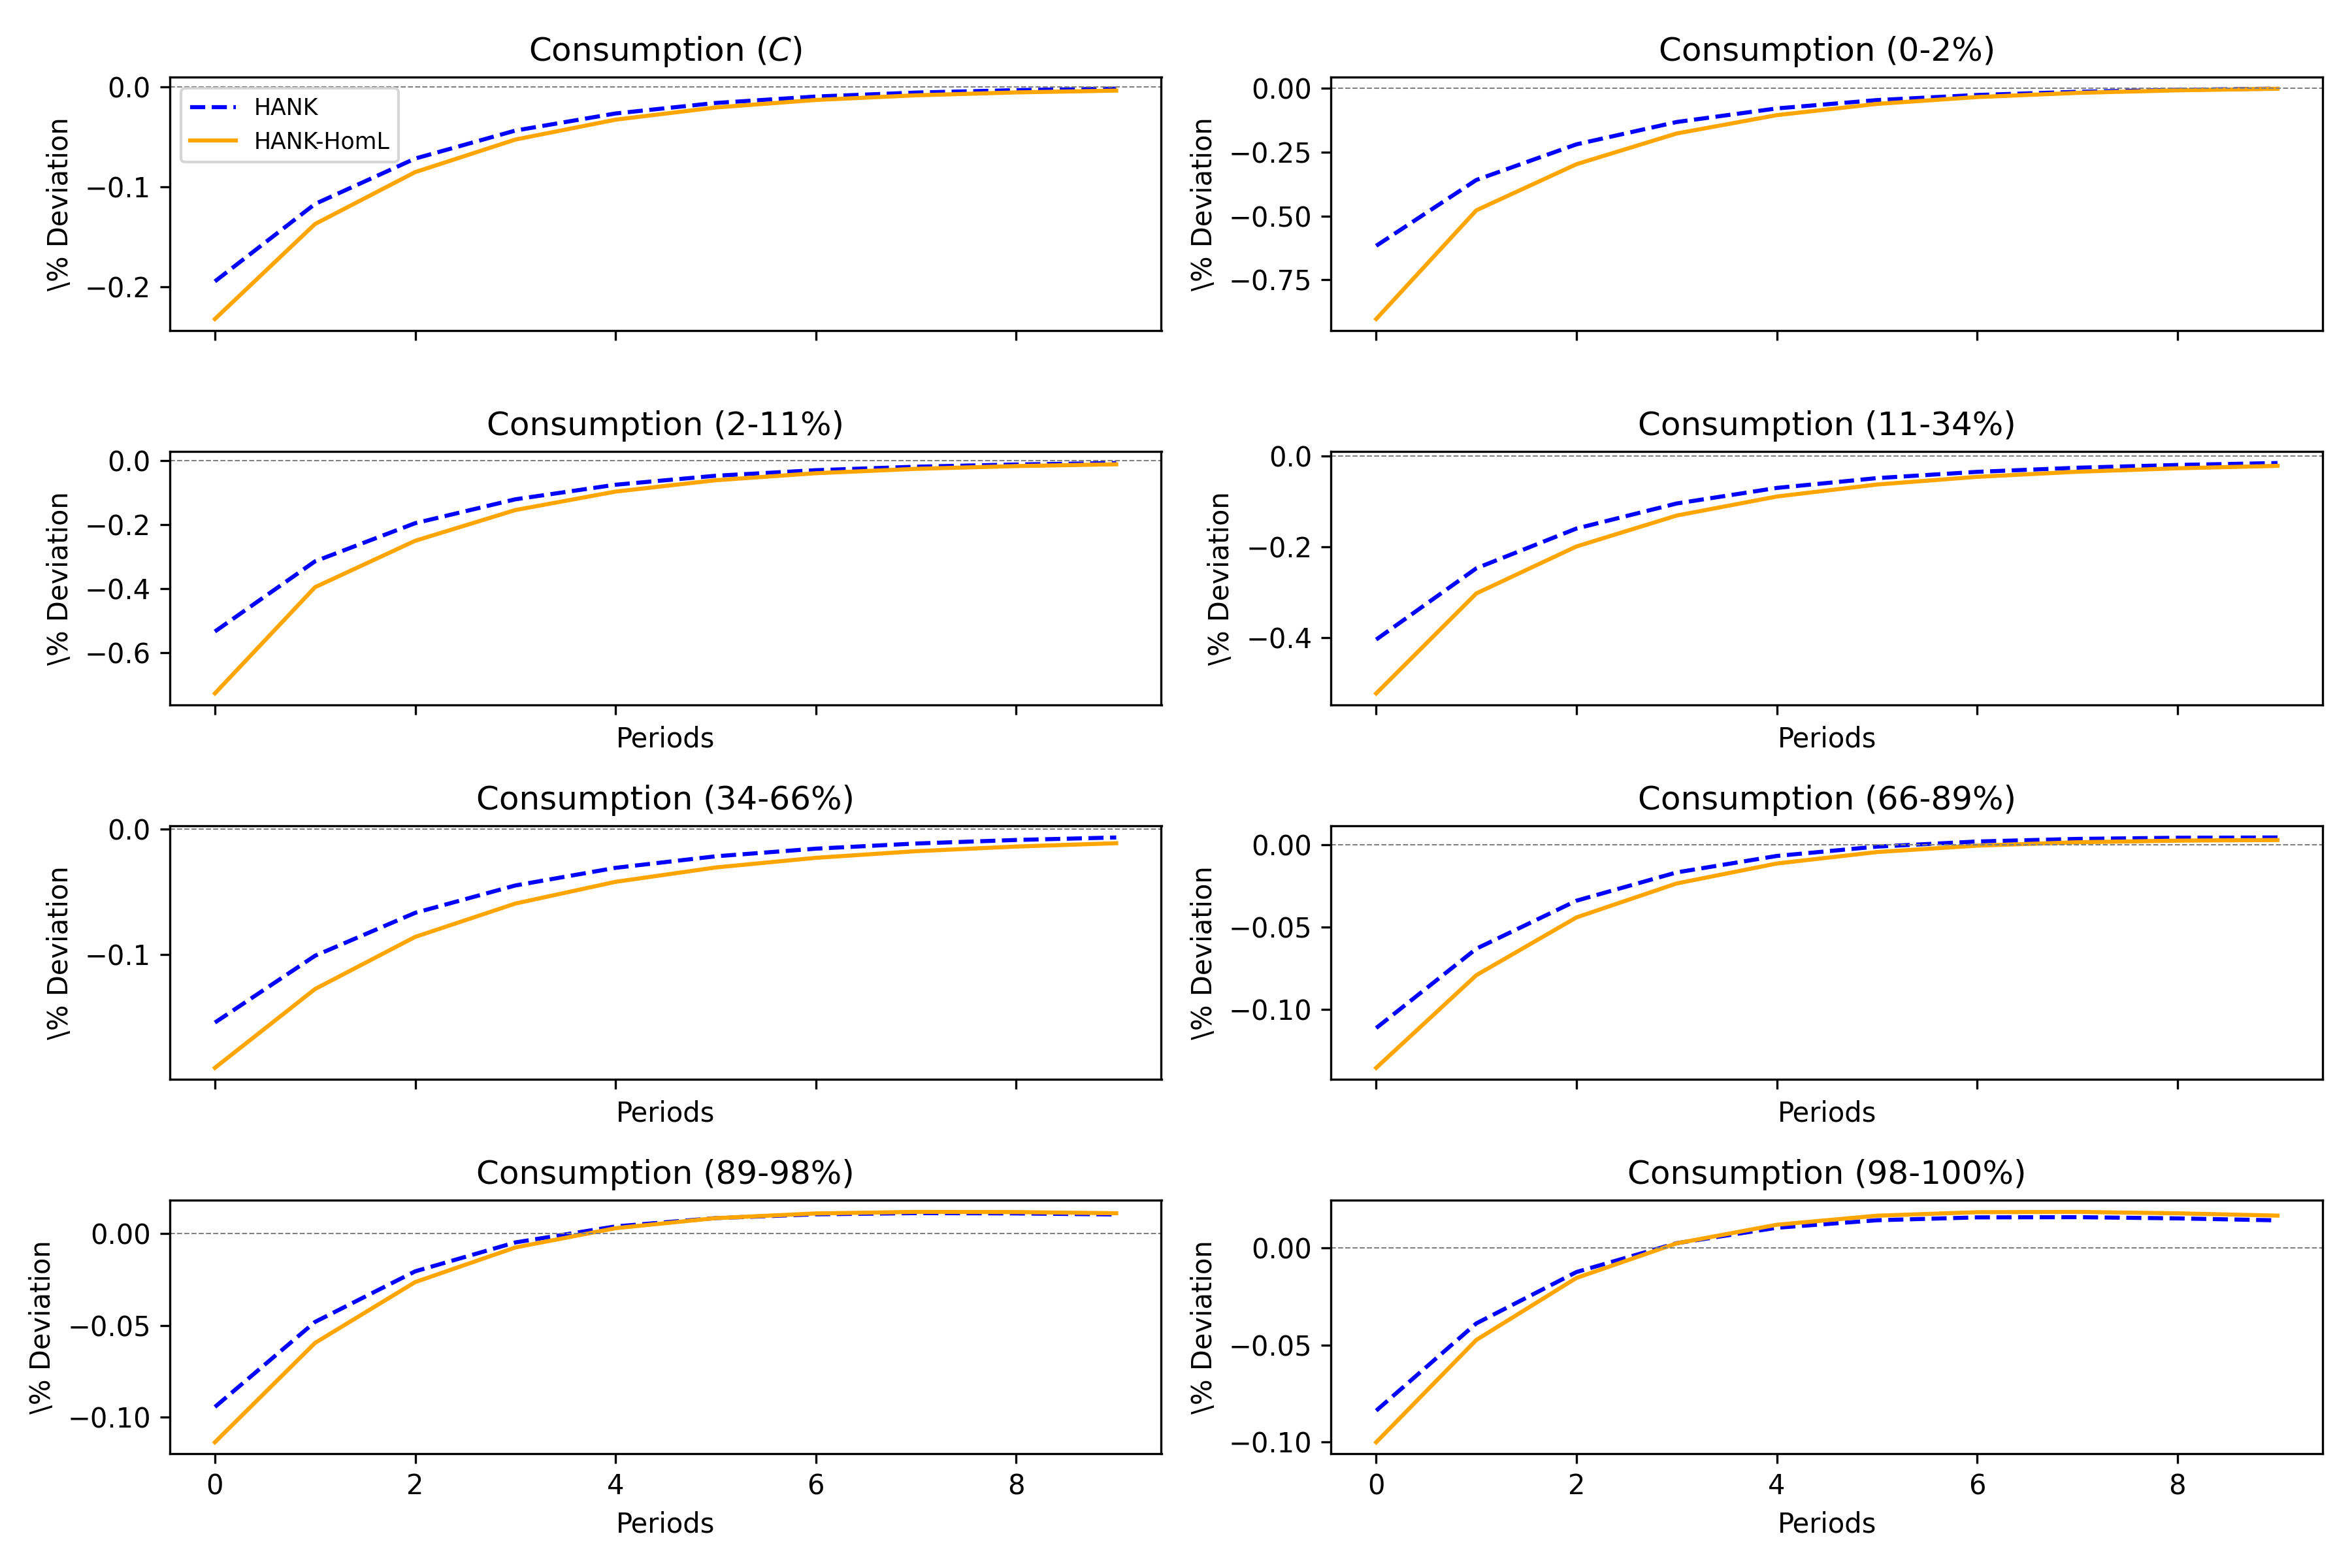
\includegraphics[width=0.95\textwidth]{figures_final/HANK_irfs_C_bins.png}
  \label{fig:C_bins_irfs}
\end{figure}

\begin{figure}[h!]
  \centering
  \caption{Contribution of each income bin to the aggregate response (absolute deviations in basis points). Stacked bars show bin-level components, and the dashed line in each panel reports the aggregate response (sum across bins).}
  \begin{subfigure}[b]{0.45\textwidth}
    \centering
    \caption{Hours}
    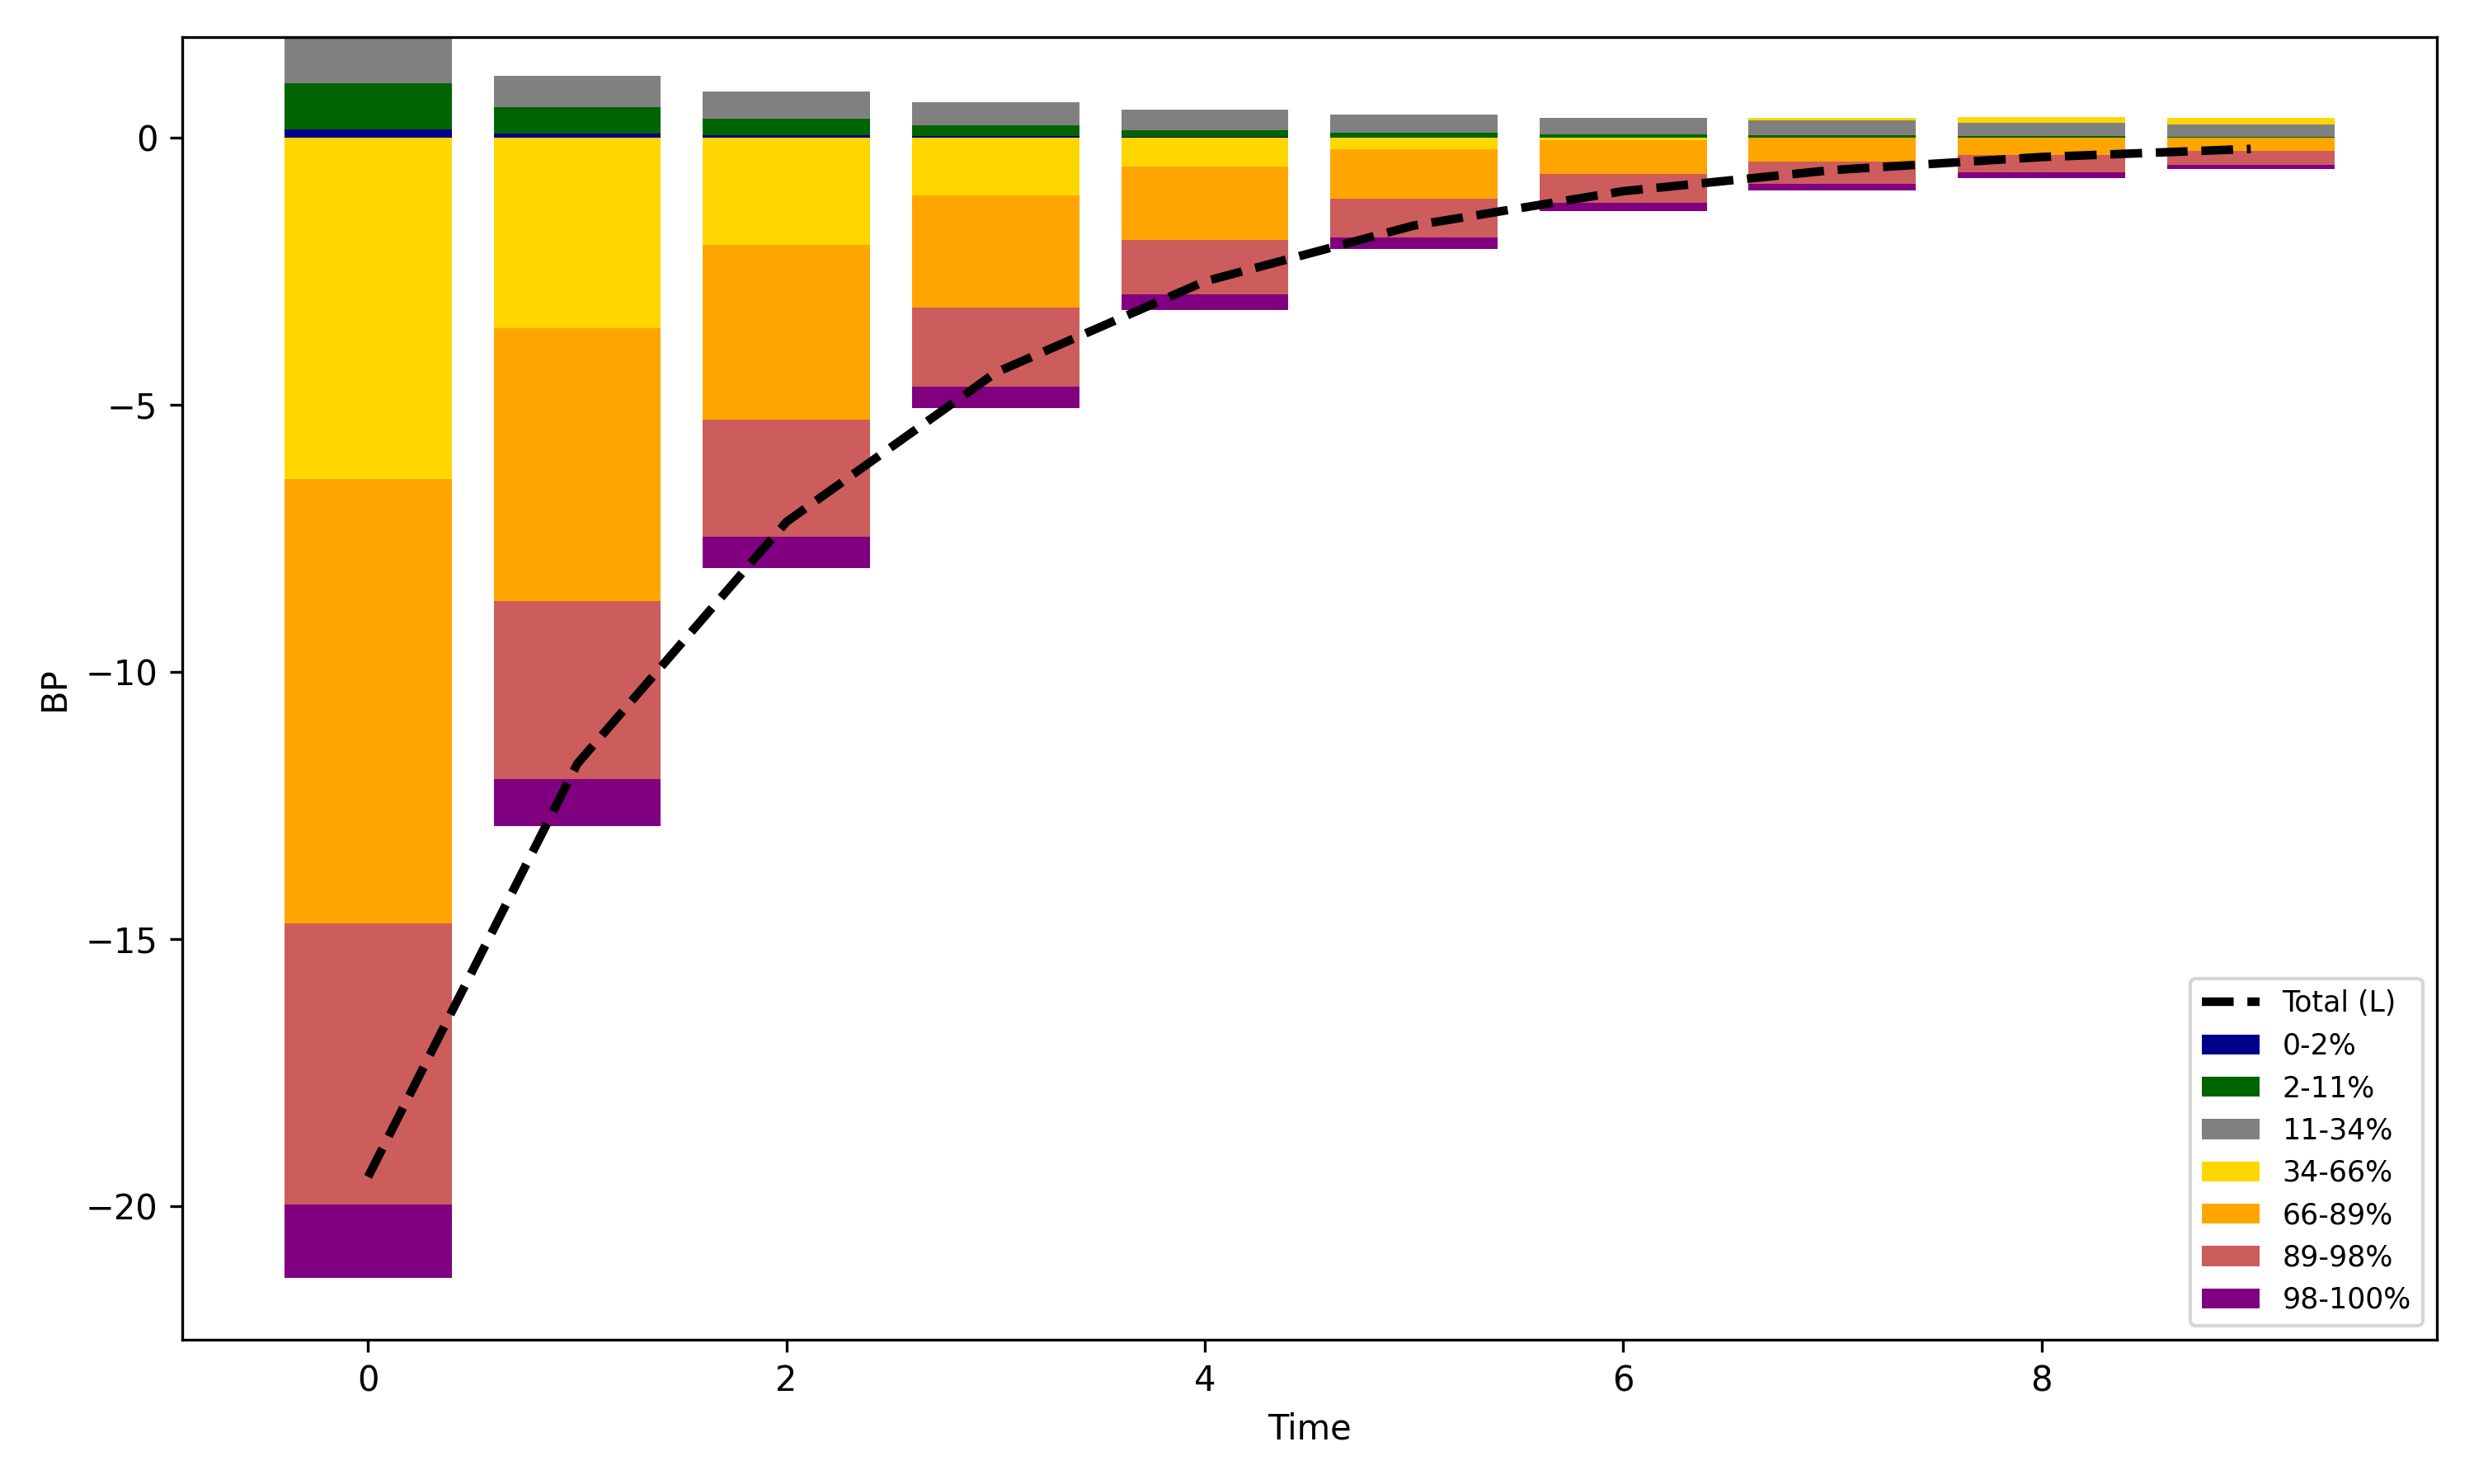
\includegraphics[width=\textwidth]{figures_final/HANK_HetL_bins_L_contribution.png}
  \end{subfigure}%
  \hfill
  \begin{subfigure}[b]{0.45\textwidth}
    \centering
    
  %\caption{Contribution of each income bin to the aggregate response.}
    \caption{Consumption}
    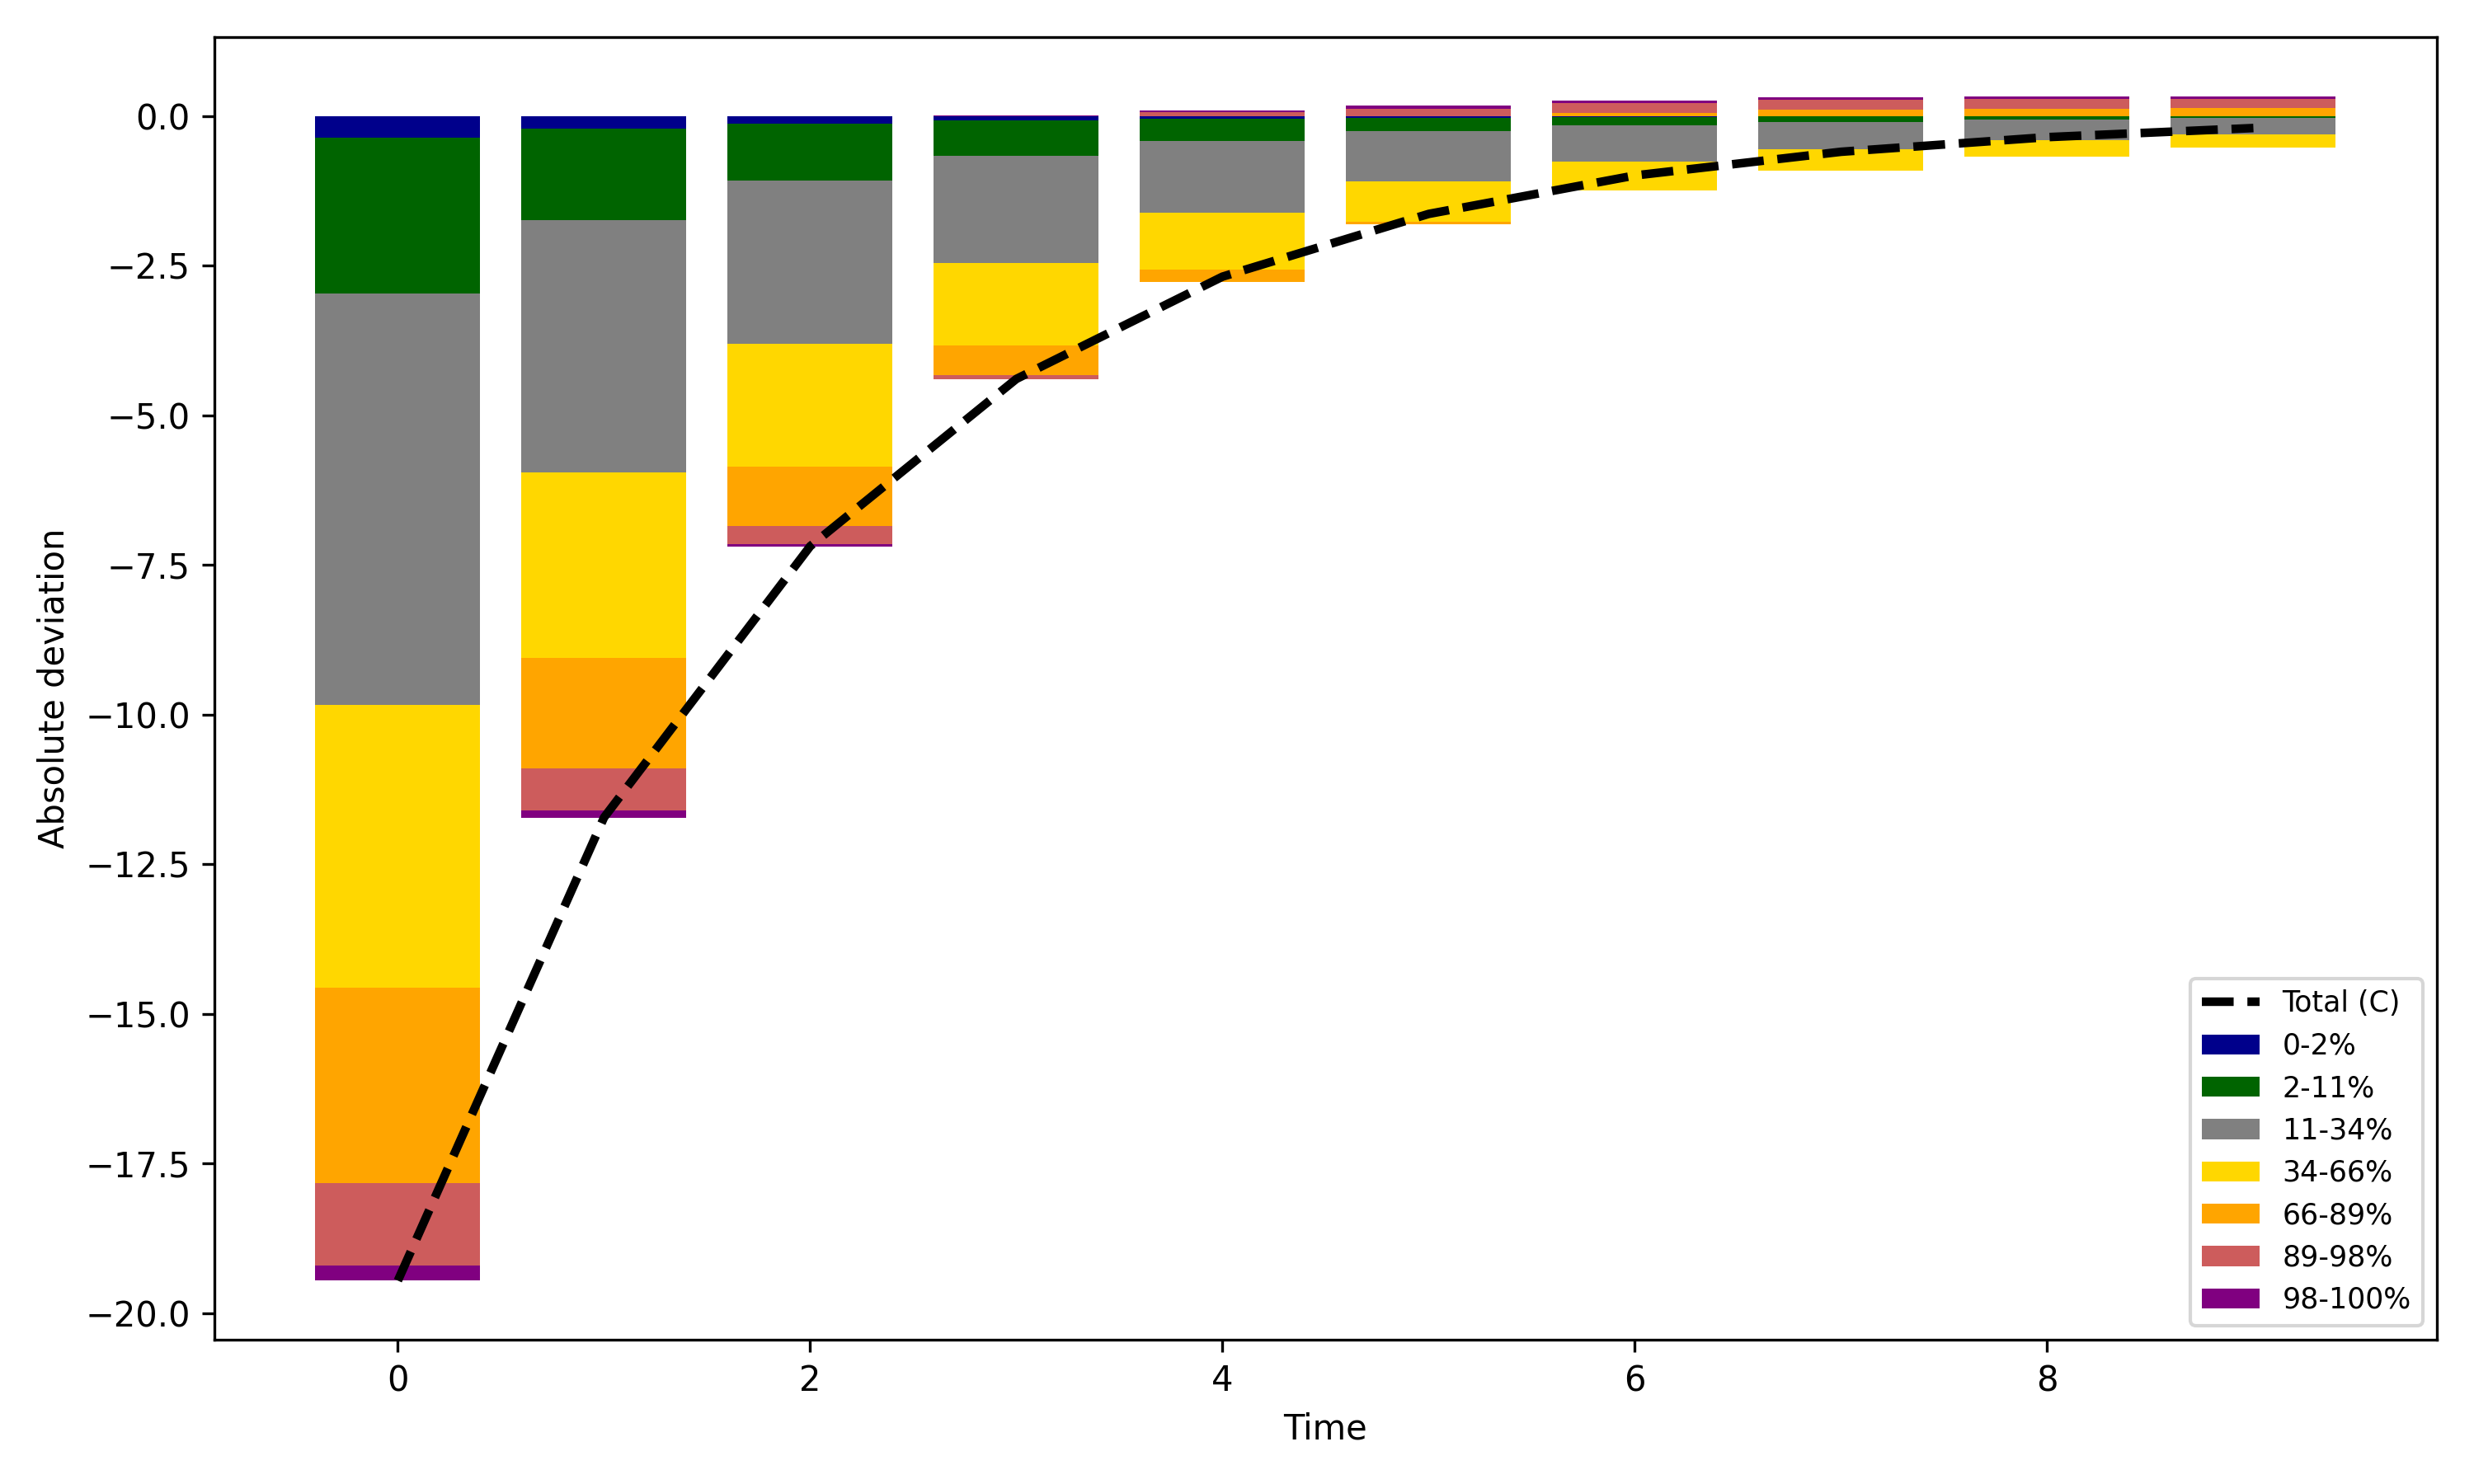
\includegraphics[width=\textwidth]{figures_final/HANK_HetL_bins_C_contribution.png}
  \end{subfigure}
  \label{fig:contribution}
\end{figure}

% \begin{figure}[h!]
%   \centering
%     \centering
%     \includegraphics[width=\textwidth]{figures_final/HANK_HetL_bins_L_contribution_EIS025.png}
%   \caption{Contribution of each income bin to the aggregate response.}
%   \label{fig:contribution_alt}
% \end{figure}



\clearpage
\bibliographystyle{kluwer}
\bibliography{biblio_}
\end{document}
